\title{平面向量与解三角形（2016--2025 高考真题）}
\author{}
\date{}
\maketitle
\noindent 本专题共 138 道题，按年份排列。每题标注原卷与原题号。

\section*{2016 年}

\begin{question}[points=5]
\textbf{来源：}2016 年 全国III卷-理科，第 3 题\par
已知向量 $\overrightarrow{BA}=(\frac{1}{2},\frac{\sqrt{3}}{2})$, $\overrightarrow{BC}=(\frac{\sqrt{3}}{2},\frac{1}{2})$, 则 $\angle ABC=$
\begin{choices}
  \item $30^\circ$
  \item $45^\circ$
  \item $60^\circ$
  \item $120^\circ$
\end{choices}
\begin{solution}
\textbf{答案：}$30^\circ$

\textbf{分析：}根据向量 $\overrightarrow{BA},\overrightarrow{BC}$ 的坐标求出 $\overrightarrow{BA}\cdot\overrightarrow{BC},|\overrightarrow{BA}|,|\overrightarrow{BC}|$ 的值, 从而根据向量夹角余弦公式求出 $\cos\angle ABC$, 根据范围得出 $\angle ABC$.

\textbf{详解：}$\overrightarrow{BA}=(\frac{1}{2},\frac{\sqrt{3}}{2}),\overrightarrow{BC}=(\frac{\sqrt{3}}{2},\frac{1}{2})$, $|\overrightarrow{BA}|=1,|\overrightarrow{BC}|=1,\overrightarrow{BA}\cdot\overrightarrow{BC}=\frac{\sqrt{3}}{2}$, $\therefore \cos\angle ABC=\frac{\overrightarrow{BA}\cdot\overrightarrow{BC}}{|\overrightarrow{BA}||\overrightarrow{BC}|}=\frac{\sqrt{3}}{2}$, 又 $0^\circ\le\angle ABC\le180^\circ$, $\therefore\angle ABC=30^\circ$, 故选 A.
\end{solution}
\end{question}

\begin{question}[points=5]
\textbf{来源：}2016 年 全国III卷-理科，第 8 题\par
在 $\triangle ABC$ 中, $B=\frac{\pi}{4}$, $BC$ 边上的高等于 $\frac{1}{3}BC$, 则 $\cos A$ 等于
\begin{choices}
  \item $\frac{3\sqrt{10}}{10}$
  \item $\frac{\sqrt{10}}{10}$
  \item $-\frac{\sqrt{10}}{10}$
  \item $-\frac{3\sqrt{10}}{10}$
\end{choices}
\begin{solution}
\textbf{答案：}$-\frac{\sqrt{10}}{10}$

\textbf{分析：}作出图形, 令 $\angle DAC=\theta$, 利用两角和的余弦求 $\cos A$.

\textbf{详解：}设 $\triangle ABC$ 中角 $A,B,C$ 对应的边分别为 $a,b,c$, $AD\perp BC$ 于 $D$, 令 $\angle DAC=\theta$. $\because B=\frac{\pi}{4}, BC$ 边上的高 $AD=h=\frac{1}{3}BC=\frac{a}{3}$, $\therefore BD=AD=\frac{a}{3}, CD=\frac{2a}{3}$. 在 $\mathrm{Rt}\triangle ADC$ 中, $\cos\theta=\frac{AD}{AC}=\frac{\frac{a}{3}}{\sqrt{(\frac{a}{3})^2+(\frac{2a}{3})^2}}=\frac{\sqrt{5}}{5}$, 故 $\sin\theta=\frac{2\sqrt{5}}{5}$, $\therefore \cos A=\cos(\frac{\pi}{4}+\theta)=\cos\frac{\pi}{4}\cos\theta-\sin\frac{\pi}{4}\sin\theta=\frac{\sqrt{2}}{2}\cdot\frac{\sqrt{5}}{5}-\frac{\sqrt{2}}{2}\cdot\frac{2\sqrt{5}}{5}=-\frac{\sqrt{10}}{10}$, 故选 C.
\end{solution}
\end{question}

\begin{question}[points=5]
\textbf{来源：}2016 年 全国III卷-文科，第 3 题\par
已知向量 $\overrightarrow{BA}=(\dfrac{1}{2},\dfrac{\sqrt{3}}{2})$, $\overrightarrow{BC}=(\dfrac{\sqrt{3}}{2},\dfrac{1}{2})$, 则 $\angle ABC=$ ( )
\begin{choices}
  \item $30^{\circ}$
  \item $45^{\circ}$
  \item $60^{\circ}$
  \item $120^{\circ}$
\end{choices}
\begin{solution}
\textbf{答案：}$30^{\circ}$

\textbf{分析：}根据向量 $\overrightarrow{BA}$ 和 $\overrightarrow{BC}$ 的坐标求出 $\overrightarrow{BA}\cdot\overrightarrow{BC}$ 及 $|\overrightarrow{BA}|,|\overrightarrow{BC}|$ 的值, 从而根据向量夹角余弦公式即可求出 $\cos\angle ABC$ 的值, 根据 $\angle ABC$ 的范围便可得出 $\angle ABC$ 的值.

\textbf{详解：}$\overrightarrow{BA}=(\dfrac{1}{2},\dfrac{\sqrt{3}}{2})$, $\overrightarrow{BC}=(\dfrac{\sqrt{3}}{2},\dfrac{1}{2})$; 则 $\overrightarrow{BA}\cdot\overrightarrow{BC}=\dfrac{1}{2}\cdot\dfrac{\sqrt{3}}{2}+\dfrac{\sqrt{3}}{2}\cdot\dfrac{1}{2}=\dfrac{\sqrt{3}}{2}$, $|\overrightarrow{BA}|=1$, $|\overrightarrow{BC}|=1$; 所以 $\cos\angle ABC=\dfrac{\overrightarrow{BA}\cdot\overrightarrow{BC}}{|\overrightarrow{BA}||\overrightarrow{BC}|}=\dfrac{\sqrt{3}}{2}$; 又 $0^{\circ}\le\angle ABC\le180^{\circ}$; 所以 $\angle ABC=30^{\circ}$. 故选 A.
\end{solution}
\end{question}

\begin{question}[points=5]
\textbf{来源：}2016 年 全国III卷-文科，第 9 题\par
在 $\triangle ABC$ 中, $B=\dfrac{\pi}{4}$, $BC$ 边上的高等于 $\dfrac{1}{3}BC$, 则 $\sin A=$ ( )
\begin{choices}
  \item $\dfrac{3}{10}$
  \item $\dfrac{\sqrt{10}}{10}$
  \item $\dfrac{\sqrt{5}}{5}$
  \item $\dfrac{3\sqrt{10}}{10}$
\end{choices}
\begin{solution}
\textbf{答案：}$\dfrac{3\sqrt{10}}{10}$

\textbf{分析：}由已知, 结合勾股定理和余弦定理, 求出 $AB$, $AC$, 再由三角形面积公式, 可得 $\sin A$.

\textbf{详解：}在 $\triangle ABC$ 中, $B=\dfrac{\pi}{4}$, $BC$ 边上的高等于 $\dfrac{1}{3}BC$, 所以 $AB=\dfrac{\sqrt{2}}{3}BC$. 由余弦定理 $AC^2=AB^2+BC^2-2\cdot AB\cdot BC\cdot\cos B=\dfrac{2}{9}BC^2+BC^2-2\cdot\dfrac{\sqrt{2}}{3}BC\cdot BC\cdot\dfrac{\sqrt{2}}{2}=\dfrac{2}{9}BC^2+BC^2-\dfrac{2}{3}BC^2=\dfrac{5}{9}BC^2$, 故 $AC=\dfrac{\sqrt{5}}{3}BC$. 由面积公式 $\dfrac{1}{2}\cdot BC\cdot\dfrac{1}{3}BC=\dfrac{1}{2}\cdot AB\cdot AC\cdot\sin A$, 即 $\dfrac{1}{6}BC^2=\dfrac{1}{2}\cdot\dfrac{\sqrt{2}}{3}BC\cdot\dfrac{\sqrt{5}}{3}BC\cdot\sin A$, 解得 $\sin A=\dfrac{3\sqrt{10}}{10}$. 故选 D.
\end{solution}
\end{question}

\begin{question}[points=5]
\textbf{来源：}2016 年 全国II卷-理科，第 3 题\par
已知向量$\overrightarrow{a}=(1,m)$，$\overrightarrow{b}=(3,-2)$，且$(\overrightarrow{a}+\overrightarrow{b})\perp\overrightarrow{b}$，则$m=$（\quad）
\begin{choices}
  \item $-8$
  \item $-6$
  \item $6$
  \item $8$
\end{choices}
\begin{solution}
\textbf{答案：}$8$

\textbf{分析：}求出向量$\overrightarrow{a}+\overrightarrow{b}$的坐标，根据向量垂直的充要条件，构造关于$m$的方程，解得答案．

\textbf{详解：}$\overrightarrow{a}+\overrightarrow{b}=(4,m-2)$，由$(\overrightarrow{a}+\overrightarrow{b})\perp\overrightarrow{b}$得$4\times3+(m-2)\times(-2)=0$，解得$m=8$．故选D．
\end{solution}
\end{question}

\begin{question}[points=5]
\textbf{来源：}2016 年 全国II卷-理科，第 13 题\par
$\triangle ABC$的内角$A$，$B$，$C$的对边分别为$a$，$b$，$c$，若$\cos A=\frac{4}{5}$，$\cos C=\frac{5}{13}$，$a=1$，则$b=$．
\fillin[{$\frac{21}{13}$}]
\begin{solution}
\textbf{答案：}$\frac{21}{13}$

\textbf{分析：}运用同角的平方关系可得$\sin A$，$\sin C$，再由诱导公式和两角和的正弦公式，可得$\sin B$，运用正弦定理可得$b=\frac{a\sin B}{\sin A}$，代入计算即可得到所求值．

\textbf{详解：}$\sin A=\frac{3}{5}$，$\sin C=\frac{12}{13}$，$\sin B=\sin(A+C)=\frac{3}{5}\times\frac{5}{13}+\frac{4}{5}\times\frac{12}{13}=\frac{63}{65}$，由正弦定理$b=\frac{a\sin B}{\sin A}=\frac{1\times\frac{63}{65}}{\frac{3}{5}}=\frac{21}{13}$．
\end{solution}
\end{question}

\begin{question}[points=5]
\textbf{来源：}2016 年 全国II卷-文科，第 13 题\par
已知向量$\vec{a}=(m,4)$，$\vec{b}=(3,-2)$，且$\vec{a}\parallel\vec{b}$，则$m=$
\fillin[{$-6$}]
\begin{solution}
\textbf{答案：}$-6$

\textbf{分析：}由向量共线得$m\times(-2)=4\times3$，解得$m=-6$。
\end{solution}
\end{question}

\begin{question}[points=5]
\textbf{来源：}2016 年 全国II卷-文科，第 15 题\par
$\triangle ABC$的内角$A$，$B$，$C$的对边分别为$a$，$b$，$c$，若$\cos A=\frac{4}{5}$，$\cos C=\frac{5}{13}$，$a=1$，则$b=$
\fillin[{$\frac{21}{13}$}]
\begin{solution}
\textbf{答案：}$\frac{21}{13}$

\textbf{分析：}$\sin A=\frac{3}{5}$，$\sin C=\frac{12}{13}$，$\sin B=\sin(A+C)=\frac{63}{65}$，由正弦定理$b=\frac{a\sin B}{\sin A}=\frac{1\times\frac{63}{65}}{\frac{3}{5}}=\frac{21}{13}$。
\end{solution}
\end{question}

\begin{question}[points=5]
\textbf{来源：}2016 年 全国I卷-理科，第 13 题\par
设向量$\vec{a}=(m,1)$，$\vec{b}=(1,2)$，且$|\vec{a}+\vec{b}|^2=|\vec{a}|^2+|\vec{b}|^2$，则$m=$．
\fillin[{$-2$}]
\begin{solution}
\textbf{答案：}$-2$

\textbf{分析：}利用已知条件，通过数量积判断两个向量垂直，然后列出方程求解即可．

\textbf{详解：}解：$|\vec{a}+\vec{b}|^2=|\vec{a}|^2+|\vec{b}|^2$，可得$\vec{a}\cdot\vec{b}=0$．向量$\vec{a}=(m,1)$，$\vec{b}=(1,2)$，可得$m+2=0$，解得$m=-2$．故答案为：$-2$．
\end{solution}
\end{question}

\begin{question}[points=12]
\textbf{来源：}2016 年 全国I卷-理科，第 17 题\par
$\triangle ABC$的内角$A$，$B$，$C$的对边分别为$a$，$b$，$c$，已知$2\cos C(a\cos B+b\cos A)=c$．

（Ⅰ）求$C$；

（Ⅱ）若$c=\sqrt{7}$，$\triangle ABC$的面积为$\frac{3\sqrt{3}}{2}$，求$\triangle ABC$的周长．
\begin{solution}
\textbf{答案：}（Ⅰ）$C=\frac{\pi}{3}$；（Ⅱ）$5+\sqrt{7}$

\textbf{分析：}（Ⅰ）已知等式利用正弦定理化简，整理后利用两角和与差的正弦函数公式及诱导公式化简，根据$\sin C$不为$0$求出$\cos C$的值，即可确定出出$C$的度数；（2）利用余弦定理列出关系式，利用三角形面积公式列出关系式，求出$a+b$的值，即可求$\triangle ABC$的周长．

\textbf{详解：}解：（Ⅰ）因为在$\triangle ABC$中，$0<C<\pi$，所以$\sin C\neq0$已知等式利用正弦定理化简得：$2\cos C(\sin A\cos B+\sin B\cos A)=\sin C$，整理得：$2\cos C\sin(A+B)=\sin C$，即$2\cos C\sin(\pi-(A+B))=\sin C$，$2\cos C\sin C=\sin C$，所以$\cos C=\frac{1}{2}$，所以$C=\frac{\pi}{3}$；（Ⅱ）由余弦定理得$7=a^2+b^2-2ab\cdot\frac{1}{2}$，所以$(a+b)^2-3ab=7$，因为$S=\frac{1}{2}ab\sin C=\frac{\sqrt{3}}{4}ab=\frac{3\sqrt{3}}{2}$，所以$ab=6$，所以$(a+b)^2-18=7$，所以$a+b=5$，所以$\triangle ABC$的周长为$5+\sqrt{7}$．
\end{solution}
\end{question}

\begin{question}[points=5]
\textbf{来源：}2016 年 全国I卷-文科，第 4 题\par
$\triangle ABC$的内角$A$、$B$、$C$的对边分别为$a$、$b$、$c$。已知$a=\sqrt{5}$，$c=2$，$\cos A=\frac{2}{3}$，则$b=$
\begin{choices}
  \item $\sqrt{2}$
  \item $\sqrt{3}$
  \item $2$
  \item $3$
\end{choices}
\begin{solution}
\textbf{答案：}$3$

\textbf{分析：}由余弦定理可得$\cos A=\frac{b^2+c^2-a^2}{2bc}$，利用已知整理可得$3b^2-8b-3=0$，从而解得$b$的值。

\textbf{详解：}$\because a=\sqrt{5}$，$c=2$，$\cos A=\frac{2}{3}$，$\therefore$由余弦定理可得：$\cos A=\frac{b^2+c^2-a^2}{2bc}=\frac{b^2+4-5}{4b}=\frac{b^2-1}{4b}=\frac{2}{3}$，整理可得：$3b^2-8b-3=0$，$\therefore$解得：$b=3$或$-\frac{1}{3}$（舍去）。故选：$D$。
\end{solution}
\end{question}

\begin{question}[points=5]
\textbf{来源：}2016 年 全国I卷-文科，第 13 题\par
设向量$\vec{a}=(x,x+1)$，$\vec{b}=(1,2)$，且$\vec{a}\perp\vec{b}$，则$x=$
\fillin[{$-\frac{2}{3}$}]
\begin{solution}
\textbf{答案：}$-\frac{2}{3}$

\textbf{分析：}根据向量垂直的充要条件便可得出$\vec{a}\cdot\vec{b}=0$，进行向量数量积的坐标运算即可得出关于$x$的方程，解方程便可得出$x$的值。

\textbf{详解：}$\because \vec{a}\perp\vec{b}$；$\therefore \vec{a}\cdot\vec{b}=0$；即$x+2(x+1)=0$；$\therefore x=-\frac{2}{3}$。故答案为：$-\frac{2}{3}$。
\end{solution}
\end{question}

\section*{2017 年}

\begin{question}[points=5]
\textbf{来源：}2017 年 全国III卷-理科，第 12 题\par
在矩形$ABCD$中，$AB=1$，$AD=2$，动点$P$在以点$C$为圆心且与$BD$相切的圆上．若$\overrightarrow{AP}=\lambda\overrightarrow{AB}+\mu\overrightarrow{AD}$，则$\lambda+\mu$的最大值为（ ）

\begin{center}
  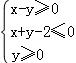
\includegraphics[width=.42\linewidth]{assets/asset-013-01.jpg}
\end{center}
\begin{choices}
  \item $3$
  \item $2\sqrt{2}$
  \item $\sqrt{5}$
  \item $2$
\end{choices}
\begin{solution}
\textbf{答案：}$A$

\textbf{分析：}如图：以$A$为原点，以$AB$，$AD$所在的直线为$x$，$y$轴建立如图所示的坐标系，先求出圆的标准方程，再设点$P$的坐标为$(\frac{2\sqrt{5}}{5}\cos\theta+1，\frac{2\sqrt{5}}{5}\sin\theta+2)$，根据$\overrightarrow{AP}=\lambda\overrightarrow{AB}+\mu\overrightarrow{AD}$，求出$\lambda$，$\mu$，根据三角函数的性质即可求出最值。

\textbf{详解：}如图：以$A$为原点，以$AB$，$AD$所在的直线为$x$，$y$轴建立如图所示的坐标系，则$A(0,0)$，$B(1,0)$，$D(0,2)$，$C(1,2)$。因为动点$P$在以点$C$为圆心且与$BD$相切的圆上，设圆的半径为$r$。因为$BC=2$，$CD=1$，所以$BD=\sqrt{BC^2+CD^2}=\sqrt{5}$。所以$\frac{1}{2}BC\cdot CD=\frac{1}{2}BD\cdot r$，所以$r=\frac{2\sqrt{5}}{5}$。所以圆的方程为$(x-1)^2+(y-2)^2=\frac{4}{5}$。设点$P$的坐标为$(\frac{2\sqrt{5}}{5}\cos\theta+1，\frac{2\sqrt{5}}{5}\sin\theta+2)$。因为$\overrightarrow{AP}=\lambda\overrightarrow{AB}+\mu\overrightarrow{AD}$，所以$(\frac{2\sqrt{5}}{5}\cos\theta+1，\frac{2\sqrt{5}}{5}\sin\theta+2)=\lambda(1,0)+\mu(0,2)=(\lambda,2\mu)$。所以$\frac{2\sqrt{5}}{5}\cos\theta+1=\lambda$，$\frac{2\sqrt{5}}{5}\sin\theta+2=2\mu$。所以$\lambda+\mu=\frac{\sqrt{5}}{5}\cos\theta+\frac{\sqrt{5}}{5}\sin\theta+2=\sin(\theta+\varphi)+2$，其中$\tan\varphi=2$。因为$-1\le\sin(\theta+\varphi)\le1$，所以$1\le\lambda+\mu\le3$，故$\lambda+\mu$的最大值为$3$。故选A。
\end{solution}
\end{question}

\begin{question}[points=12]
\textbf{来源：}2017 年 全国III卷-理科，第 17 题\par
$\triangle ABC$的内角$A$，$B$，$C$的对边分别为$a$，$b$，$c$，已知$\sin A+\sqrt{3}\cos A=0$，$a=2\sqrt{7}$，$b=2$．

（1）求$c$；

（2）设$D$为$BC$边上一点，且$AD\perp AC$，求$\triangle ABD$的面积．
\begin{solution}
\textbf{答案：}（1）$c=4$；（2）$\sqrt{3}$

\textbf{分析：}（1）先根据同角的三角函数的关系求出$A$，再根据余弦定理即可求出；（2）先根据夹角求出$\cos C$，求出$CD$的长，得到$S_{\triangle ABD}=\frac{1}{2}S_{\triangle ABC}$。

\textbf{详解：}解：（1）因为$\sin A+\sqrt{3}\cos A=0$，所以$\tan A=-\sqrt{3}$，因为$0<A<\pi$，所以$A=\frac{2\pi}{3}$。由余弦定理可得$a^2=b^2+c^2-2bc\cos A$，即$28=4+c^2-2\times2c\times(-\frac{1}{2})$，即$c^2+2c-24=0$，解得$c=-6$（舍去）或$c=4$，故$c=4$。
（2）因为$c^2=b^2+a^2-2ab\cos C$，所以$16=28+4-2\times2\sqrt{7}\times2\times\cos C$，所以$\cos C=\frac{2\sqrt{7}}{7}$，所以$CD=\frac{AC}{\cos C}=\frac{2}{\frac{2\sqrt{7}}{7}}=\sqrt{7}$。所以$CD=\frac{1}{2}BC$。因为$S_{\triangle ABC}=\frac{1}{2}AB\cdot AC\cdot\sin\angle BAC=\frac{1}{2}\times4\times2\times\frac{\sqrt{3}}{2}=2\sqrt{3}$，所以$S_{\triangle ABD}=\frac{1}{2}S_{\triangle ABC}=\sqrt{3}$。
\end{solution}
\end{question}

\begin{question}[points=5]
\textbf{来源：}2017 年 全国III卷-文科，第 13 题\par
已知向量$\vec{a}=(-2,3)$，$\vec{b}=(3,m)$，且$\vec{a}\perp\vec{b}$，则$m=$        。
\fillin[{$2$}]
\begin{solution}
\textbf{答案：}$2$

\textbf{分析：}利用平面向量数量积坐标运算法则和向量垂直的性质求解。

\textbf{详解：}$\vec{a}\cdot\vec{b}=(-2)\times3+3m=0$，解得$m=2$。
\end{solution}
\end{question}

\begin{question}[points=5]
\textbf{来源：}2017 年 全国III卷-文科，第 15 题\par
$\triangle ABC$的内角$A,B,C$的对边分别为$a,b,c$，已知$C=60^\circ$，$b=\sqrt{6}$，$c=3$，则$A=$        。
\fillin[{$75^\circ$}]
\begin{solution}
\textbf{答案：}$75^\circ$

\textbf{分析：}根据正弦定理和三角形的内角和计算即可。

\textbf{详解：}由正弦定理$\frac{b}{\sin B}=\frac{c}{\sin C}$，得$\sin B=\frac{b\sin C}{c}=\frac{\sqrt{6}\times\frac{\sqrt{3}}{2}}{3}=\frac{\sqrt{2}}{2}$，因为$b<c$，所以$B=45^\circ$，$A=180^\circ-60^\circ-45^\circ=75^\circ$。
\end{solution}
\end{question}

\begin{question}[points=5]
\textbf{来源：}2017 年 全国II卷-理科，第 12 题\par
已知 $\triangle ABC$ 是边长为 $2$ 的等边三角形，$P$ 为平面 $ABC$ 内一点，则 $\overrightarrow{PA}\cdot(\overrightarrow{PB}+\overrightarrow{PC})$ 的最小值是（   ）
\begin{choices}
  \item $-2$
  \item $-\frac{3}{2}$
  \item $-\frac{4}{3}$
  \item $-1$
\end{choices}
\begin{solution}
\textbf{答案：}$B$

\textbf{分析：}根据条件建立坐标系，求出点的坐标，利用坐标法结合向量数量积的公式进行计算即可。

\textbf{详解：}建立如图所示的坐标系，以 $BC$ 中点为坐标原点，则 $A(0,\sqrt{3})$，$B(-1,0)$，$C(1,0)$，设 $P(x,y)$，则 $\overrightarrow{PA}=(-x,\sqrt{3}-y)$，$\overrightarrow{PB}=(-1-x,-y)$，$\overrightarrow{PC}=(1-x,-y)$，则 $\overrightarrow{PA}\cdot(\overrightarrow{PB}+\overrightarrow{PC})=2x^2-2\sqrt{3}y+2y^2=2[x^2+(y-\frac{\sqrt{3}}{2})^2-\frac{3}{4}]$，$\therefore$ 当 $x=0$，$y=\frac{\sqrt{3}}{2}$ 时，取得最小值 $2\times(-\frac{3}{4})=-\frac{3}{2}$，故选：$B$。
\end{solution}
\end{question}

\begin{question}[points=12]
\textbf{来源：}2017 年 全国II卷-理科，第 17 题\par
$\triangle ABC$ 的内角 $A$，$B$，$C$ 的对边分别为 $a$，$b$，$c$，已知 $\sin(A+C)=8\sin^2\frac{B}{2}$．

（1）求 $\cos B$；

（2）若 $a+c=6$，$\triangle ABC$ 的面积为 $2$，求 $b$．
\begin{solution}
\textbf{答案：}（1）$\cos B=\frac{15}{17}$；（2）$b=2$

\textbf{分析：}（1）利用三角形的内角和定理可知 $A+C=\pi-B$，再利用诱导公式化简 $\sin(A+C)$，利用降幂公式化简 $8\sin^2\frac{B}{2}$，结合 $\sin^2B+\cos^2B=1$，求出 $\cos B$，（2）由（1）可知 $\sin B=\frac{8}{17}$，利用勾面积公式求出 $ac$，再利用余弦定理即可求出 $b$。

\textbf{详解：}（1）$\sin(A+C)=8\sin^2\frac{B}{2}$，$\therefore\sin B=4(1-\cos B)$，$\because\sin^2B+\cos^2B=1$，$\therefore16(1-\cos B)^2+\cos^2B=1$，$\therefore16(1-\cos B)^2+\cos^2B-1=0$，$\therefore16(\cos B-1)^2+(\cos B-1)(\cos B+1)=0$，$\therefore(17\cos B-15)(\cos B-1)=0$，$\therefore\cos B=\frac{15}{17}$；
（2）由（1）可知 $\sin B=\frac{8}{17}$，$\because S_{\triangle ABC}=\frac{1}{2}ac\cdot\sin B=2$，$\therefore ac=\frac{17}{2}$，$\therefore b^2=a^2+c^2-2ac\cos B=a^2+c^2-2\times\frac{17}{2}\times\frac{15}{17}=a^2+c^2-15=(a+c)^2-2ac-15=36-17-15=4$，$\therefore b=2$。
\end{solution}
\end{question}

\begin{question}[points=5]
\textbf{来源：}2017 年 全国II卷-文科，第 4 题\par
设非零向量 $\vec{a}$, $\vec{b}$ 满足 $|\vec{a}+\vec{b}|=|\vec{a}-\vec{b}|$, 则
\begin{choices}
  \item $\vec{a}\perp\vec{b}$
  \item $|\vec{a}|=|\vec{b}|$
  \item $\vec{a}\parallel\vec{b}$
  \item $|\vec{a}|>|\vec{b}|$
\end{choices}
\begin{solution}
\textbf{答案：}$\vec{a}\perp\vec{b}$

\textbf{分析：}由已知得 $(\vec{a}+\vec{b})^2=(\vec{a}-\vec{b})^2$, 从而 $\vec{a}\cdot\vec{b}=0$, 由此得到 $\vec{a}\perp\vec{b}$.

\textbf{详解：}$\because$ 非零向量 $\vec{a}$, $\vec{b}$ 满足 $|\vec{a}+\vec{b}|=|\vec{a}-\vec{b}|$, $\therefore (\vec{a}+\vec{b})^2=(\vec{a}-\vec{b})^2$, $\therefore \vec{a}^2+2\vec{a}\cdot\vec{b}+\vec{b}^2=\vec{a}^2-2\vec{a}\cdot\vec{b}+\vec{b}^2$, 解得 $\vec{a}\cdot\vec{b}=0$, $\therefore \vec{a}\perp\vec{b}$. 故选A.
\end{solution}
\end{question}

\begin{question}[points=5]
\textbf{来源：}2017 年 全国II卷-文科，第 16 题\par
$\triangle ABC$ 的内角 $A$, $B$, $C$ 的对边分别为 $a$, $b$, $c$, 若 $2b\cos B=a\cos C+c\cos A$, 则 $B=$
\fillin[{$\frac{\pi}{3}$}]
\begin{solution}
\textbf{答案：}$\frac{\pi}{3}$

\textbf{分析：}根据正弦定理和两角和的正弦公式和诱导公式计算即可.

\textbf{详解：}$\because 2b\cos B=a\cos C+c\cos A$, 由正弦定理可得, $2\cos B\sin B=\sin A\cos C+\sin C\cos A=\sin(A+C)=\sin B$, $\because \sin B\neq0$, $\therefore \cos B=\frac{1}{2}$, $\because 0<B<\pi$, $\therefore B=\frac{\pi}{3}$. 故答案为 $\frac{\pi}{3}$.
\end{solution}
\end{question}

\begin{question}[points=5]
\textbf{来源：}2017 年 全国I卷-理科，第 13 题\par
已知向量 $\vec{a}$，$\vec{b}$ 的夹角为 $60^\circ$，$|\vec{a}|=2$，$|\vec{b}|=1$，则 $|\vec{a}+2\vec{b}|=$ ．
\fillin[{$2\sqrt{3}$}]
\begin{solution}
\textbf{答案：}$2\sqrt{3}$

\textbf{分析：}根据平面向量的数量积求出模长即可．

\textbf{详解：}【解法一】向量 $\vec{a}$，$\vec{b}$ 的夹角为 $60^\circ$，且 $|\vec{a}|=2$，$|\vec{b}|=1$，所以$|\vec{a}+2\vec{b}|^2=|\vec{a}|^2+4\vec{a}\cdot\vec{b}+4|\vec{b}|^2=2^2+4\times2\times1\times\cos60^\circ+4\times1^2=4+4+4=12$，所以$|\vec{a}+2\vec{b}|=2\sqrt{3}$．【解法二】根据题意画出图形，如图所示；结合图形 $\overrightarrow{OC}=\overrightarrow{OA}+\overrightarrow{OB}=\vec{a}+2\vec{b}$；在 $\triangle OAC$ 中，由余弦定理得 $|\overrightarrow{OC}|=\sqrt{2^2+2^2-2\times2\times2\times\cos120^\circ}=2\sqrt{3}$，即 $|\vec{a}+2\vec{b}|=2\sqrt{3}$．故答案为：$2\sqrt{3}$．
\end{solution}
\end{question}

\begin{question}[points=12]
\textbf{来源：}2017 年 全国I卷-理科，第 17 题\par
$\triangle ABC$ 的内角 $A$，$B$，$C$ 的对边分别为 $a$，$b$，$c$，已知 $\triangle ABC$ 的面积为 $\frac{a^2}{3\sin A}$．

（1）求 $\sin B\sin C$；

（2）若 $6\cos B\cos C=1$，$a=3$，求 $\triangle ABC$ 的周长．
\begin{solution}
\textbf{答案：}（1）$\frac{2}{3}$；（2）$3+\sqrt{33}$

\textbf{分析：}（1）根据三角形面积公式和正弦定理可得答案，（2）根据两角余弦公式可得 $\cos A=\frac{1}{2}$，即可求出 $A=\frac{\pi}{3}$，再根据正弦定理可得 $bc=8$，根据余弦定理即可求出 $b+c$，问题得以解决．

\textbf{详解：}解：（1）由三角形的面积公式可得 $S_{\triangle ABC}=\frac{1}{2}ac\sin B=\frac{a^2}{3\sin A}$，所以$3c\sin B\sin A=2a$，由正弦定理可得 $3\sin C\sin B\sin A=2\sin A$，因为$\sin A\neq0$，所以$\sin B\sin C=\frac{2}{3}$．
（2）因为$6\cos B\cos C=1$，所以$\cos B\cos C=\frac{1}{6}$，所以$\cos B\cos C-\sin B\sin C=\frac{1}{6}-\frac{2}{3}=-\frac{1}{2}$，所以$\cos(B+C)=-\frac{1}{2}$，所以$\cos A=\frac{1}{2}$，因为$0<A<\pi$，所以$A=\frac{\pi}{3}$，因为$\frac{a}{\sin A}=\frac{b}{\sin B}=\frac{c}{\sin C}=2R=\frac{3}{\frac{\sqrt{3}}{2}}=2\sqrt{3}$，所以$\sin B\sin C=\frac{b}{2\sqrt{3}}\cdot\frac{c}{2\sqrt{3}}=\frac{bc}{12}=\frac{2}{3}$，所以$bc=8$，因为$a^2=b^2+c^2-2bc\cos A$，所以$b^2+c^2-bc=9$，所以$(b+c)^2=9+3cb=9+24=33$，所以$b+c=\sqrt{33}$，所以周长 $a+b+c=3+\sqrt{33}$．
\end{solution}
\end{question}

\begin{question}[points=5]
\textbf{来源：}2017 年 全国I卷-文科，第 11 题\par
$\triangle ABC$的内角$A$，$B$，$C$的对边分别为$a$，$b$，$c$，已知$\sin B+\sin A(\sin C-\cos C)=0$，$a=2$，$c=\sqrt{2}$，则$C=$（    ）
\begin{choices}
  \item $\frac{\pi}{12}$
  \item $\frac{\pi}{6}$
  \item $\frac{\pi}{4}$
  \item $\frac{\pi}{3}$
\end{choices}
\begin{solution}
\textbf{答案：}B

\textbf{分析：}根据诱导公式和两角和的正弦公式以及正弦定理计算即可。

\textbf{详解：}解：$\sin B=\sin(A+C)=\sin A\cos C+\cos A\sin C$，$\because\sin B+\sin A(\sin C-\cos C)=0$，$\therefore\sin A\cos C+\cos A\sin C+\sin A\sin C-\sin A\cos C=0$，$\therefore\cos A\sin C+\sin A\sin C=0$，$\because\sin C\neq 0$，$\therefore\cos A=-\sin A$，$\therefore\tan A=-1$，$\because\frac{\pi}{2}<A<\pi$，$\therefore A=\frac{3\pi}{4}$，由正弦定理可得$\frac{a}{\sin A}=\frac{c}{\sin C}$，$\therefore\sin C=\frac{c\sin A}{a}$，$\because a=2$，$c=\sqrt{2}$，$\therefore\sin C=\frac{\sqrt{2}\times\frac{\sqrt{2}}{2}}{2}=\frac{1}{2}$，$\because a>c$，$\therefore C=\frac{\pi}{6}$，故选：B。
\end{solution}
\end{question}

\begin{question}[points=5]
\textbf{来源：}2017 年 全国I卷-文科，第 13 题\par
已知向量$\vec{a}=(-1,2)$，$\vec{b}=(m,1)$，若向量$\vec{a}+\vec{b}$与$\vec{a}$垂直，则$m=$ ．
\fillin[{$7$}]
\begin{solution}
\textbf{答案：}$7$

\textbf{分析：}利用平面向量坐标运算法则先求出$\vec{a}+\vec{b}$，再由向量$\vec{a}+\vec{b}$与$\vec{a}$垂直，利用向量垂直的条件能求出$m$的值。

\textbf{详解：}解：$\because$向量$\vec{a}=(-1,2)$，$\vec{b}=(m,1)$，$\therefore\vec{a}+\vec{b}=(-1+m,3)$，$\because$向量$\vec{a}+\vec{b}$与$\vec{a}$垂直，$\therefore(\vec{a}+\vec{b})\cdot\vec{a}=(-1+m)\times(-1)+3\times2=0$，解得$m=7$。故答案为：7。
\end{solution}
\end{question}

\section*{2018 年}

\begin{question}[points=5]
\textbf{来源：}2018 年 全国III卷-理科，第 9 题\par
$\triangle ABC$的内角$A$，$B$，$C$的对边分别为$a$，$b$，$c$．若$\triangle ABC$的面积为$\frac{a^2+b^2-c^2}{4}$，则$C=$（ ）
\begin{choices}
  \item $\frac{\pi}{2}$
  \item $\frac{\pi}{3}$
  \item $\frac{\pi}{4}$
  \item $\frac{\pi}{6}$
\end{choices}
\begin{solution}
\textbf{答案：}C

\textbf{分析：}利用三角形面积公式和余弦定理求解．

\textbf{详解：}$S_{\triangle ABC}=\frac{1}{2}ab\sin C = \frac{a^2+b^2-c^2}{4} = \frac{2ab\cos C}{4} = \frac{ab\cos C}{2}$，所以$\sin C = \cos C$，又$0<C<\pi$，故$C=\frac{\pi}{4}$．
\end{solution}
\end{question}

\begin{question}[points=5]
\textbf{来源：}2018 年 全国III卷-理科，第 13 题\par
已知向量$\vec{a}=(1,2)$，$\vec{b}=(2,-2)$，$\vec{c}=(1,\lambda)$．若$\vec{c}\parallel(2\vec{a}+\vec{b})$，则$\lambda=$．
\fillin[{$\frac{1}{2}$}]
\begin{solution}
\textbf{答案：}$\frac{1}{2}$

\textbf{分析：}利用向量坐标运算法则求出$2\vec{a}+\vec{b}$，再由向量平行的性质能求出$\lambda$．

\textbf{详解：}$2\vec{a}+\vec{b}=2(1,2)+(2,-2)=(4,2)$，$\because \vec{c}\parallel(2\vec{a}+\vec{b})$，$\therefore$设$\vec{c}=k(4,2)$，即$(1,\lambda)=k(4,2)$，解得$k=\frac{1}{4}$，$\lambda=2k=\frac{1}{2}$．
\end{solution}
\end{question}

\begin{question}[points=5]
\textbf{来源：}2018 年 全国III卷-文科，第 11 题\par
$\triangle ABC$ 的内角 $A,B,C$ 的对边分别为 $a,b,c$．若 $\triangle ABC$ 的面积为 $\frac{a^2+b^2-c^2}{4}$，则 $C=$
\begin{choices}
  \item $\frac{\pi}{2}$
  \item $\frac{\pi}{3}$
  \item $\frac{\pi}{4}$
  \item $\frac{\pi}{6}$
\end{choices}
\begin{solution}
\textbf{答案：}C

\textbf{分析：}推导出 $S_{\triangle ABC}= \frac{1}{2}ab\sin C = \frac{a^2+b^2-c^2}{4}$，从而 $\sin C = \frac{a^2+b^2-c^2}{2ab} = \cos C$，由此能求出结果．

\textbf{详解：}$\because \triangle ABC$ 的面积为 $\frac{a^2+b^2-c^2}{4}$，$\therefore S_{\triangle ABC}= \frac{1}{2}ab\sin C = \frac{a^2+b^2-c^2}{4}$，$\therefore \sin C = \frac{a^2+b^2-c^2}{2ab} = \cos C$，$\because 0<C<\pi$，$\therefore C=\frac{\pi}{4}$．故选：C．
\end{solution}
\end{question}

\begin{question}[points=5]
\textbf{来源：}2018 年 全国III卷-文科，第 13 题\par
已知向量 $\overrightarrow{a}=(1,2)$，$\overrightarrow{b}=(2,-2)$，$\overrightarrow{c}=(1,\lambda)$．若 $\overrightarrow{c}\parallel(2\overrightarrow{a}+\overrightarrow{b})$，则 $\lambda=$
\fillin[{$\frac{1}{2}$}]
\begin{solution}
\textbf{答案：}$\frac{1}{2}$

\textbf{分析：}利用向量坐标运算法则求出 $2\overrightarrow{a}+\overrightarrow{b}=(4,2)$，再由向量平行的性质能求出 $\lambda$ 的值．

\textbf{详解：}$\because \overrightarrow{a}=(1,2),\overrightarrow{b}=(2,-2)$，$\therefore 2\overrightarrow{a}+\overrightarrow{b}=(4,2)$．$\because \overrightarrow{c}=(1,\lambda)$，$\overrightarrow{c}\parallel(2\overrightarrow{a}+\overrightarrow{b})$，$\therefore \frac{1}{4} = \frac{\lambda}{2}$，解得 $\lambda=\frac{1}{2}$．故答案为：$\frac{1}{2}$．
\end{solution}
\end{question}

\begin{question}[points=5]
\textbf{来源：}2018 年 全国II卷-理科，第 4 题\par
已知向量$\vec{a},\vec{b}$满足$|\vec{a}|=1$，$\vec{a}\cdot\vec{b}=-1$，则$\vec{a}\cdot(2\vec{a}-\vec{b})=$（     ）
\begin{choices}
  \item $4$
  \item $3$
  \item $2$
  \item $0$
\end{choices}
\begin{solution}
\textbf{答案：}B

\textbf{分析：}根据向量的数量积公式计算即可．

\textbf{详解：}$\vec{a}\cdot(2\vec{a}-\vec{b})=2|\vec{a}|^2-\vec{a}\cdot\vec{b}=2+1=3$，故选B．
\end{solution}
\end{question}

\begin{question}[points=5]
\textbf{来源：}2018 年 全国II卷-理科，第 6 题\par
在$\triangle ABC$中，$\cos\frac{C}{2}=\frac{\sqrt{5}}{5}$，$BC=1$，$AC=5$，则$AB=$（    ）
\begin{choices}
  \item $4\sqrt{2}$
  \item $\sqrt{30}$
  \item $\sqrt{29}$
  \item $2\sqrt{5}$
\end{choices}
\begin{solution}
\textbf{答案：}A

\textbf{分析：}利用二倍角公式求出$C$的余弦函数值，利用余弦定理转化求解即可．

\textbf{详解：}在$\triangle ABC$中，$\cos\frac{C}{2}=\frac{\sqrt{5}}{5}$，$\cos C=2\cos^2\frac{C}{2}-1=2\times\frac{1}{5}-1=-\frac{3}{5}$，$BC=1$，$AC=5$，则$AB=\sqrt{BC^2+AC^2-2\cdot BC\cdot AC\cdot\cos C}=\sqrt{1+25-2\times1\times5\times(-\frac{3}{5})}=\sqrt{26+6}=4\sqrt{2}$．故选A．
\end{solution}
\end{question}

\begin{question}[points=5]
\textbf{来源：}2018 年 全国II卷-文科，第 4 题\par
已知向量 $\vec{a}$，$\vec{b}$ 满足 $|\vec{a}|=1$，$\vec{a}\cdot\vec{b}=-1$，则 $\vec{a}\cdot(2\vec{a}-\vec{b})=$（ ）
\begin{choices}
  \item $4$
  \item $3$
  \item $2$
  \item $0$
\end{choices}
\begin{solution}
\textbf{答案：}$3$

\textbf{分析：}根据向量的数量积公式计算即可。

\textbf{详解：}向量 $\vec{a}$，$\vec{b}$ 满足 $|\vec{a}|=1$，$\vec{a}\cdot\vec{b}=-1$，则 $\vec{a}\cdot(2\vec{a}-\vec{b})=2\vec{a}^2-\vec{a}\cdot\vec{b}=2+1=3$，故选：B。
\end{solution}
\end{question}

\begin{question}[points=5]
\textbf{来源：}2018 年 全国II卷-文科，第 7 题\par
在 $\triangle ABC$ 中，$\cos\frac{C}{2}=\frac{\sqrt{5}}{5}$，$BC=1$，$AC=5$，则 $AB=$（ ）
\begin{choices}
  \item $4\sqrt{2}$
  \item $\sqrt{30}$
  \item $\sqrt{29}$
  \item $2\sqrt{5}$
\end{choices}
\begin{solution}
\textbf{答案：}$4\sqrt{2}$

\textbf{分析：}利用二倍角公式求出 C 的余弦函数值，利用余弦定理转化求解即可。

\textbf{详解：}在 $\triangle ABC$ 中，$\cos\frac{C}{2}=\frac{\sqrt{5}}{5}$，$\cos C=2\cos^2\frac{C}{2}-1=2\times\frac{1}{5}-1=-\frac{3}{5}$，$BC=1$，$AC=5$，则 $AB=\sqrt{BC^2+AC^2-2\cdot BC\cdot AC\cdot\cos C}=\sqrt{1+25-2\times1\times5\times(-\frac{3}{5})}=\sqrt{26+6}=\sqrt{32}=4\sqrt{2}$。故选：A。
\end{solution}
\end{question}

\begin{question}[points=5]
\textbf{来源：}2018 年 全国I卷-理科，第 6 题\par
在$\triangle ABC$中，$AD$为$BC$边上的中线，$E$为$AD$的中点，则$\overrightarrow{EB}=$（    ）
\begin{choices}
  \item $\frac{3}{4}\overrightarrow{AB}-\frac{1}{4}\overrightarrow{AC}$
  \item $\frac{1}{4}\overrightarrow{AB}-\frac{3}{4}\overrightarrow{AC}$
  \item $\frac{3}{4}\overrightarrow{AB}+\frac{1}{4}\overrightarrow{AC}$
  \item $\frac{1}{4}\overrightarrow{AB}+\frac{3}{4}\overrightarrow{AC}$
\end{choices}
\begin{solution}
\textbf{答案：}A

\textbf{分析：}运用向量的加减运算和向量中点的表示，计算可得所求向量。

\textbf{详解：}$\overrightarrow{EB}=\overrightarrow{AB}-\overrightarrow{AE}=\overrightarrow{AB}-\frac{1}{2}\overrightarrow{AD}=\overrightarrow{AB}-\frac{1}{2}\times\frac{1}{2}(\overrightarrow{AB}+\overrightarrow{AC})=\frac{3}{4}\overrightarrow{AB}-\frac{1}{4}\overrightarrow{AC}$。故选A。
\end{solution}
\end{question}

\begin{question}[points=12]
\textbf{来源：}2018 年 全国I卷-理科，第 17 题\par
在平面四边形$ABCD$中，$\angle ADC=90^\circ$，$\angle A=45^\circ$，$AB=2$，$BD=5$。

（1）求$\cos\angle ADB$；

（2）若$DC=2\sqrt{2}$，求$BC$。
\begin{solution}

\textbf{分析：}（1）由正弦定理得$\frac{AB}{\sin\angle ADB}=\frac{BD}{\sin\angle A}$，求出$\sin\angle ADB$，由此能求出$\cos\angle ADB$；（2）由$\angle ADC=90^\circ$，得$\cos\angle BDC=\sin\angle ADB$，再由余弦定理能求出$BC$。

\textbf{详解：}（1）在$\triangle ABD$中，由正弦定理：$\frac{AB}{\sin\angle ADB}=\frac{BD}{\sin\angle A}$，即$\frac{2}{\sin\angle ADB}=\frac{5}{\frac{\sqrt{2}}{2}}$，解得$\sin\angle ADB=\frac{\sqrt{2}}{5}$。因为$AB<BD$，所以$\angle ADB<\angle A=45^\circ$，所以$\cos\angle ADB=\sqrt{1-(\frac{\sqrt{2}}{5})^2}=\frac{\sqrt{23}}{5}$。
（2）由$\angle ADC=90^\circ$，得$\angle BDC=90^\circ-\angle ADB$，所以$\cos\angle BDC=\sin\angle ADB=\frac{\sqrt{2}}{5}$。在$\triangle BDC$中，由余弦定理：$BC^2=BD^2+DC^2-2\cdot BD\cdot DC\cdot\cos\angle BDC=25+8-2\times5\times2\sqrt{2}\times\frac{\sqrt{2}}{5}=25$，所以$BC=5$。
\end{solution}
\end{question}

\begin{question}[points=5]
\textbf{来源：}2018 年 全国I卷-文科，第 7 题\par
在 $\triangle ABC$ 中，$AD$ 为 $BC$ 边上的中线，$E$ 为 $AD$ 的中点，则 $\overrightarrow{EB}=$
\begin{choices}
  \item $\frac{3}{4}\overrightarrow{AB}-\frac{1}{4}\overrightarrow{AC}$
  \item $\frac{1}{4}\overrightarrow{AB}-\frac{3}{4}\overrightarrow{AC}$
  \item $\frac{3}{4}\overrightarrow{AB}+\frac{1}{4}\overrightarrow{AC}$
  \item $\frac{1}{4}\overrightarrow{AB}+\frac{3}{4}\overrightarrow{AC}$
\end{choices}
\begin{solution}
\textbf{答案：}$\frac{3}{4}\overrightarrow{AB}-\frac{1}{4}\overrightarrow{AC}$

\textbf{分析：}运用向量的加减运算和向量中点的表示，计算可得所求向量。

\textbf{详解：}在 $\triangle ABC$ 中，$AD$ 为 $BC$ 边上的中线，$E$ 为 $AD$ 的中点，$\overrightarrow{EB}=\overrightarrow{AB}-\overrightarrow{AE}=\overrightarrow{AB}-\frac{1}{2}\overrightarrow{AD}=\overrightarrow{AB}-\frac{1}{2}\times\frac{1}{2}(\overrightarrow{AB}+\overrightarrow{AC})=\overrightarrow{AB}-\frac{1}{4}(\overrightarrow{AB}+\overrightarrow{AC})=\frac{3}{4}\overrightarrow{AB}-\frac{1}{4}\overrightarrow{AC}$。故选：$A$。
\end{solution}
\end{question}

\begin{question}[points=5]
\textbf{来源：}2018 年 全国I卷-文科，第 16 题\par
$\triangle ABC$ 的内角 $A,B,C$ 的对边分别为 $a,b,c$。已知 $b\sin C+c\sin B=4a\sin B\sin C$，$b^2+c^2-a^2=8$，则 $\triangle ABC$ 的面积为
\fillin[{$\frac{2\sqrt{3}}{3}$}]
\begin{solution}
\textbf{答案：}$\frac{2\sqrt{3}}{3}$

\textbf{分析：}直接利用正弦定理求出 $A$ 的值，进一步利用余弦定理求出 $bc$ 的值，最后求出三角形的面积。

\textbf{详解：}$\because b\sin C+c\sin B=4a\sin B\sin C$，由正弦定理得 $\sin B\sin C+\sin C\sin B=4\sin A\sin B\sin C$，$\because \sin B\sin C\neq0$，$\therefore \sin A=\frac{1}{2}$，则 $A=\frac{\pi}{6}$ 或 $A=\frac{5\pi}{6}$。由 $b^2+c^2-a^2=8$，得 $\cos A=\frac{b^2+c^2-a^2}{2bc}=\frac{8}{2bc}=\frac{4}{bc}$。当 $A=\frac{\pi}{6}$ 时，$\frac{\sqrt{3}}{2}=\frac{4}{bc}$，解得 $bc=\frac{8\sqrt{3}}{3}$，$S_{\triangle ABC}=\frac{1}{2}bc\sin A=\frac{1}{2}\times\frac{8\sqrt{3}}{3}\times\frac{1}{2}=\frac{2\sqrt{3}}{3}$。当 $A=\frac{5\pi}{6}$ 时，$\cos A=-\frac{\sqrt{3}}{2}=\frac{4}{bc}$，解得 $bc=-\frac{8\sqrt{3}}{3}$（不合题意），舍去。故答案为：$\frac{2\sqrt{3}}{3}$。
\end{solution}
\end{question}

\section*{2019 年}

\begin{question}[points=5]
\textbf{来源：}2019 年 全国III卷-理科，第 13 题\par
已知 $a$，$b$ 为单位向量，且 $a\cdot b=0$，若 $c = 2a - \sqrt{5}b$，则 $\cos\langle a,c\rangle =$ .
\fillin[{$\dfrac{2}{3}$}]
\begin{solution}
\textbf{答案：}$\dfrac{2}{3}$

\textbf{分析：}根据 $|c|$ 结合向量夹角公式求出 $|c|$，进一步求出结果。

\textbf{详解：}因为 $c = 2a - \sqrt{5}b$，$a\cdot b=0$，所以 $a\cdot c = 2|a|^2 - \sqrt{5}a\cdot b = 2$，$|c|^2 = 4|a|^2 -4\sqrt{5}a\cdot b + 5|b|^2 = 9$，故 $|c|=3$，所以 $\cos\langle a,c\rangle = \dfrac{a\cdot c}{|a||c|} = \dfrac{2}{1\times 3} = \dfrac{2}{3}$。
\end{solution}
\end{question}

\begin{question}[points=12]
\textbf{来源：}2019 年 全国III卷-理科，第 18 题\par
$\triangle ABC$ 的内角 $A$、$B$、$C$ 的对边分别为 $a$、$b$、$c$，已知 $a\sin\dfrac{A+C}{2} = b\sin A$。

（1）求 $B$；

（2）若 $\triangle ABC$ 为锐角三角形，且 $c=1$，求 $\triangle ABC$ 面积的取值范围。
\begin{solution}
\textbf{答案：}（1）$B = \dfrac{\pi}{3}$；（2）$\left(\dfrac{\sqrt{3}}{8},\dfrac{\sqrt{3}}{2}\right)$。

\textbf{分析：}(1)利用正弦定理化简题中等式，得到关于 $B$ 的三角方程，最后根据 $A,B,C$ 均为三角形内角解得 $B$。(2)根据三角形面积公式 $S_{\triangle ABC} = \dfrac{1}{2}ac\sin B$，又根据正弦定理得到 $S_{\triangle ABC}$ 关于 $C$ 的函数，由于 $\triangle ABC$ 是锐角三角形，利用三个内角都小于 $\dfrac{\pi}{2}$ 来计算 $C$ 的定义域，最后求解 $S_{\triangle ABC}$ 的值域。

\textbf{详解：}（1）由题设及正弦定理得 $\sin A\sin\dfrac{A+C}{2} = \sin B\sin A$。因为 $\sin A\neq 0$，所以 $\sin\dfrac{A+C}{2} = \sin B$。由 $A+B+C=180^\circ$，可得 $\sin\dfrac{A+C}{2} = \cos\dfrac{B}{2}$，故 $\cos\dfrac{B}{2} = 2\sin\dfrac{B}{2}\cos\dfrac{B}{2}$。因为 $\cos\dfrac{B}{2}\neq 0$，故 $\sin\dfrac{B}{2} = \dfrac{1}{2}$，因此 $B=60^\circ = \dfrac{\pi}{3}$。
（2）由题设及（1）知 $\triangle ABC$ 的面积 $S_{\triangle ABC} = \dfrac{\sqrt{3}}{4}a$。由正弦定理得 $a = \dfrac{c\sin A}{\sin C} = \dfrac{\sin(120^\circ - C)}{\sin C} = \dfrac{\sqrt{3}}{2}\cot C + \dfrac{1}{2}$。由于 $\triangle ABC$ 为锐角三角形，故 $0^\circ < A < 90^\circ$，$0^\circ < C < 90^\circ$，由（1）知 $A+C=120^\circ$，所以 $30^\circ < C < 90^\circ$，故 $\dfrac{1}{2} < a < 2$，从而 $\dfrac{\sqrt{3}}{8} < S_{\triangle ABC} < \dfrac{\sqrt{3}}{2}$。因此，$\triangle ABC$ 面积的取值范围是 $\left(\dfrac{\sqrt{3}}{8},\dfrac{\sqrt{3}}{2}\right)$。
\end{solution}
\end{question}

\begin{question}[points=5]
\textbf{来源：}2019 年 全国III卷-文科，第 13 题\par
已知向量$\vec{a}=(2,2),\vec{b}=(-8,6)$，则$\cos<\vec{a},\vec{b}>=$。
\fillin[{$-\frac{\sqrt{2}}{10}$}]
\begin{solution}
\textbf{答案：}$-\frac{\sqrt{2}}{10}$

\textbf{分析：}根据向量夹角公式可求出结果。

\textbf{详解：}$\cos<\vec{a},\vec{b}>=\frac{\vec{a}\cdot\vec{b}}{|\vec{a}||\vec{b}|}=\frac{2\times(-8)+2\times6}{\sqrt{2^2+2^2}\times\sqrt{(-8)^2+6^2}}=\frac{-4}{\sqrt{8}\times10}=-\frac{\sqrt{2}}{10}$。
\end{solution}
\end{question}

\begin{question}[points=12]
\textbf{来源：}2019 年 全国III卷-文科，第 18 题\par
$\triangle ABC$的内角A,B,C的对边分别为a,b,c，已知$a\sin\frac{A+C}{2}=b\sin A$。

(1)求B；

(2)若$\triangle ABC$为锐角三角形，且c=1，求$\triangle ABC$面积的取值范围。
\begin{solution}
\textbf{答案：}(1) $B=\frac{\pi}{3}$; (2) $(\frac{\sqrt{3}}{8},\frac{\sqrt{3}}{2})$

\textbf{分析：}(1)利用正弦定理化简题中等式，得到关于B的三角方程，最后根据A,B,C均为三角形内角解得$B=\frac{\pi}{3}$；(2)根据三角形面积公式$S_{\triangle ABC}=\frac{1}{2}ac\sin B$，又根据正弦定理和c=1得到$S_{\triangle ABC}$关于C的函数，由于$\triangle ABC$是锐角三角形，所以利用三个内角都小于$\frac{\pi}{2}$来计算C的定义域，最后求解$S_{\triangle ABC}(C)$的值域。

\textbf{详解：}(1)根据题意$a\sin\frac{A+C}{2}=b\sin A$由正弦定理得$\sin A\sin\frac{A+C}{2}=\sin B\sin A$，因为$0<A<\pi$，故$\sin A>0$，消去$\sin A$得$\sin\frac{A+C}{2}=\sin B$。$0<B$，$0<\frac{A+C}{2}<\pi$，因为故$\frac{A+C}{2}=B$或者$\frac{A+C}{2}+B=\pi$，而根据题意$A+B+C=\pi$，故$\frac{A+C}{2}+B=\pi$不成立，所以$\frac{A+C}{2}=B$，又因为$A+B+C=\pi$，代入得$3B=\pi$，所以$B=\frac{\pi}{3}$。
(2)因为$\triangle ABC$是锐角三角形，又由前问$B=\frac{\pi}{3}$，$\frac{\pi}{6}<A,C<\frac{\pi}{2}$，$A+B+C=\pi$得到$A+C=\frac{2\pi}{3}$，故$\frac{\pi}{6}<C<\frac{\pi}{2}$。应用正弦定理$\frac{a}{\sin A}=\frac{c}{\sin C}$，由三角形面积公式有$S_{\triangle ABC}=\frac{1}{2}ac\sin B=\frac{1}{2}c^2\frac{\sin A}{\sin C}\sin B=\frac{\sqrt{3}}{4}\frac{\sin(\frac{2\pi}{3}-C)}{\sin C}=\frac{\sqrt{3}}{4}\cdot\frac{\sin\frac{2\pi}{3}\cos C-\cos\frac{2\pi}{3}\sin C}{\sin C}=\frac{\sqrt{3}}{4}(\sin\frac{2\pi}{3}\cot C-\cos\frac{2\pi}{3})=\frac{\sqrt{3}}{8}\cot C+\frac{3}{8}$。又因$\frac{\pi}{6}<C<\frac{\pi}{2}$，故$\frac{\sqrt{3}}{8}\cot\frac{\pi}{2}+\frac{3}{8}<S_{\triangle ABC}<\frac{\sqrt{3}}{8}\cot\frac{\pi}{6}+\frac{3}{8}$，即$\frac{\sqrt{3}}{8}<S_{\triangle ABC}<\frac{\sqrt{3}}{2}$。故$S_{\triangle ABC}$的取值范围是$(\frac{\sqrt{3}}{8},\frac{\sqrt{3}}{2})$。
\end{solution}
\end{question}

\begin{question}[points=5]
\textbf{来源：}2019 年 全国II卷-理科，第 3 题\par
已知 $\overrightarrow{AB}=(2,3)$，$\overrightarrow{AC}=(3,t)$，$|\overrightarrow{BC}|=1$，则 $\overrightarrow{AB}\cdot\overrightarrow{BC}=$
\begin{choices}
  \item $-3$
  \item $-2$
  \item $2$
  \item $3$
\end{choices}
\begin{solution}
\textbf{答案：}$C$

\textbf{分析：}本题考查平面向量数量积的坐标运算，渗透了直观想象和数学运算素养．采取公式法，利用转化与化归思想解题．

\textbf{详解：}由 $\overrightarrow{BC}=\overrightarrow{AC}-\overrightarrow{AB}=(1,t-3)$，$|\overrightarrow{BC}|=\sqrt{1+(t-3)^2}=1$，得 $t=3$，则 $\overrightarrow{BC}=(1,0)$，$\overrightarrow{AB}\cdot\overrightarrow{BC}=(2,3)\cdot(1,0)=2\times1+3\times0=2$．故选 $C$．
\end{solution}
\end{question}

\begin{question}[points=5]
\textbf{来源：}2019 年 全国II卷-理科，第 15 题\par
$\triangle ABC$ 的内角 $A,B,C$ 的对边分别为 $a,b,c$．若 $b=6,a=2c,B=\frac{\pi}{3}$，则 $\triangle ABC$ 的面积为.
\fillin[{$6\sqrt{3}$}]
\begin{solution}
\textbf{答案：}$6\sqrt{3}$

\textbf{分析：}本题首先应用余弦定理，建立关于 $c$ 的方程，应用 $a,c$ 的关系、三角形面积公式计算求解．

\textbf{详解：}由余弦定理得 $b^2=a^2+c^2-2ac\cos B$，所以 $(2c)^2+c^2-2\times 2c\times c\times\frac{1}{2}=6^2$，即 $c^2=12$，解得 $c=2\sqrt{3}$（$c=-2\sqrt{3}$ 舍去），所以 $a=2c=4\sqrt{3}$，$S_{\triangle ABC}=\frac{1}{2}ac\sin B=\frac{1}{2}\times 4\sqrt{3}\times 2\sqrt{3}\times\frac{\sqrt{3}}{2}=6\sqrt{3}$．
\end{solution}
\end{question}

\begin{question}[points=5]
\textbf{来源：}2019 年 全国II卷-文科，第 3 题\par
已知向量 $\vec{a}=(2,3)$，$\vec{b}=(3,2)$，则 $|\vec{a}-\vec{b}|=$
\begin{choices}
  \item $\sqrt{2}$
  \item $2$
  \item $5\sqrt{2}$
  \item $50$
\end{choices}
\begin{solution}
\textbf{答案：}$A$

\textbf{分析：}本题先计算 $\vec{a}-\vec{b}$，再根据模的概念求出 $|\vec{a}-\vec{b}|$．

\textbf{详解：}由已知，$\vec{a}-\vec{b}=(2,3)-(3,2)=(-1,1)$，所以 $|\vec{a}-\vec{b}|=\sqrt{(-1)^2+1^2}=\sqrt{2}$，故选 $A$．
\end{solution}
\end{question}

\begin{question}[points=5]
\textbf{来源：}2019 年 全国II卷-文科，第 15 题\par
$\triangle ABC$ 的内角 $A,B,C$ 的对边分别为 $a,b,c$．已知 $b\sin A+a\cos B=0$，则 $B=$.
\fillin[{$\dfrac{3\pi}{4}$}]
\begin{solution}
\textbf{答案：}$\dfrac{3\pi}{4}$

\textbf{分析：}先根据正弦定理把边化为角，结合角的范围可得．

\textbf{详解：}由正弦定理，得 $\sin B\sin A+\sin A\cos B=0$．$\because A\in(0,\pi),B\in(0,\pi)$，$\therefore \sin A\neq 0$，得 $\sin B+\cos B=0$，即 $\tan B=-1$，$\therefore B=\dfrac{3\pi}{4}$．
\end{solution}
\end{question}

\begin{question}[points=5]
\textbf{来源：}2019 年 全国I卷-理科，第 7 题\par
已知非零向量 $\mathbf{a}$, $\mathbf{b}$ 满足 $|\mathbf{a}| = 2|\mathbf{b}|$, 且 $(\mathbf{a} - \mathbf{b}) \perp \mathbf{b}$, 则 $\mathbf{a}$ 与 $\mathbf{b}$ 的夹角为
\begin{choices}
  \item $\frac{\pi}{6}$
  \item $\frac{\pi}{3}$
  \item $\frac{2\pi}{3}$
  \item $\frac{5\pi}{6}$
\end{choices}
\begin{solution}
\textbf{答案：}$B$

\textbf{分析：}本题主要考查利用平面向量数量积计算向量长度、夹角与垂直问题，渗透了转化与化归、数学计算等数学素养．先由 $(\mathbf{a} - \mathbf{b}) \perp \mathbf{b}$ 得出向量 $\mathbf{a}$, $\mathbf{b}$ 的数量积与其模的关系，再利用向量夹角公式即可计算出向量夹角．

\textbf{详解：}因为 $(\mathbf{a} - \mathbf{b}) \perp \mathbf{b}$, 所以 $(\mathbf{a} - \mathbf{b}) \cdot \mathbf{b} = \mathbf{a} \cdot \mathbf{b} - |\mathbf{b}|^2 = 0$, 所以 $\mathbf{a} \cdot \mathbf{b} = |\mathbf{b}|^2$, 所以 $\cos \theta = \frac{\mathbf{a} \cdot \mathbf{b}}{|\mathbf{a}| |\mathbf{b}|} = \frac{|\mathbf{b}|^2}{2|\mathbf{b}|^2} = \frac{1}{2}$, 所以 $\mathbf{a}$ 与 $\mathbf{b}$ 的夹角为 $\frac{\pi}{3}$, 故选 $B$．
\end{solution}
\end{question}

\begin{question}[points=12]
\textbf{来源：}2019 年 全国I卷-理科，第 17 题\par
$\triangle ABC$ 的内角 $A$, $B$, $C$ 的对边分别为 $a$, $b$, $c$, 设 $(\sin B - \sin C)^2 = \sin^2 A - \sin B \sin C$．

(1) 求 $A$;

(2) 若 $\sqrt{2}a + b = 2c$, 求 $\sin C$．
\begin{solution}
\textbf{答案：}(1) $A = \frac{\pi}{3}$; (2) $\sin C = \frac{\sqrt{6} + \sqrt{2}}{4}$

\textbf{分析：}(1) 利用正弦定理化简已知边角关系式可得：$b^2 + c^2 - a^2 = bc$，从而可整理出 $\cos A$，根据 $A \in (0, \pi)$ 可求得结果；(2) 利用正弦定理可得 $\sqrt{2}\sin A + \sin B = 2\sin C$，利用 $\sin B = \sin(A + C)$、两角和差正弦公式可得关于 $\sin C$ 和 $\cos C$ 的方程，结合同角三角函数关系解方程可求得结果．

\textbf{详解：}(1) $(\sin B - \sin C)^2 = \sin^2 B - 2\sin B\sin C + \sin^2 C = \sin^2 A - \sin B\sin C$，即 $\sin^2 B + \sin^2 C - \sin^2 A = \sin B\sin C$，由正弦定理可得：$b^2 + c^2 - a^2 = bc$，$\therefore \cos A = \frac{b^2 + c^2 - a^2}{2bc} = \frac{1}{2}$，$\because A \in (0, \pi)$，$\therefore A = \frac{\pi}{3}$．
(2) $\because \sqrt{2}a + b = 2c$，由正弦定理得：$\sqrt{2}\sin A + \sin B = 2\sin C$，又 $\sin B = \sin(A + C) = \sin A \cos C + \cos A \sin C$，$A = \frac{\pi}{3}$，$\therefore \sqrt{2} \times \frac{\sqrt{3}}{2} + \frac{\sqrt{3}}{2}\cos C + \frac{1}{2}\sin C = 2\sin C$，整理可得：$3\sin C - \sqrt{6} = 3\cos C$，$\because \sin^2 C + \cos^2 C = 1$，$\therefore (3\sin C - \sqrt{6})^2 = 9(1 - \sin^2 C)$，解得：$\sin C = \frac{\sqrt{6} + \sqrt{2}}{4}$ 或 $\frac{\sqrt{6} - \sqrt{2}}{4}$．因为 $\sin B = 2\sin C - \sqrt{2}\sin A = 2\sin C - \frac{\sqrt{6}}{2} > 0$，所以 $\sin C > \frac{\sqrt{6}}{4}$，故 $\sin C = \frac{\sqrt{6} + \sqrt{2}}{4}$．
\end{solution}
\end{question}

\begin{question}[points=5]
\textbf{来源：}2019 年 全国I卷-文科，第 8 题\par
已知非零向量 $\boldsymbol{a}$，$\boldsymbol{b}$ 满足 $|\boldsymbol{a}|=2|\boldsymbol{b}|$，且 $(\boldsymbol{a}-\boldsymbol{b}) \perp \boldsymbol{b}$，则 $\boldsymbol{a}$ 与 $\boldsymbol{b}$ 的夹角为
\begin{choices}
  \item $\frac{\pi}{6}$
  \item $\frac{\pi}{3}$
  \item $\frac{2\pi}{3}$
  \item $\frac{5\pi}{6}$
\end{choices}
\begin{solution}
\textbf{答案：}B

\textbf{分析：}本题主要考查利用平面向量数量积计算向量长度、夹角与垂直问题，先由 $(\boldsymbol{a}-\boldsymbol{b}) \perp \boldsymbol{b}$ 得出向量 $\boldsymbol{a},\boldsymbol{b}$ 的数量积与其模的关系，再利用向量夹角公式即可计算出向量夹角。

\textbf{详解：}因为 $(\boldsymbol{a}-\boldsymbol{b}) \perp \boldsymbol{b}$，所以 $(\boldsymbol{a}-\boldsymbol{b})\cdot\boldsymbol{b} = \boldsymbol{a}\cdot\boldsymbol{b} - |\boldsymbol{b}|^2 = 0$，所以 $\boldsymbol{a}\cdot\boldsymbol{b} = |\boldsymbol{b}|^2$，所以 $\cos\theta = \frac{\boldsymbol{a}\cdot\boldsymbol{b}}{|\boldsymbol{a}||\boldsymbol{b}|} = \frac{|\boldsymbol{b}|^2}{2|\boldsymbol{b}|^2} = \frac{1}{2}$，所以 $\boldsymbol{a}$ 与 $\boldsymbol{b}$ 的夹角为 $\frac{\pi}{3}$，故选 B。
\end{solution}
\end{question}

\begin{question}[points=5]
\textbf{来源：}2019 年 全国I卷-文科，第 11 题\par
$\triangle ABC$ 的内角 $A$，$B$，$C$ 的对边分别为 $a$，$b$，$c$，已知 $a\sin A - b\sin B = 4c\sin C$，$\cos A = -\frac{1}{4}$，则 $\frac{b}{c} =$
\begin{choices}
  \item 6
  \item 5
  \item 4
  \item 3
\end{choices}
\begin{solution}
\textbf{答案：}A

\textbf{分析：}利用正弦定理和余弦定理推论得出 $a$，$b$，$c$ 关系，列出方程解出结果。

\textbf{详解：}由已知及正弦定理可得 $a^2 - b^2 = 4c^2$，由余弦定理推论可得 $-\frac{1}{4} = \cos A = \frac{b^2+c^2-a^2}{2bc}$，$\Rightarrow \frac{c^2-4c^2}{2bc} = -\frac{1}{4}$，$\Rightarrow \frac{3c}{2b} = \frac{1}{4}$，$\Rightarrow \frac{b}{c} = \frac{3}{2} \times 4 = 6$，故选 A。
\end{solution}
\end{question}

\section*{2020 年}

\begin{question}[points=5]
\textbf{来源：}2020 年 全国III卷-理科，第 6 题\par
已知向量 $\mathbf{a},\mathbf{b}$ 满足 $|\mathbf{a}|=5$，$|\mathbf{b}|=6$，$\mathbf{a}\cdot\mathbf{b}=-6$，则 $\cos\langle\mathbf{a},\mathbf{a}+\mathbf{b}\rangle=$
\begin{choices}
  \item $-\dfrac{31}{35}$
  \item $-\dfrac{19}{35}$
  \item $\dfrac{17}{35}$
  \item $\dfrac{19}{35}$
\end{choices}
\begin{solution}
\textbf{答案：}$D$

\textbf{分析：}计算出 $\mathbf{a}\cdot(\mathbf{a}+\mathbf{b})$ 和 $|\mathbf{a}+\mathbf{b}|$ 的值，利用平面向量数量积公式计算。

\textbf{详解：}因为 $|\mathbf{a}|=5$，$|\mathbf{b}|=6$，$\mathbf{a}\cdot\mathbf{b}=-6$，所以 $\mathbf{a}\cdot(\mathbf{a}+\mathbf{b})=|\mathbf{a}|^2+\mathbf{a}\cdot\mathbf{b}=25-6=19$。$|\mathbf{a}+\mathbf{b}|=\sqrt{|\mathbf{a}|^2+2\mathbf{a}\cdot\mathbf{b}+|\mathbf{b}|^2}=\sqrt{25-12+36}=7$。因此 $\cos\langle\mathbf{a},\mathbf{a}+\mathbf{b}\rangle=\dfrac{\mathbf{a}\cdot(\mathbf{a}+\mathbf{b})}{|\mathbf{a}||\mathbf{a}+\mathbf{b}|}=\dfrac{19}{5\times7}=\dfrac{19}{35}$。故选 $D$。
\end{solution}
\end{question}

\begin{question}[points=5]
\textbf{来源：}2020 年 全国III卷-理科，第 7 题\par
在 $\triangle ABC$ 中，$\cos C=\dfrac{2}{3}$，$AC=4$，$BC=3$，则 $\cos B=$
\begin{choices}
  \item $\dfrac{1}{9}$
  \item $\dfrac{1}{3}$
  \item $\dfrac{1}{2}$
  \item $\dfrac{2}{3}$
\end{choices}
\begin{solution}
\textbf{答案：}$A$

\textbf{分析：}利用余弦定理先求 $AB$，再利用余弦定理求 $\cos B$。

\textbf{详解：}由余弦定理 $AB^2=AC^2+BC^2-2\cdot AC\cdot BC\cdot\cos C=4^2+3^2-2\times4\times3\times\dfrac{2}{3}=16+9-16=9$，所以 $AB=3$。再由余弦定理 $\cos B=\dfrac{AB^2+BC^2-AC^2}{2\cdot AB\cdot BC}=\dfrac{9+9-16}{2\times3\times3}=\dfrac{2}{18}=\dfrac{1}{9}$。故选 $A$。
\end{solution}
\end{question}

\begin{question}[points=5]
\textbf{来源：}2020 年 全国III卷-文科，第 11 题\par
在 $\triangle ABC$ 中，$\cos C=\frac{2}{3}$，$AC=4$，$BC=3$，则 $\tan B=$
\begin{choices}
  \item $\sqrt{5}$
  \item $2\sqrt{5}$
  \item $4\sqrt{5}$
  \item $8\sqrt{5}$
\end{choices}
\begin{solution}
\textbf{答案：}C

\textbf{分析：}先根据余弦定理求 $c$，再根据余弦定理求 $\cos B$，最后根据同角三角函数关系求 $\tan B$.

\textbf{详解：}设 $AB=c, BC=a=3, CA=b=4$，由余弦定理得 $c^2=a^2+b^2-2ab\cos C=9+16-2\times3\times4\times\frac{2}{3}=9$，所以 $c=3$，则 $\cos B=\frac{a^2+c^2-b^2}{2ac}=\frac{9+9-16}{2\times3\times3}=\frac{1}{9}$，$\sin B=\sqrt{1-(\frac{1}{9})^2}=\frac{4\sqrt{5}}{9}$，所以 $\tan B=4\sqrt{5}$. 故选：C.
\end{solution}
\end{question}

\begin{question}[points=5]
\textbf{来源：}2020 年 全国II卷-理科，第 13 题\par
已知单位向量$\boldsymbol{a},\boldsymbol{b}$的夹角为$45^\circ$，$k\boldsymbol{a}-\boldsymbol{b}$与$\boldsymbol{a}$垂直，则$k=$.
\fillin[{$\dfrac{\sqrt2}{2}$}]
\begin{solution}
\textbf{答案：}$\dfrac{\sqrt2}{2}$

\textbf{分析：}首先求得向量的数量积，然后结合向量垂直的充分必要条件即可求得实数k的值.

\textbf{详解：}由题意可得：$\boldsymbol{a}\cdot\boldsymbol{b}=1\times1\times\cos45^\circ=\dfrac{\sqrt2}{2}$，由向量垂直的充分必要条件可得：$(k\boldsymbol{a}-\boldsymbol{b})\cdot\boldsymbol{a}=0$，即$k\boldsymbol{a}^2-\boldsymbol{a}\cdot\boldsymbol{b}=k-\dfrac{\sqrt2}{2}=0$，解得$k=\dfrac{\sqrt2}{2}$.
\end{solution}
\end{question}

\begin{question}[points=12]
\textbf{来源：}2020 年 全国II卷-理科，第 17 题\par
$\triangle ABC$中，$\sin^2A-\sin^2B-\sin^2C=\sin B\sin C$.

（1）求$A$；

（2）若$BC=3$，求$\triangle ABC$周长的最大值.
\begin{solution}
\textbf{答案：}（1）$\dfrac{2\pi}{3}$；（2）$3+2\sqrt3$

\textbf{分析：}（1）利用正弦定理角化边，配凑出$\cos A$的形式，进而求得$A$；（2）利用余弦定理可得到$(AC+AB)^2-AC\cdot AB=9$，利用基本不等式可求得$AC+AB$的最大值，进而得到结果.

\textbf{详解：}（1）由正弦定理可得：$BC^2-AC^2-AB^2=AC\cdot AB$，$\therefore\cos A=\dfrac{AC^2+AB^2-BC^2}{2AC\cdot AB}=-\dfrac12$，$\because A\in(0,\pi)$，$\therefore A=\dfrac{2\pi}{3}$.
（2）由余弦定理得：$BC^2=AC^2+AB^2-2AC\cdot AB\cos A=AC^2+AB^2+AC\cdot AB=9$，即$(AC+AB)^2-AC\cdot AB=9$，$\because AC\cdot AB\leq\left(\dfrac{AC+AB}{2}\right)^2$（当且仅当$AC=AB$时取等号），$\therefore9=(AC+AB)^2-AC\cdot AB\geq(AC+AB)^2-\left(\dfrac{AC+AB}{2}\right)^2=\dfrac34(AC+AB)^2$，解得：$AC+AB\leq2\sqrt3$（当且仅当$AC=AB$时取等号），$\therefore\triangle ABC$周长$L=AC+AB+BC\leq3+2\sqrt3$，$\therefore\triangle ABC$周长的最大值为$3+2\sqrt3$.
\end{solution}
\end{question}

\begin{question}[points=5]
\textbf{来源：}2020 年 全国II卷-文科，第 5 题\par
已知单位向量 $\vec{a}$，$\vec{b}$ 的夹角为 $60^\circ$，则在下列向量中，与 $\vec{b}$ 垂直的是（ ）
\begin{choices}
  \item $\vec{a}+2\vec{b}$
  \item $2\vec{a}+\vec{b}$
  \item $\vec{a}-2\vec{b}$
  \item $2\vec{a}-\vec{b}$
\end{choices}
\begin{solution}
\textbf{答案：}D

\textbf{分析：}根据平面向量数量积的定义、运算性质，结合两平面向量垂直数量积为零这一性质逐一判断即可。

\textbf{详解：}由已知可得：$\vec{a}\cdot\vec{b}=|\vec{a}||\vec{b}|\cos60^\circ=1\times1\times\frac{1}{2}=\frac{1}{2}$。
A：$(\vec{a}+2\vec{b})\cdot\vec{b}=\vec{a}\cdot\vec{b}+2|\vec{b}|^2=\frac{1}{2}+2=\frac{5}{2}\neq0$；
B：$(2\vec{a}+\vec{b})\cdot\vec{b}=2\vec{a}\cdot\vec{b}+|\vec{b}|^2=1+1=2\neq0$；
C：$(\vec{a}-2\vec{b})\cdot\vec{b}=\vec{a}\cdot\vec{b}-2|\vec{b}|^2=\frac{1}{2}-2=-\frac{3}{2}\neq0$；
D：$(2\vec{a}-\vec{b})\cdot\vec{b}=2\vec{a}\cdot\vec{b}-|\vec{b}|^2=1-1=0$。
故选：D。
\end{solution}
\end{question}

\begin{question}[points=12]
\textbf{来源：}2020 年 全国II卷-文科，第 17 题\par
$\triangle ABC$ 的内角 $A,B,C$ 的对边分别为 $a,b,c$，已知 $\cos^2\left(\frac{\pi}{2}+A\right)+\cos A=\frac{5}{4}$。

（1）求 $A$；

（2）若 $b-c=\frac{\sqrt{3}}{3}a$，证明：$\triangle ABC$ 是直角三角形。
\begin{solution}
\textbf{答案：}（1）$A=\frac{\pi}{3}$；（2）证明见解析。

\textbf{分析：}（1）根据诱导公式和同角三角函数平方关系，$\cos^2\left(\frac{\pi}{2}+A\right)+\cos A=\frac{5}{4}$ 可化为 $1-\cos^2 A+\cos A=\frac{5}{4}$，即可解出；
（2）根据余弦定理可得 $b^2+c^2-a^2=bc$，将 $b-c=\frac{\sqrt{3}}{3}a$ 代入可找到 $a,b,c$ 关系，再根据勾股定理或正弦定理即可证出。

\textbf{详解：}（1）因为 $\cos^2\left(\frac{\pi}{2}+A\right)+\cos A=\frac{5}{4}$，所以 $\sin^2 A+\cos A=\frac{5}{4}$，
即 $1-\cos^2 A+\cos A=\frac{5}{4}$，解得 $\cos A=\frac{1}{2}$，又 $0<A<\pi$，所以 $A=\frac{\pi}{3}$。
（2）因为 $A=\frac{\pi}{3}$，所以 $\cos A=\frac{b^2+c^2-a^2}{2bc}=\frac{1}{2}$，即 $b^2+c^2-a^2=bc$①。
又 $b-c=\frac{\sqrt{3}}{3}a$②，将②代入①得，$b^2+c^2-3(b-c)^2=bc$，
即 $2b^2+2c^2-5bc=0$，而 $b>c$，解得 $b=2c$，
所以 $a=\sqrt{3}c$，
故 $b^2=a^2+c^2$，即 $\triangle ABC$ 是直角三角形。
\end{solution}
\end{question}

\begin{question}[points=5]
\textbf{来源：}2020 年 全国I卷-理科，第 14 题\par
设$a,b$为单位向量，且$|a+b|=1$，则$|a-b|=$。
\fillin[{$\sqrt{3}$}]
\begin{solution}
\textbf{答案：}$\sqrt{3}$

\textbf{详解：}因为$a,b$为单位向量，所以$|a|=|b|=1$。由$|a+b|^2=a^2+2a\cdot b+b^2=2+2a\cdot b=1$，得$2a\cdot b=-1$。故$|a-b|^2=a^2-2a\cdot b+b^2=2-(-1)=3$，所以$|a-b|=\sqrt{3}$。
\end{solution}
\end{question}

\begin{question}[points=5]
\textbf{来源：}2020 年 全国I卷-文科，第 14 题\par
设向量 $\vec{a} = (1, -1)$, $\vec{b} = (m+1, 2m-4)$, 若 $\vec{a} \perp \vec{b}$, 则 $m =$
\fillin[{$5$}]
\begin{solution}
\textbf{答案：}$5$

\textbf{分析：}根据向量垂直的坐标表示求得结果.

\textbf{详解：}由 $\vec{a} \perp \vec{b}$ 可得 $\vec{a} \cdot \vec{b} = 0$, 即 $1\cdot(m+1) + (-1)\cdot(2m-4) = 0$, 解得 $m=5$.
\end{solution}
\end{question}

\begin{question}[points=12]
\textbf{来源：}2020 年 全国I卷-文科，第 18 题\par
$\triangle ABC$ 的内角 $A, B, C$ 的对边分别为 $a, b, c$. 已知 $B=150^\circ$.



(1) 若 $a=\sqrt{3}c$, $b=2\sqrt{7}$, 求 $\triangle ABC$ 的面积;



(2) 若 $\sin A + \sqrt{3}\sin C = \frac{\sqrt{2}}{2}$, 求 $C$.
\begin{solution}
\textbf{答案：}(1) $\sqrt{3}$; (2) $15^\circ$.

\textbf{分析：}(1) 已知角 $B$ 和 $b$ 边，结合 $a,c$ 关系，由余弦定理建立 $c$ 的方程，求解得出 $a,c$, 利用面积公式，即可得出结论； (2) 将 $A=30^\circ - C$ 代入已知等式，由两角差的正弦和辅助角公式，化简得出有关 $C$ 角的三角函数值，结合 $C$ 的范围，即可求解.

\textbf{详解：}(1) 由余弦定理可得 $b^2 = 28 = a^2 + c^2 - 2ac\cos150^\circ = 7c^2$, 所以 $c=2$, $a=2\sqrt{3}$, $\triangle ABC$ 的面积 $S = \frac{1}{2}ac\sin B = \sqrt{3}$.

(2) 因为 $A+C=30^\circ$, 所以 $\sin A + \sqrt{3}\sin C = \sin(30^\circ - C) + \sqrt{3}\sin C = \frac{1}{2}\cos C + \frac{\sqrt{3}}{2}\sin C = \sin(C+30^\circ) = \frac{\sqrt{2}}{2}$. 因为 $0^\circ < C < 30^\circ$, 所以 $30^\circ < C+30^\circ < 60^\circ$, 所以 $C+30^\circ = 45^\circ$, 即 $C=15^\circ$.
\end{solution}
\end{question}

\section*{2021 年}

\begin{question}[points=5]
\textbf{来源：}2021 年 北京卷，第 13 题\par
$\vec{a}=(2,1)$, $\vec{b}=(2,-1)$, $\vec{c}=(0,1)$, 则 $(\vec{a}+\vec{b})\cdot\vec{c}=$ ； $\vec{a}\cdot\vec{b}=$ .
\fillin[{$0$；$3$}]
\begin{solution}
\textbf{答案：}$0$；$3$

\textbf{分析：}根据坐标求出 $\vec{a}+\vec{b}$, 再根据数量积的坐标运算直接计算即可.

\textbf{详解：}$\vec{a}+\vec{b}=(4,0)$, $\vec{a}\cdot\vec{c}=4\times0+0\times1=0$, $\vec{a}\cdot\vec{b}=2\times2+1\times(-1)=3$.
\end{solution}
\end{question}

\begin{question}[points=13]
\textbf{来源：}2021 年 北京卷，第 16 题\par
已知在 $\triangle ABC$ 中, $c=2b\cos B$, $C=\frac{2\pi}{3}$.

(1) 求 $B$ 的大小;

(2) 在下列三个条件中选择一个作为已知, 使 $\triangle ABC$ 存在且唯一确定, 并求出 $BC$ 边上的中线的长度.

① $c=\sqrt{2}b$; ② 周长为 $4+2\sqrt{3}$; ③ 面积为 $S_{\triangle ABC}=\frac{3\sqrt{3}}{4}$.
\begin{solution}
\textbf{答案：}(1) $B=\frac{\pi}{6}$; (2) 若选择②, 中线长为 $\sqrt{7}$; 若选择③, 中线长为 $\frac{\sqrt{21}}{2}$.

\textbf{分析：}(1) 由正弦定理化边为角即可求解; (2) 分别分析每个条件, 选择使三角形存在且唯一确定的, 利用余弦定理求解中线长.

\textbf{详解：}(1) 由 $c=2b\cos B$, 正弦定理得 $\sin C=2\sin B\cos B$, 即 $\sin 2B=\sin C=\sin\frac{2\pi}{3}=\frac{\sqrt{3}}{2}$, 又 $C=\frac{2\pi}{3}$, $B\in(0,\frac{\pi}{3})$, $2B\in(0,\frac{2\pi}{3})$, 所以 $2B=\frac{\pi}{3}$, 解得 $B=\frac{\pi}{6}$.
(2) 若选择①, 由正弦定理 $\frac{c}{b}=\frac{\sin C}{\sin B}=\frac{\sqrt{3}/2}{1/2}=\sqrt{3}$, 与 $c=\sqrt{2}b$ 矛盾, 故不存在.
若选择②, 由(1)得 $A=\pi-\frac{2\pi}{3}-\frac{\pi}{6}=\frac{\pi}{6}$, 则 $a=b$. 设外接圆半径为 $R$, 则 $a=b=2R\sin\frac{\pi}{6}=R$, $c=2R\sin\frac{2\pi}{3}=\sqrt{3}R$, 周长 $a+b+c=2R+\sqrt{3}R=4+2\sqrt{3}$, 解得 $R=2$, 则 $a=2$, $c=2\sqrt{3}$. 由余弦定理, $BC$ 边上的中线长 $m=\sqrt{b^2+(\frac{a}{2})^2-2\cdot b\cdot\frac{a}{2}\cdot\cos C}=\sqrt{(2)^2+1^2-2\times2\times1\times\cos\frac{2\pi}{3}}=\sqrt{4+1+2}=\sqrt{7}$.
若选择③, 由(1)得 $A=\frac{\pi}{6}$, 则 $a=b$. 面积 $S=\frac{1}{2}ab\sin C=\frac{1}{2}a^2\times\frac{\sqrt{3}}{2}=\frac{3\sqrt{3}}{4}$, 解得 $a=3$, 则 $b=3$, $c=2b\cos B=2\times3\times\frac{\sqrt{3}}{2}=3\sqrt{3}$. 由余弦定理, $BC$ 边上的中线长 $m=\sqrt{b^2+(\frac{a}{2})^2-2\cdot b\cdot\frac{a}{2}\cdot\cos C}=\sqrt{9+\frac{9}{4}-2\times3\times\frac{3}{2}\times\cos\frac{2\pi}{3}}=\sqrt{9+\frac{9}{4}+\frac{9}{2}}=\sqrt{\frac{36+9+18}{4}}=\sqrt{\frac{63}{4}}=\frac{3\sqrt{7}}{2}$.
\end{solution}
\end{question}

\begin{question}[points=5]
\textbf{来源：}2021 年 全国甲卷-理科，第 8 题\par
2020年12月8日，中国和尼泊尔联合公布珠穆朗玛峰最新高程为8848.86（单位：m），三角高程测量法是珠峰高程测量方法之一．如图是三角高程测量法的一个示意图，现有 $A, B, C$ 三点，且 $A, B, C$ 在同一水平面上的投影 $A', B', C'$ 满足 $\angle A'C'B' = 45^\circ$, $\angle A'B'C' = 60^\circ$．由 $C$ 点测得 $B$ 点的仰角为 $15^\circ$, $BB'$ 与 $CC'$ 的差为100；由 $B$ 点测得 $A$ 点的仰角为 $45^\circ$，则 $A, C$ 两点到水平面 $A'B'C'$ 的高度差 $AA' - CC'$ 约为（$\sqrt{3} \approx 1.732$）（ ）

\begin{center}
  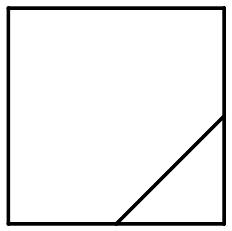
\includegraphics[width=.42\linewidth]{assets/asset-061-01.jpg}
\end{center}
\begin{choices}
  \item $346$
  \item $373$
  \item $446$
  \item $473$
\end{choices}
\begin{solution}
\textbf{答案：}B

\textbf{分析：}通过做辅助线，将已知所求量转化到一个三角形中，借助正弦定理，求得 $A'B'$，进而得到答案．

\textbf{详解：}过 $C$ 作 $CH \perp BB'$，过 $B$ 作 $BD \perp AA'$，则 $AA' - CC' = AA' - (BB' - BH) = AA' - BB' + 100 = AD + 100$．由题易知 $\triangle ADB$ 为等腰直角三角形，所以 $AD = DB$，故 $AA' - CC' = DB + 100 = A'B' + 100$．因为 $\angle BCH = 15^\circ$，所以 $CH = C'B' = \frac{100}{\tan 15^\circ}$．在 $\triangle A'B'C'$ 中，由正弦定理得 $\frac{A'B'}{\sin 45^\circ} = \frac{C'B'}{\sin 75^\circ} = \frac{100}{\tan 15^\circ \cos 15^\circ \sin 15^\circ}$，而 $\sin 15^\circ = \frac{\sqrt{6}-\sqrt{2}}{4}$，得 $A'B' = 100(\sqrt{3}+1) \approx 273$，所以 $AA' - CC' \approx 373$．
\end{solution}
\end{question}

\begin{question}[points=5]
\textbf{来源：}2021 年 全国甲卷-理科，第 14 题\par
已知向量 $\vec{a} = (3,1)$, $\vec{b} = (1,0)$, $\vec{c} = \vec{a} + k\vec{b}$．若 $\vec{a} \perp \vec{c}$，则 $k = $ ．
\fillin[{$-\frac{10}{3}$}]
\begin{solution}
\textbf{答案：}$-\frac{10}{3}$

\textbf{分析：}利用向量的坐标运算法则求得向量 $\vec{c}$ 的坐标，利用向量的数量积为零求得 $k$ 的值．

\textbf{详解：}$\vec{c} = (3+k, 1)$，由 $\vec{a} \perp \vec{c}$ 得 $3(3+k) + 1\times 1 = 0$，解得 $k = -\frac{10}{3}$．
\end{solution}
\end{question}

\begin{question}[points=5]
\textbf{来源：}2021 年 全国甲卷-文科，第 8 题\par
在 $\triangle ABC$ 中，已知 $B=120^{\circ}$, $AC=\sqrt{19}$, $AB=2$, 则 $BC=$ ( )
\begin{choices}
  \item 1
  \item $\sqrt{2}$
  \item $\sqrt{5}$
  \item 3
\end{choices}
\begin{solution}
\textbf{答案：}D

\textbf{分析：}利用余弦定理得到关于 $BC$ 长度的方程，解方程即可求得边长.

\textbf{详解：}设 $AB=c$, $AC=b$, $BC=a$, 结合余弦定理：$b^2 = a^2 + c^2 - 2ac \cos B$ 可得：$19 = a^2 + 4 - 2 \times a \times \cos 120^{\circ}$, 即 $a^2 + 2a -15 = 0$, 解得 $a=3$（$a=-5$ 舍去），故 $BC=3$.
\end{solution}
\end{question}

\begin{question}[points=5]
\textbf{来源：}2021 年 全国甲卷-文科，第 13 题\par
若向量 $\vec{a}, \vec{b}$ 满足 $|\vec{a}|=3$, $|\vec{a}-\vec{b}|=5$, $\vec{a}\cdot\vec{b}=1$, 则 $|\vec{b}|=$ .
\fillin[{$3\sqrt{2}$}]
\begin{solution}
\textbf{答案：}$3\sqrt{2}$

\textbf{分析：}根据题目条件，利用 $|\vec{a}-\vec{b}|$ 模的平方可以得出答案.

\textbf{详解：}因为 $|\vec{a}-\vec{b}|=5$, 所以 $|\vec{a}-\vec{b}|^2 = |\vec{a}|^2 + |\vec{b}|^2 - 2\vec{a}\cdot\vec{b} = 9 + |\vec{b}|^2 - 2 = 25$, 所以 $|\vec{b}|^2 = 18$, $|\vec{b}| = 3\sqrt{2}$.
\end{solution}
\end{question}

\begin{question}[points=5]
\textbf{来源：}2021 年 全国乙卷-理科，第 9 题\par
魏晋时期刘徽撰写的《海岛算经》是关于测量的数学著作，其中第一题是测量海岛的高。如图，点$E,H,G$在水平线$AC$上，$DE$和$FG$是两个垂直于水平面且等高的测量标杆的高度，称为“表高”，$EG$称为“表距”，$GC$和$EH$都称为“表目距”，$GC$与$EH$的差称为“表目距的差”。则海岛的高$AB=$（  ）
\begin{choices}
  \item $\frac{\text{表高}\times\text{表距}}{\text{表目距的差}}+\text{表高}$
  \item $\frac{\text{表高}\times\text{表距}}{\text{表目距的差}}-\text{表高}$
  \item $\frac{\text{表高}\times\text{表距}}{\text{表目距的差}}+\text{表距}$
  \item $\frac{\text{表高}\times\text{表距}}{\text{表目距的差}}-\text{表距}$
\end{choices}
\begin{solution}
\textbf{答案：}$\frac{\text{表高}\times\text{表距}}{\text{表目距的差}}+\text{表高}$

\textbf{详解：}连接$DF$交$AB$于$M$，则$AB=AM+BM$。记$\angle BDM=\alpha$，$\angle BFM=\beta$，则$\frac{MB}{\tan\beta}-\frac{MB}{\tan\alpha}=MF-MD=DF$。而$\tan\beta=\frac{FG}{GC}$，$\tan\alpha=\frac{ED}{EH}$。所以$MB\left(\frac{1}{\tan\beta}-\frac{1}{\tan\alpha}\right)=MB\cdot\left(\frac{GC}{FG}-\frac{EH}{ED}\right)=MB\cdot\frac{GC-EH}{ED}$。故$MB=\frac{ED\cdot DF}{GC-EH}=\frac{\text{表高}\times\text{表距}}{\text{表目距的差}}$，所以高$AB=\frac{\text{表高}\times\text{表距}}{\text{表目距的差}}+\text{表高}$。故选A。
\end{solution}
\end{question}

\begin{question}[points=5]
\textbf{来源：}2021 年 全国乙卷-理科，第 14 题\par
已知向量$\vec{a}=(1,3)$，$\vec{b}=(3,4)$，若$(\vec{a}-\lambda\vec{b})\perp\vec{b}$，则$\lambda=$。
\fillin[{$\frac{3}{5}$}]
\begin{solution}
\textbf{答案：}$\frac{3}{5}$

\textbf{详解：}由题意得$(\vec{a}-\lambda\vec{b})\cdot\vec{b}=0$，即$15-25\lambda=0$，解得$\lambda=\frac{3}{5}$。
\end{solution}
\end{question}

\begin{question}[points=5]
\textbf{来源：}2021 年 全国乙卷-理科，第 15 题\par
记$\triangle ABC$的内角$A$，$B$，$C$的对边分别为$a$，$b$，$c$，面积为$\sqrt{3}$，$B=60^\circ$，$a^2+c^2=3ac$，则$b=$。
\fillin[{$2\sqrt{2}$}]
\begin{solution}
\textbf{答案：}$2\sqrt{2}$

\textbf{详解：}$S_{\triangle ABC}=\frac12ac\sin B=\frac{\sqrt{3}}{4}ac=\sqrt{3}$，所以$ac=4$，由余弦定理，$b^2=a^2+c^2-2ac\cos B=3ac-ac=2ac=8$，所以$b=2\sqrt{2}$。
\end{solution}
\end{question}

\begin{question}[points=5]
\textbf{来源：}2021 年 全国乙卷-文科，第 13 题\par
已知向量 $\vec{a} = (2,5)$ ， $\vec{b} = (\lambda, 4)$ ，若 $\vec{a} // \vec{b}$ ，则 $\lambda =$ .
\fillin[{$\frac{8}{5}$}]
\begin{solution}
\textbf{答案：}$\frac{8}{5}$

\textbf{分析：}由已知 $\vec{a} // \vec{b}$ 可得 $2 \times 4 = 5\lambda \Rightarrow \lambda = \frac{8}{5}$ .
\end{solution}
\end{question}

\begin{question}[points=5]
\textbf{来源：}2021 年 全国乙卷-文科，第 15 题\par
记 $\triangle ABC$ 的内角 $A$ ， $B$ ， $C$ 的对边分别为 $a$ ， $b$ ， $c$ ，面积为 $\sqrt{3}$ ， $B = 60^\circ$ ， $a^2 + c^2 = 3ac$ ，则 $b =$ .
\fillin[{$2\sqrt{2}$}]
\begin{solution}
\textbf{答案：}$2\sqrt{2}$

\textbf{分析：}由面积公式 $S = \frac{1}{2}ac\sin B = \sqrt{3}$ ，且 $B = 60^\circ$ ，解得 $ac = 4$ ，
又由余弦定理 $b^2 = a^2 + c^2 - 2ac\cos B$ ， $a^2 + c^2 = 3ac$ ，且 $b > 0$ ，
解得 $b = 2\sqrt{2}$ .
\end{solution}
\end{question}

\begin{question}[points=5]
\textbf{来源：}2021 年 上海春季卷，第 16 题\par
在 $\triangle ABC$ 中，$D$ 为 $BC$ 中点，$E$ 为 $AD$ 中点，则以下结论：①存在 $\triangle ABC$，使得 $\overrightarrow{AB}\cdot\overrightarrow{CE}=0$；②存在三角形 $\triangle ABC$，使得 $\overrightarrow{CE}//(\overrightarrow{CB}+\overrightarrow{CA})$；它们的成立情况是 (\_\_\_\_\_\_\_\_\_\_)
\begin{choices}
  \item ①成立，②成立
  \item ①成立，②不成立
  \item ①不成立，②成立
  \item ①不成立，②不成立
\end{choices}
\begin{solution}
\textbf{答案：}B

\textbf{分析：}设 $A(2x,2y)$，$B(-1,0)$，$C(1,0)$，$D(0,0)$，$E(x,y)$，由向量数量积的坐标运算即可判断①；$F$ 为 $AB$ 中点，可得 $(\overrightarrow{CB}+\overrightarrow{CA})=2\overrightarrow{CF}$，由 $D$ 为 $BC$ 中点，可得 $CF$ 与 $AD$ 的交点即为重心 $G$，从而可判断②．

\textbf{详解：}不妨设 $A(2x,2y)$，$B(-1,0)$，$C(1,0)$，$D(0,0)$，$E(x,y)$，① $\overrightarrow{AB}=(-1-2x,-2y)$，$\overrightarrow{CE}=(x-1,y)$，若 $\overrightarrow{AB}\cdot\overrightarrow{CE}=0$，则 $-(1+2x)(x-1)-2y^2=0$，即 $-(1+2x)(x-1)=2y^2$，满足条件的 $(x,y)$ 存在，例如 $(0,\frac{\sqrt{2}}{2})$，满足上式，所以①成立；② $F$ 为 $AB$ 中点，$(\overrightarrow{CB}+\overrightarrow{CA})=2\overrightarrow{CF}$，$CF$ 与 $AD$ 的交点即为重心 $G$，因为 $G$ 为 $AD$ 的三等分点，$E$ 为 $AD$ 中点，所以 $\overrightarrow{CE}$ 与 $\overrightarrow{CG}$ 不共线，即②不成立．故选B．
\end{solution}
\end{question}

\begin{question}[points=14]
\textbf{来源：}2021 年 上海春季卷，第 18 题\par
已知 $A$、$B$、$C$ 为 $\triangle ABC$ 的三个内角，$a$、$b$、$c$ 是其三条边，$a=2$，$\cos C=-\frac{1}{4}$．\begin{enumerate}\item[(1)] 若 $\sin A=2\sin B$，求 $b$、$c$；\item[(2)] 若 $\cos(A-\frac{\pi}{4})=\frac{4}{5}$，求 $c$．\end{enumerate}
\begin{solution}
\textbf{答案：}$(1)\ b=1,\ c=\sqrt{6}$；$(2)\ c=\frac{5\sqrt{30}}{2}$

\textbf{分析：}（1）由已知利用正弦定理即可求解 $b$ 的值；利用余弦定理即可求解 $c$ 的值．\newline（2）根据已知利用两角差的余弦公式，同角三角函数基本关系式可求得 $\cos A$，$\sin A$，$\sin C$ 的值，进而根据正弦定理可得 $c$ 的值．

\textbf{详解：}（1）因为 $\sin A=2\sin B$，可得 $a=2b$，又 $a=2$，可得 $b=1$，由余弦定理 $\cos C=\frac{a^2+b^2-c^2}{2ab}=\frac{2^2+1^2-c^2}{2\times 2\times 1}=-\frac{1}{4}$，解得 $c=\sqrt{6}$．\newline（2）因为 $\cos(A-\frac{\pi}{4})=\frac{\sqrt{2}}{2}(\cos A+\sin A)=\frac{4}{5}$，可得 $\cos A+\sin A=\frac{4\sqrt{2}}{5}$，又 $\cos^2 A+\sin^2 A=1$，解得 $\cos A=\frac{7\sqrt{2}}{10},\sin A=\frac{\sqrt{2}}{10}$ 或 $\sin A=\frac{7\sqrt{2}}{10},\cos A=\frac{\sqrt{2}}{10}$，因为 $\cos C=-\frac{1}{4}$，可得 $\sin C=\frac{\sqrt{15}}{4}$，$\tan C=-\sqrt{15}$，若 $\sin A=\frac{7\sqrt{2}}{10}$，$\cos A=\frac{\sqrt{2}}{10}$，可得 $\tan A=7$，则 $\tan B=-\tan(A+C)=\frac{\tan A+\tan C}{\tan A\tan C-1}=\frac{7-\sqrt{15}}{7\times(-\sqrt{15})-1}<0$，可得 $B$ 为钝角，这与 $C$ 为钝角矛盾，舍去，所以 $\sin A=\frac{\sqrt{2}}{10}$，由正弦定理 $\frac{a}{\sin A}=\frac{c}{\sin C}$，可得 $c=\frac{5\sqrt{30}}{2}$．
\end{solution}
\end{question}

\begin{question}[points=4]
\textbf{来源：}2021 年 上海卷，第 4 题\par
如图边长为3的正方形$ABCD$, 则$\overrightarrow{AB}\cdot\overrightarrow{AC}=$．
\fillin[{$9$}]
\begin{solution}
\textbf{答案：}$9$

\textbf{分析：}利用向量投影转化到边上.

\textbf{详解：}方法一：$\overrightarrow{AB}\cdot\overrightarrow{AC}=|\overrightarrow{AB}|^2=9$；方法二：由已知$|\overrightarrow{AB}|=3$，$|\overrightarrow{AC}|=3\sqrt{2}$，$\langle\overrightarrow{AC},\overrightarrow{AB}\rangle=\frac{\pi}{4}$，则$\overrightarrow{AB}\cdot\overrightarrow{AC}=3\times3\sqrt{2}\times\frac{\sqrt{2}}{2}=9$
\end{solution}
\end{question}

\begin{question}[points=14]
\textbf{来源：}2021 年 上海卷，第 18 题\par
在$\triangle ABC$中，已知$a=3, b=2c$（1)若$\angle A=\frac{2\pi}{3}$, 求$\triangle ABC$的面积；（2)若$2\sin B-\sin C=1$,求$\triangle ABC$的周长.
\begin{solution}
\textbf{答案：}(1)$\frac{9\sqrt{3}}{14}$；(2)$3+4\sqrt{2}\pm\sqrt{5}$

\textbf{分析：}（1）由已知利用余弦定理即可求解$b$，$c$的值；再利用面积公式求$\triangle ABC$的面积．（2）根据$b=2c$与$2\sin B-\sin C=1$建立关于角度的三角方程，求解$\sin C$, $\sin B$的值，再求$\sin A$，则根据正弦定理以及$a=3$，则三边可求．

\textbf{详解：}（1)$\cos A=\frac{b^2+c^2-a^2}{2bc}\Rightarrow\frac{(2c)^2+c^2-3^2}{2\times(2c)c}=-\frac{1}{2}\Rightarrow c=\frac{3\sqrt{7}}{7}$, $b=\frac{6\sqrt{7}}{7}$；$S_{\triangle ABC}=\frac{1}{2}bc\sin A=\frac{1}{2}\times2c^2\times\sin\frac{2\pi}{3}=\frac{1}{2}\times2\times(\frac{3\sqrt{7}}{7})^2\times\frac{\sqrt{3}}{2}=\frac{9\sqrt{3}}{14}$（2）$b=2c\Rightarrow\sin B=2\sin C\Rightarrow2\times2\sin C-\sin C=1\Rightarrow\sin C=\frac{1}{3}$, $\sin B=\frac{2}{3}$，$\sin A=\sin(B+C)=\sin B\cos C+\cos B\sin C=\frac{4\sqrt{2}\pm5}{9}$，$c=\frac{a\sin C}{\sin A}=\frac{4\sqrt{2}\pm5}{3}$，三角形周长$l=a+b+c=a+3c=3+4\sqrt{2}\pm\sqrt{5}$
\end{solution}
\end{question}

\begin{question}[points=5]
\textbf{来源：}2021 年 天津卷，第 15 题\par
在边长为1的等边三角形 $ABC$ 中，$D$ 为线段 $BC$ 上的动点，$DE \perp AB$ 且交 $AB$ 于点 $E$，$DF // AB$ 且交 $AC$ 于点 $F$，则 $|2\overrightarrow{BE} + \overrightarrow{DF}|$ 的值为；$(\overrightarrow{DE} + \overrightarrow{DF}) \cdot \overrightarrow{DA}$ 的最小值为.
\fillin[{$1$；$\frac{11}{20}$}]
\begin{solution}
\textbf{答案：}$1$；$\frac{11}{20}$

\textbf{分析：}设 $BE = x$，由 $(2\overrightarrow{BE} + \overrightarrow{DF})^2$ 可求出；将 $(\overrightarrow{DE} + \overrightarrow{DF}) \cdot \overrightarrow{DA}$ 化为关于 $x$ 的关系式即可求出最值.

\textbf{详解：}设 $BE = x$，$x \in (0, \frac{1}{2})$，则 $BD=2x$，$DE=\sqrt{3}x$，$DC=1-2x$，$\triangle DFC$ 为等边三角形，边长为 $1-2x$，$DE \perp DF$，则 $(2\overrightarrow{BE} + \overrightarrow{DF})^2 = 4x^2 + 4x(1-2x)\cos 0^\circ + (1-2x)^2 = 1$，所以 $|2\overrightarrow{BE} + \overrightarrow{DF}|=1$；$(\overrightarrow{DE}+\overrightarrow{DF})\cdot\overrightarrow{DA} = (\overrightarrow{DE}+\overrightarrow{DF})\cdot(\overrightarrow{DE}+\overrightarrow{EA}) = \overrightarrow{DE}^2 + \overrightarrow{DF}\cdot\overrightarrow{EA} = (\sqrt{3}x)^2 + (1-2x)(1-x) = 5x^2 -3x+1 = 5\left(x-\frac{3}{10}\right)^2 + \frac{11}{20}$，所以当 $x=\frac{3}{10}$ 时，最小值为 $\frac{11}{20}$.
\end{solution}
\end{question}

\begin{question}[points=14]
\textbf{来源：}2021 年 天津卷，第 16 题\par
在 $\triangle ABC$，角 $A, B, C$ 所对的边分别为 $a, b, c$，已知 $\sin A : \sin B : \sin C = 2 : 1 : \sqrt{2}$，$b = \sqrt{2}$．

（I）求 $a$ 的值；

（II）求 $\cos C$ 的值；

（III）求 $\sin\left(2C - \frac{\pi}{6}\right)$ 的值．
\begin{solution}
\textbf{答案：}$a=2\sqrt{2}$；$\cos C = \frac{3}{4}$；$\frac{3\sqrt{21}-1}{16}$

\textbf{分析：}（I）由正弦定理可得 $a:b:c = 2:1:\sqrt{2}$，即可求出；
（II）由余弦定理即可计算；
（III）利用二倍角公式求出 $2C$ 的正弦值和余弦值，再由两角差的正弦公式即可求出.

\textbf{详解：}（I）由正弦定理得 $a:b:c = 2:1:\sqrt{2}$，$\because b = \sqrt{2}$，$\therefore a = 2\sqrt{2}$，$c=2$；
（II）$\cos C = \frac{a^2+b^2-c^2}{2ab} = \frac{8+2-4}{2\times 2\sqrt{2}\times \sqrt{2}} = \frac{6}{8} = \frac{3}{4}$；
（III）$\because \cos C = \frac{3}{4}$，$\therefore \sin C = \frac{\sqrt{7}}{4}$，$\sin 2C = 2\sin C \cos C = \frac{3\sqrt{7}}{8}$，$\cos 2C = 2\cos^2 C -1 = \frac{9}{8}-1 = \frac{1}{8}$，$\sin\left(2C - \frac{\pi}{6}\right) = \sin 2C \cos \frac{\pi}{6} - \cos 2C \sin \frac{\pi}{6} = \frac{3\sqrt{7}}{8} \times \frac{\sqrt{3}}{2} - \frac{1}{8} \times \frac{1}{2} = \frac{3\sqrt{21} - 1}{16}$.
\end{solution}
\end{question}

\begin{question}[points=5]
\textbf{来源：}2021 年 新高考II卷，第 15 题\par
已知向量$\vec{a}+\vec{b}+\vec{c}=\vec{0}$，$|\vec{a}|=1$，$|\vec{b}|=|\vec{c}|=2$，$\vec{a}\cdot\vec{b}+\vec{b}\cdot\vec{c}+\vec{c}\cdot\vec{a}=$．
\fillin[{$-\frac{9}{2}$}]
\begin{solution}
\textbf{答案：}$-\frac{9}{2}$

\textbf{分析：}由已知可得$(\vec{a}+\vec{b}+\vec{c})^2=0$，展开化简后可得结果.

\textbf{详解：}由已知可得$(\vec{a}+\vec{b}+\vec{c})^2=|\vec{a}|^2+|\vec{b}|^2+|\vec{c}|^2+2(\vec{a}\cdot\vec{b}+\vec{b}\cdot\vec{c}+\vec{c}\cdot\vec{a})=9+2(\vec{a}\cdot\vec{b}+\vec{b}\cdot\vec{c}+\vec{c}\cdot\vec{a})=0$，因此$\vec{a}\cdot\vec{b}+\vec{b}\cdot\vec{c}+\vec{c}\cdot\vec{a}=-\frac{9}{2}$.故答案为：$-\frac{9}{2}$.
\end{solution}
\end{question}

\begin{question}[points=12]
\textbf{来源：}2021 年 新高考II卷，第 18 题\par
在$\triangle ABC$中，角$A$、$B$、$C$所对的边长分别为$a$、$b$、$c$，$b=a+1$，$c=a+2$．

（1）若$2\sin C=3\sin A$，求$\triangle ABC$的面积；

（2）是否存在正整数$a$，使得$\triangle ABC$为钝角三角形?若存在，求出$a$的值；若不存在，说明理由．
\begin{solution}
\textbf{答案：}(1) $\frac{15\sqrt{7}}{4}$；(2) 存在，且$a=2$.

\textbf{分析：}(1)由正弦定理可得出$2c=3a$，结合已知条件求出$a$的值，进一步可求得$b$、$c$的值，利用余弦定理以及同角三角函数的基本关系求出$\sin B$，再利用三角形的面积公式可求得结果； (2)分析可知，角$C$为钝角，由$\cos C<0$结合三角形三边关系可求得整数$a$的值.

\textbf{详解：}(1)因为$2\sin C=3\sin A$，则$2c=2(a+2)=3a$，则$a=4$，故$b=5$，$c=6$，$\cos C=\frac{a^2+b^2-c^2}{2ab}=\frac{1}{8}$，所以$C$为锐角，则$\sin C=\sqrt{1-\cos^2 C}=\frac{3\sqrt{7}}{8}$，因此$S_{\triangle ABC}=\frac{1}{2}ab\sin C=\frac{1}{2}\times4\times5\times\frac{3\sqrt{7}}{8}=\frac{15\sqrt{7}}{4}$； (2)显然$c>b>a$，若$\triangle ABC$为钝角三角形，则$C$为钝角，由余弦定理可得$\cos C=\frac{a^2+b^2-c^2}{2ab}=\frac{a^2+(a+1)^2-(a+2)^2}{2a(a+1)}=\frac{a^2-2a-3}{2a(a+1)}<0$，解得$-1<a<3$，则$0<a<3$，由三角形三边关系可得$a+a+1>a+2$，可得$a>1$，$\because a\in\mathbb{Z}$，故$a=2$.
\end{solution}
\end{question}

\begin{question}[points=5]
\textbf{来源：}2021 年 新高考I卷，第 10 题\par
已知 $O$ 为坐标原点, 点 $P_1(\cos\alpha, \sin\alpha)$, $P_2(\cos\beta, -\sin\beta)$, $P_3(\cos(\alpha+\beta), \sin(\alpha+\beta))$, $A(1,0)$, 则 ( )
\begin{choices}
  \item $|\overrightarrow{OP_1}| = |\overrightarrow{OP_2}|$
  \item $|\overrightarrow{AP_1}| = |\overrightarrow{AP_2}|$
  \item $\overrightarrow{OA} \cdot \overrightarrow{OP_3} = \overrightarrow{OP_1} \cdot \overrightarrow{OP_2}$
  \item $\overrightarrow{OA} \cdot \overrightarrow{OP_1} = \overrightarrow{OP_2} \cdot \overrightarrow{OP_3}$
\end{choices}
\begin{solution}
\textbf{答案：}A, C

\textbf{分析：}A、B写出向量坐标, 利用坐标公式求模; C、D应用向量数量积的坐标表示及两角和差公式化简.

\textbf{详解：}A: $\overrightarrow{OP_1} = (\cos\alpha, \sin\alpha)$, $\overrightarrow{OP_2} = (\cos\beta, -\sin\beta)$, $|\overrightarrow{OP_1}| = \sqrt{\cos^2\alpha + \sin^2\alpha} = 1$, $|\overrightarrow{OP_2}| = 1$, 故正确; B: $|\overrightarrow{AP_1}| = \sqrt{(\cos\alpha-1)^2 + \sin^2\alpha} = \sqrt{2(1-\cos\alpha)} = 2|\sin\frac{\alpha}{2}|$, $|\overrightarrow{AP_2}| = 2|\sin\frac{\beta}{2}|$, 不一定相等, 错误; C: $\overrightarrow{OA} \cdot \overrightarrow{OP_3} = \cos(\alpha+\beta)$, $\overrightarrow{OP_1} \cdot \overrightarrow{OP_2} = \cos\alpha\cos\beta + \sin\alpha(-\sin\beta) = \cos(\alpha+\beta)$, 正确; D: $\overrightarrow{OA} \cdot \overrightarrow{OP_1} = \cos\alpha$, $\overrightarrow{OP_2} \cdot \overrightarrow{OP_3} = \cos\beta\cos(\alpha+\beta) + (-\sin\beta)\sin(\alpha+\beta) = \cos(\alpha+2\beta)$, 不一定相等, 错误. 故选AC.
\end{solution}
\end{question}

\begin{question}[points=12]
\textbf{来源：}2021 年 新高考I卷，第 19 题\par
记 $\triangle ABC$ 的内角 $A$, $B$, $C$ 的对边分别为 $a$, $b$, $c$. 已知 $b^2 = ac$, 点 $D$ 在边 $AC$ 上, $BD \sin\angle ABC = a \sin C$.

(1) 证明: $BD = b$;

(2) 若 $AD = 2DC$, 求 $\cos\angle ABC$.
\begin{solution}
\textbf{答案：}(1) 证明见解析; (2) $\cos\angle ABC = \frac{7}{12}$

\textbf{分析：}(1) 利用正弦定理的边角关系得到 $BD = \frac{ac}{b}$, 结合 $b^2 = ac$ 得证. (2) 由题设及余弦定理, 利用 $\angle ADB + \angle CDB = \pi$ 建立方程, 解出 $a,b,c$ 关系, 再求余弦值.

\textbf{详解：}(1) 由正弦定理, $\frac{a}{\sin\angle ABC} = \frac{c}{\sin C}$, 故 $\frac{\sin C}{\sin\angle ABC} = \frac{c}{a}$. 又 $BD = \frac{a\sin C}{\sin\angle ABC}$, 所以 $BD = \frac{ac}{b}$. 因为 $b^2 = ac$, 所以 $BD = b$.
(2) 设 $BD = b$, $AD = \frac{2b}{3}$, $DC = \frac{b}{3}$. 在 $\triangle ABD$ 和 $\triangle CBD$ 中分别应用余弦定理, 并利用 $\cos\angle ADB = -\cos\angle CDB$, 可得 $2a^2 + c^2 = \frac{11b^2}{3}$. 结合 $b^2 = ac$, 解得 $\frac{a^2}{b^2} = \frac{1}{3}$ 或 $\frac{3}{2}$. 当 $\frac{a^2}{b^2} = \frac{1}{3}$ 时, $\cos\angle ABC = \frac{a^2 + c^2 - b^2}{2ac} = \frac{7}{6} > 1$, 舍去; 当 $\frac{a^2}{b^2} = \frac{3}{2}$ 时, $\cos\angle ABC = \frac{7}{12}$, 符合题意.
\end{solution}
\end{question}

\begin{question}[points=6]
\textbf{来源：}2021 年 浙江卷，第 14 题\par
在 $\triangle ABC$ 中, $\angle B = 60^\circ$, $AB=2$, $M$ 是 $BC$ 的中点, $AM=2\sqrt{3}$, 则 $AC=$ ，$\cos\angle MAC=$ .
\fillin[{$2\sqrt{13}$; $\frac{2\sqrt{39}}{13}$}]
\begin{solution}
\textbf{答案：}$2\sqrt{13}$; $\frac{2\sqrt{39}}{13}$

\textbf{分析：}由余弦定理求得 $BC$, 再由余弦定理可得 $AC$ 和 $\cos\angle MAC$.

\textbf{详解：}在 $\triangle ABM$ 中, 由余弦定理: $12=4+BM^2-2\cdot2\cdot BM\cdot\frac12$, 解得 $BM=4$, 则 $BC=8$. 在 $\triangle ABC$ 中, $AC^2=4+64-2\cdot2\cdot8\cdot\frac12=52$, 所以 $AC=2\sqrt{13}$. 在 $\triangle AMC$ 中, $\cos\angle MAC = \frac{AC^2+AM^2-MC^2}{2\cdot AM\cdot AC} = \frac{52+12-16}{2\cdot2\sqrt{3}\cdot2\sqrt{13}} = \frac{48}{8\sqrt{39}} = \frac{2\sqrt{39}}{13}$.
\end{solution}
\end{question}

\begin{question}[points=4]
\textbf{来源：}2021 年 浙江卷，第 17 题\par
已知平面向量 $\vec{a},\vec{b},\vec{c}$ $(\vec{c}\neq\vec{0})$ 满足 $|\vec{a}|=1$, $|\vec{b}|=2$, $\vec{a}\cdot\vec{b}=0$, $(\vec{a}-\vec{b})\cdot\vec{c}=0$. 记向量 $\vec{d}$ 在 $\vec{a},\vec{b}$ 方向上的投影分别为 $x,y$, $\vec{d}-\vec{a}$ 在 $\vec{c}$ 方向上的投影为 $z$, 则 $x^2+y^2+z^2$ 的最小值为.
\fillin[{$\frac{2}{5}$}]
\begin{solution}
\textbf{答案：}$\frac{2}{5}$

\textbf{分析：}设 $\vec{a}=(1,0)$, $\vec{b}=(0,2)$, $\vec{c}=(m,n)$, 由条件得 $m=2n$, 再由投影公式得 $2x+y\pm\sqrt{5}z=2$, 利用柯西不等式求最小值.

\textbf{详解：}令 $\vec{a}=(1,0)$, $\vec{b}=(0,2)$, $\vec{c}=(2n,n)$, 设 $\vec{d}=(x,y)$, 则 $z = \frac{(\vec{d}-\vec{a})\cdot\vec{c}}{|\vec{c}|} = \frac{2n(x-1)+ny}{\sqrt{5}n} = \frac{2x+y-2}{\sqrt{5}}$, 故 $2x+y-\sqrt{5}z=2$. 由柯西不等式: $(2^2+1^2+(\sqrt{5})^2)(x^2+y^2+z^2) \geq (2x+y-\sqrt{5}z)^2=4$, 所以 $x^2+y^2+z^2 \geq \frac{4}{10}=\frac{2}{5}$, 等号当 $\frac{x}{2}=\frac{y}{1}=\frac{z}{-\sqrt{5}}$ 时取得, 即 $x=\frac{4}{5},y=\frac{2}{5},z=-\frac{2\sqrt{5}}{5}$.
\end{solution}
\end{question}

\section*{2022 年}

\begin{question}[points=4]
\textbf{来源：}2022 年 北京卷，第 10 题\par
在 $\triangle ABC$ 中，$AC = 3, BC = 4, \angle C = 90^\circ$。$P$ 为 $\triangle ABC$ 所在平面内的动点，且 $PC = 1$，则 $\overrightarrow{PA} \cdot \overrightarrow{PB}$ 的取值范围是
\begin{choices}
  \item $[-5,3]$
  \item $[-3,5]$
  \item $[-6,4]$
  \item $[-4,6]$
\end{choices}
\begin{solution}
\textbf{答案：}D

\textbf{分析：}依题意建立平面直角坐标系，设 $P(\cos\theta,\sin\theta)$，表示出 $\overrightarrow{PA}$，$\overrightarrow{PB}$，根据数量积的坐标表示、辅助角公式及正弦函数的性质计算。

\textbf{详解：}解：依题意如图建立平面直角坐标系，则 $C(0,0)$，$A(3,0)$，$B(0,4)$，因为 $PC=1$，所以 $P$ 在以 $C$ 为圆心，1为半径的圆上运动，设 $P(\cos\theta,\sin\theta)$，$\theta \in [0,2\pi)$。
$\overrightarrow{PA} = (3-\cos\theta, -\sin\theta)$，$\overrightarrow{PB} = (-\cos\theta, 4-\sin\theta)$，
$\overrightarrow{PA} \cdot \overrightarrow{PB} = (-\cos\theta)(3-\cos\theta) + (4-\sin\theta)(-\sin\theta)$
$= \cos^2\theta - 3\cos\theta - 4\sin\theta + \sin^2\theta$
$= 1 - 3\cos\theta - 4\sin\theta$
$= 1 - 5\sin(\theta + \varphi)$，其中 $\sin\varphi = \dfrac{3}{5}$，$\cos\varphi = \dfrac{4}{5}$。
因为 $-1 \leq \sin(\theta + \varphi) \leq 1$，所以 $-4 \leq 1 - 5\sin(\theta + \varphi) \leq 6$，即 $\overrightarrow{PA} \cdot \overrightarrow{PB} \in [-4,6]$。故选D。
\end{solution}
\end{question}

\begin{question}[points=13]
\textbf{来源：}2022 年 北京卷，第 16 题\par
在 $\triangle ABC$ 中，$\sin 2C = \sqrt{3} \sin C$。

（1）求 $\angle C$；

（2）若 $b=6$，且 $\triangle ABC$ 的面积为 $6\sqrt{3}$，求 $\triangle ABC$ 的周长。
\begin{solution}
\textbf{答案：}（1）$\dfrac{\pi}{6}$；（2）$6+6\sqrt{3}$

\textbf{分析：}（1）利用二倍角的正弦公式化简可得 $\cos C$ 的值，结合角 $C$ 的取值范围可求得角 $C$ 的值；（2）利用三角形的面积公式可求得 $a$ 的值，由余弦定理可求得 $c$ 的值，即可求得周长。

\textbf{详解：}（1）解：因为 $C\in(0,\pi)$，则 $\sin C>0$，由已知可得 $\sqrt{3}\sin C = 2\sin C\cos C$，可得 $\cos C = \dfrac{\sqrt{3}}{2}$，因此 $C=\dfrac{\pi}{6}$。
（2）解：由三角形的面积公式 $S_{\triangle ABC} = \dfrac{1}{2}ab\sin C = \dfrac{1}{2}a\cdot 6\cdot \dfrac{1}{2} = 6\sqrt{3}$，解得 $a=4\sqrt{3}$。由余弦定理得 $c^2 = a^2+b^2-2ab\cos C = 48+36-2\times 4\sqrt{3}\times 6\times \dfrac{\sqrt{3}}{2} = 12$，$\therefore c=2\sqrt{3}$。所以 $\triangle ABC$ 的周长为 $a+b+c = 4\sqrt{3}+6+2\sqrt{3} = 6+6\sqrt{3}$。
\end{solution}
\end{question}

\begin{question}[points=5]
\textbf{来源：}2022 年 全国甲卷-理科，第 13 题\par
设向量 $\vec{a}$, $\vec{b}$ 的夹角的余弦值为 $\frac{1}{3}$，且 $|\vec{a}|=1$，$|\vec{b}|=3$，则 $(2\vec{a}+\vec{b})\cdot\vec{b}=$ ．
\fillin[{$11$}]
\begin{solution}
\textbf{答案：}$11$

\textbf{分析：}设$\vec{a}$与$\vec{b}$的夹角为$\theta$，依题意可得$\cos\theta=\frac{1}{3}$，再根据数量积的定义求出$\vec{a}\cdot\vec{b}$，最后根据数量积的运算律计算可得.

\textbf{详解：}解：设$\vec{a}$与$\vec{b}$的夹角为$\theta$，因为$\vec{a}$与$\vec{b}$的夹角的余弦值为$\frac{1}{3}$，即$\cos\theta=\frac{1}{3}$，又$|\vec{a}|=1$, $|\vec{b}|=3$，所以$\vec{a}\cdot\vec{b}=|\vec{a}||\vec{b}|\cos\theta=1\times3\times\frac{1}{3}=1$，所以$(2\vec{a}+\vec{b})\cdot\vec{b}=2\vec{a}\cdot\vec{b}+|\vec{b}|^2=2\times1+3^2=11$. 故答案为11.
\end{solution}
\end{question}

\begin{question}[points=5]
\textbf{来源：}2022 年 全国甲卷-理科，第 16 题\par
已知 $\triangle ABC$ 中，点D在边BC上，$\angle ADB=120^\circ$, $AD=2$, $CD=2BD$. 当 $\frac{AC}{AB}$ 取得最小值时，$BD=$ ．
\fillin[{$\sqrt{3}-1$}]
\begin{solution}
\textbf{答案：}$\sqrt{3}-1$

\textbf{分析：}设$CD=2BD=2m>0$，利用余弦定理表示出$\frac{AC^2}{AB^2}$后，结合基本不等式即可得解.

\textbf{详解：}设$CD=2BD=2m>0$，则在$\triangle ABD$中，$AB^2=BD^2+AD^2-2BD\cdot AD\cos\angle ADB=m^2+4+2m$，在$\triangle ACD$中，$AC^2=CD^2+AD^2-2CD\cdot AD\cos\angle ADC=4m^2+4-4m$，所以 $\frac{AC^2}{AB^2}=\frac{4m^2+4-4m}{m^2+4+2m}=\frac{4(m^2+4+2m)-12(1+m)}{m^2+4+2m}=4-\frac{12}{m+1+\frac{3}{m+1}} \geq 4-\frac{12}{2\sqrt{3}}=4-2\sqrt{3}$，当且仅当 $m+1=\frac{3}{m+1}$ 即 $m=\sqrt{3}-1$ 时等号成立，所以当 $\frac{AC}{AB}$ 取最小值时，$m=\sqrt{3}-1$，即 $BD=\sqrt{3}-1$. 故答案为 $\sqrt{3}-1$.
\end{solution}
\end{question}

\begin{question}[points=5]
\textbf{来源：}2022 年 全国甲卷-文科，第 13 题\par
已知向量 $\vec{a}=(m,3),\vec{b}=(1,m+1)$．若 $\vec{a}\perp\vec{b}$，则 $m=$
\fillin[{$-\frac{3}{4}$}]
\begin{solution}
\textbf{答案：}$-\frac{3}{4}$
\end{solution}
\end{question}

\begin{question}[points=5]
\textbf{来源：}2022 年 全国甲卷-文科，第 16 题\par
已知 $\triangle ABC$ 中，点 $D$ 在边 $BC$ 上，$\angle ADB=120^\circ, AD=2, CD=2BD$．当 $\frac{AC}{AB}$ 取得最小值时，$BD=$
\fillin[{$\sqrt{3}-1$}]
\begin{solution}
\textbf{答案：}$\sqrt{3}-1$
\end{solution}
\end{question}

\begin{question}[points=5]
\textbf{来源：}2022 年 全国乙卷-理科，第 3 题\par
已知向量$\vec{a}, \vec{b}$满足$|\vec{a}| = 1, |\vec{b}| = \sqrt{3}, |\vec{a} - 2\vec{b}| = 3$，则$\vec{a} \cdot \vec{b} =$（\qquad）
\begin{choices}
  \item $-2$
  \item $-1$
  \item $1$
  \item $2$
\end{choices}
\begin{solution}
\textbf{答案：}C

\textbf{分析：}根据给定模长，利用向量的数量积运算求解即可.

\textbf{详解：}解：因为$|\vec{a} - 2\vec{b}|^2 = |\vec{a}|^2 - 4\vec{a} \cdot \vec{b} + 4|\vec{b}|^2$，又因为$|\vec{a}| = 1, |\vec{b}| = \sqrt{3}, |\vec{a} - 2\vec{b}| = 3$，\\所以$9 = 1 - 4\vec{a} \cdot \vec{b} + 4 \times 3 = 13 - 4\vec{a} \cdot \vec{b}$，\\所以$\vec{a} \cdot \vec{b} = 1$
\end{solution}
\end{question}

\begin{question}[points=12]
\textbf{来源：}2022 年 全国乙卷-理科，第 17 题\par
记$\triangle ABC$的内角$A,B,C$的对边分别为$a,b,c$，已知$\sin C\sin(A-B) = \sin B\sin(C-A)$．

(1)证明：$2a^2 = b^2 + c^2$；

(2)若$a=5,\cos A = \frac{25}{31}$，求$\triangle ABC$的周长．
\begin{solution}
\textbf{答案：}(1)见解析 (2)14

\textbf{分析：}(1)利用两角差的正弦公式化简，再根据正弦定理和余弦定理化角为边，从而即可得证；(2)根据(1)的结论结合余弦定理求出$bc$，从而可求得$b+c$，即可得解.

\textbf{详解：}【小问1详解】证明：因为$\sin C\sin(A-B)=\sin B\sin(C-A)$，所以$\sin C\sin A\cos B - \sin C\sin B\cos A = \sin B\sin C\cos A - \sin B\sin A\cos C$，所以$ac\cdot\frac{a^2+c^2-b^2}{2ac} - 2bc\cdot\frac{b^2+c^2-a^2}{2bc} = -ab\cdot\frac{a^2+b^2-c^2}{2ab}$，即$\frac{a^2+c^2-b^2}{2} - (b^2+c^2-a^2) = -\frac{a^2+b^2-c^2}{2}$，所以$2a^2 = b^2 + c^2$；\\【小问2详解】解：因为$a=5,\cos A=\frac{25}{31}$，由(1)得$b^2+c^2=50$，由余弦定理可得$a^2 = b^2+c^2 - 2bc\cos A$，则$50 - \frac{50}{31}bc = 25$，所以$bc = \frac{31}{2}$，故$(b+c)^2 = b^2+c^2+2bc = 50+31=81$，所以$b+c=9$，所以$\triangle ABC$的周长为$a+b+c=14$.
\end{solution}
\end{question}

\begin{question}[points=5]
\textbf{来源：}2022 年 全国乙卷-文科，第 3 题\par
已知向量 $\vec{a}=(2,1)$, $\vec{b}=(-2,4)$, 则 $|\vec{a} - \vec{b}| =$
\begin{choices}
  \item 2
  \item 3
  \item 4
  \item 5
\end{choices}
\begin{solution}
\textbf{答案：}D

\textbf{分析：}先求得 $\vec{a} - \vec{b}$, 然后求得 $|\vec{a} - \vec{b}|$.

\textbf{详解：}因为 $\vec{a} - \vec{b} = (2,1) - (-2,4) = (4,-3)$, 所以 $|\vec{a} - \vec{b}| = \sqrt{4^2 + (-3)^2} = 5$.
\end{solution}
\end{question}

\begin{question}[points=12]
\textbf{来源：}2022 年 全国乙卷-文科，第 17 题\par
记 $\triangle ABC$ 的内角 $A,B,C$ 的对边分别为 $a,b,c$, 已知 $\sin C \sin(A-B) = \sin B \sin(C-A)$.

(1) 若 $A=2B$, 求 $C$;

(2) 证明：$2a^2 = b^2 + c^2$.
\begin{solution}
\textbf{答案：}(1) $C = \frac{5\pi}{8}$; (2) 证明见解析.

\textbf{分析：}(1) 由已知和 $A=2B$ 得 $\sin C = \sin(C-A)$, 结合三角形内角和求 $C$.
(2) 展开两角差正弦，利用正弦定理和余弦定理化简.

\textbf{详解：}(1) 由 $A=2B$ 代入得 $\sin C\sin B = \sin B\sin(C-A)$, 因为 $\sin B\neq0$, 所以 $\sin C = \sin(C-A)$. 因为 $0<C<\pi$, $0<C-A<\pi$, 且 $C\neq C-A$, 所以 $C+(C-A)=\pi$, 又 $A=2B$, $A+B+C=\pi$, 解得 $C=\frac{5\pi}{8}$.
(2) 展开得 $\sin C(\sin A\cos B-\cos A\sin B) = \sin B(\sin C\cos A-\cos C\sin A)$, 由正弦定理得 $ac\cos B - bc\cos A = bc\cos A - ab\cos C$. 由余弦定理，$\frac12(a^2+c^2-b^2)-\frac12(b^2+c^2-a^2) = \frac12(b^2+c^2-a^2)-\frac12(a^2+b^2-c^2)$, 化简得 $2a^2=b^2+c^2$.
\end{solution}
\end{question}

\begin{question}[points=5]
\textbf{来源：}2022 年 上海卷，第 10 题\par
若平面向量 $|\vec{a}|=|\vec{b}|=|\vec{c}|$，且满足$\vec{a}\cdot\vec{b}=0$，$\vec{a}\cdot\vec{c}=2$，$\vec{b}\cdot\vec{c}=1$，则$|\vec{a}|=$ ．
\fillin[{$\frac{4}{5}\sqrt{5}$}]
\begin{solution}
\textbf{答案：}$\frac{4}{5}\sqrt{5}$

\textbf{分析：}利用平面向量的数量积进行分析，即可得出结果．

\textbf{详解：}解：由题意，有$\vec{a}\cdot\vec{b}=0$，则$\vec{a}\perp\vec{b}$，设$\langle\vec{a},\vec{c}\rangle=\theta$，$\vec{a}\cdot\vec{c}=|\vec{a}||\vec{c}|\cos\theta=2$①，$\vec{b}\cdot\vec{c}=|\vec{a}||\vec{c}|\cos(\frac{\pi}{2}-\theta)=|\vec{a}||\vec{c}|\sin\theta=1$②，由①÷②得$\tan\theta=2$，则$\cos\theta=\frac{\sqrt{5}}{5}$，代入①得$|\vec{a}|^2\cdot\frac{\sqrt{5}}{5}=2$，所以$|\vec{a}|^2=2\sqrt{5}$，$|\vec{a}|=\sqrt{2\sqrt{5}}=\frac{4}{5}\sqrt{5}$．故答案为：$\frac{4}{5}\sqrt{5}$．
\end{solution}
\end{question}

\begin{question}[points=5]
\textbf{来源：}2022 年 天津卷，第 14 题\par
在 $\triangle ABC$ 中，$\overrightarrow{CA}=\vec{a}$，$\overrightarrow{CB}=\vec{b}$，$D$ 是 $AC$ 中点，$\overrightarrow{CB}=2\overrightarrow{BE}$，试用 $\vec{a},\vec{b}$ 表示 $\overrightarrow{DE}$ 为，若 $\overrightarrow{AB}\perp\overrightarrow{DE}$，则 $\angle ACB$ 的最大值为
\fillin[{$\frac{3}{2}\vec{b}-\frac{1}{2}\vec{a}$ 和 $\frac{\pi}{6}$}]
\begin{solution}
\textbf{答案：}$\frac{3}{2}\vec{b}-\frac{1}{2}\vec{a}$ 和 $\frac{\pi}{6}$

\textbf{分析：}方法一：$\overrightarrow{DE}=\overrightarrow{CE}-\overrightarrow{CD}=\frac{3}{2}\vec{b}-\frac{1}{2}\vec{a}$，$\overrightarrow{AB}=\vec{b}-\vec{a}$，由 $\overrightarrow{AB}\perp\overrightarrow{DE}$ 得 $(3\vec{b}-\vec{a})\cdot(\vec{b}-\vec{a})=0$，即 $3|\vec{b}|^2+|\vec{a}|^2=4\vec{a}\cdot\vec{b}$，所以 $\cos\angle ACB=\frac{\vec{a}\cdot\vec{b}}{|\vec{a}||\vec{b}|}=\frac{3|\vec{b}|^2+|\vec{a}|^2}{4|\vec{a}||\vec{b}|}\ge\frac{2\sqrt{3|\vec{b}|^2\cdot|\vec{a}|^2}}{4|\vec{a}||\vec{b}|}=\frac{\sqrt{3}}{2}$，当且仅当 $|\vec{a}|=\sqrt{3}|\vec{b}|$ 时取等号，而 $0<\angle ACB<\pi$，所以 $\angle ACB\in(0,\frac{\pi}{6}]$，最大值为 $\frac{\pi}{6}$.
\end{solution}
\end{question}

\begin{question}[points=15]
\textbf{来源：}2022 年 天津卷，第 16 题\par
在 $\triangle ABC$ 中，角 $A,B,C$ 的对边分别为 $a,b,c$．已知 $a=\sqrt{6}$，$b=2c$，$\cos A=-\frac{1}{4}$．

（1）求 $c$ 的值；

（2）求 $\sin B$ 的值；

（3）求 $\sin(2A-B)$ 的值．
\begin{solution}
\textbf{答案：}（1）$c=1$；（2）$\sin B=\frac{\sqrt{10}}{4}$；（3）$\sin(2A-B)=\frac{\sqrt{10}}{8}$

\textbf{分析：}（1）根据余弦定理 $a^2=b^2+c^2-2bc\cos A$ 以及 $b=2c$ 解方程组即可求出；（2）由（1）可求出 $b=2$，再根据正弦定理即可解出；（3）先根据二倍角公式求出 $\sin2A,\cos2A$，再根据两角差的正弦公式即可求出．

\textbf{详解：}（1）$a^2=b^2+c^2-2bc\cos A$，即 $6=b^2+c^2+\frac{1}{2}bc$，而 $b=2c$，代入得 $6=4c^2+c^2+c^2$，解得 $c=1$．
（2）由（1）知 $b=2$，且 $0<A<\pi$，所以 $\sin A=\sqrt{1-\cos^2 A}=\frac{\sqrt{15}}{4}$，由正弦定理 $\frac{a}{\sin A}=\frac{b}{\sin B}$，得 $\sin B=\frac{b\sin A}{a}=\frac{2\times\frac{\sqrt{15}}{4}}{\sqrt{6}}=\frac{\sqrt{10}}{4}$．
（3）$\cos A=-\frac{1}{4}$，$\frac{\pi}{2}<A<\pi$，故 $0<B<\frac{\pi}{2}$，$\sin A=\frac{\sqrt{15}}{4}$，$\sin2A=2\sin A\cos A=2\times\frac{\sqrt{15}}{4}\times(-\frac{1}{4})=-\frac{\sqrt{15}}{8}$，$\cos2A=2\cos^2A-1=2\times\frac{1}{16}-1=-\frac{7}{8}$，$\sin B=\frac{\sqrt{10}}{4}$，$\cos B=\sqrt{1-\sin^2B}=\frac{\sqrt{6}}{4}$，故 $\sin(2A-B)=\sin2A\cos B-\cos2A\sin B=(-\frac{\sqrt{15}}{8})\times\frac{\sqrt{6}}{4}+\frac{7}{8}\times\frac{\sqrt{10}}{4}=\frac{\sqrt{10}}{8}$.
\end{solution}
\end{question}

\begin{question}[points=5]
\textbf{来源：}2022 年 新高考II卷，第 4 题\par
已知向量 $\vec{a}=(3,4),\vec{b}=(1,0),\vec{c}=\vec{a}+t\vec{b}$，若 $\langle\vec{a},\vec{c}\rangle=\langle\vec{b},\vec{c}\rangle$，则 $t=$（ ）
\begin{choices}
  \item $-6$
  \item $-5$
  \item $5$
  \item $6$
\end{choices}
\begin{solution}
\textbf{答案：}$5$

\textbf{分析：}利用向量的运算和向量的夹角的余弦公式的坐标形式化简即可求得.

\textbf{详解：}$\vec{c}=(3+t,4)$，$\cos\langle\vec{a},\vec{c}\rangle=\cos\langle\vec{b},\vec{c}\rangle$，即$\dfrac{9+3t+16}{5|c|}=\dfrac{3+t}{|c|}$，解得$t=5$，故选C.
\end{solution}
\end{question}

\begin{question}[points=12]
\textbf{来源：}2022 年 新高考II卷，第 18 题\par
记$\triangle ABC$的内角$A,B,C$的对边分别为$a,b,c$，分别以$a,b,c$为边长的三个正三角形的面积依次为$S_1,S_2,S_3$，已知$S_1-S_2+S_3=\dfrac{\sqrt{3}}{2},\sin B=\dfrac{1}{3}$．

(1)求$\triangle ABC$的面积；

(2)若$\sin A\sin C=\dfrac{\sqrt{2}}{3}$，求$b$．
\begin{solution}
\textbf{答案：}(1)$\dfrac{\sqrt{2}}{8}$；(2)$\dfrac{1}{2}$

\textbf{分析：}(1)先表示出$S_1,S_2,S_3$，再由$S_1-S_2+S_3=\dfrac{\sqrt{3}}{2}$求得$a^2+c^2-b^2=2$，结合余弦定理及平方关系求得$ac$，再由面积公式求解即可；(2)由正弦定理得$\dfrac{b^2}{\sin^2 B}=\dfrac{ac}{\sin A\sin C}$，即可求解.

\textbf{详解：}（1）由题意得$S_1=\dfrac{1}{2}\cdot a^2\cdot\dfrac{\sqrt{3}}{2}=\dfrac{\sqrt{3}}{4}a^2$，$S_2=\dfrac{\sqrt{3}}{4}b^2$，$S_3=\dfrac{\sqrt{3}}{4}c^2$，则$S_1-S_2+S_3=\dfrac{\sqrt{3}}{4}a^2-\dfrac{\sqrt{3}}{4}b^2+\dfrac{\sqrt{3}}{4}c^2=\dfrac{\sqrt{3}}{2}$，即$a^2+c^2-b^2=2$，由余弦定理得$\cos B=\dfrac{a^2+c^2-b^2}{2ac}$，整理得$ac\cos B=1$，则$\cos B>0$，又$\sin B=\dfrac{1}{3}$，则$\cos B=\sqrt{1-\left(\dfrac{1}{3}\right)^2}=\dfrac{2\sqrt{2}}{3}$，$ac=\dfrac{1}{\cos B}=\dfrac{3}{2\sqrt{2}}$，则$S_{\triangle ABC}=\dfrac{1}{2}ac\sin B=\dfrac{\sqrt{2}}{8}$．
（2）由正弦定理得$\dfrac{b}{\sin B}=\dfrac{a}{\sin A}=\dfrac{c}{\sin C}$，则$\dfrac{b^2}{\sin^2 B}=\dfrac{a}{\sin A}\cdot\dfrac{c}{\sin C}=\dfrac{ac}{\sin A\sin C}=\dfrac{\frac{3}{2\sqrt{2}}}{\frac{\sqrt{2}}{3}}=\dfrac{9}{4}$，则$\dfrac{b}{\sin B}=\dfrac{3}{2}$，$b=\dfrac{3}{2}\sin B=\dfrac{1}{2}$.
\end{solution}
\end{question}

\begin{question}[points=5]
\textbf{来源：}2022 年 新高考I卷，第 3 题\par
在 $\triangle ABC$ 中, 点 $D$ 在边 $AB$ 上, $BD = 2DA$. 记 $\overrightarrow{CA} = \vec{m}$, $\overrightarrow{CD} = \vec{n}$, 则 $\overrightarrow{CB} =$
\begin{choices}
  \item $3\vec{m} - 2\vec{n}$
  \item $-2\vec{m} + 3\vec{n}$
  \item $3\vec{m} + 2\vec{n}$
  \item $2\vec{m} + 3\vec{n}$
\end{choices}
\begin{solution}
\textbf{答案：}B

\textbf{分析：}根据几何条件以及平面向量的线性运算即可解出.

\textbf{详解：}因为点 $D$ 在边 $AB$ 上, $BD = 2DA$, 所以 $\overrightarrow{BD} = 2\overrightarrow{DA}$, 即 $\overrightarrow{CD} - \overrightarrow{CB} = 2(\overrightarrow{CA} - \overrightarrow{CD})$, 所以 $\overrightarrow{CB} = 3\overrightarrow{CD} - 2\overrightarrow{CA} = 3\vec{n} - 2\vec{m} = -2\vec{m} + 3\vec{n}$.
\end{solution}
\end{question}

\begin{question}[points=12]
\textbf{来源：}2022 年 新高考I卷，第 18 题\par
记 $\triangle ABC$ 的内角 $A$, $B$, $C$ 的对边分别为 $a$, $b$, $c$, 已知 $\frac{\cos A}{1 + \sin A} = \frac{\sin 2B}{1 + \cos 2B}$.

(1) 若 $C = \frac{2\pi}{3}$, 求 $B$;

(2) 求 $\frac{a^2 + b^2}{c^2}$ 的最小值.
\begin{solution}
\textbf{答案：}(1) $B = \frac{\pi}{6}$; (2) $4\sqrt{2} - 5$

\textbf{分析：}(1) 根据二倍角公式以及两角差的余弦公式可将 $\frac{\cos A}{1 + \sin A} = \frac{\sin 2B}{1 + \cos 2B}$ 化成 $\cos(A+B) = \sin B$, 再结合 $0 < B < \frac{\pi}{2}$, 即可求出. (2) 由 (1) 知, $C = \frac{\pi}{2} + B$, $A = \frac{\pi}{2} - 2B$, 再利用正弦定理以及二倍角公式将 $\frac{a^2 + b^2}{c^2}$ 化成 $4\cos^2 B + \frac{2}{\cos^2 B} - 5$, 然后利用基本不等式即可解出.

\textbf{详解：}(1) $\because \frac{\cos A}{1 + \sin A} = \frac{\sin 2B}{1 + \cos 2B} = \frac{2\sin B\cos B}{2\cos^2 B} = \frac{\sin B}{\cos B}$, $\therefore \cos A\cos B = \sin B + \sin A\sin B$, 即 $\cos(A+B) = \sin B$. 又 $\cos(A+B) = -\cos C = -\cos\frac{2\pi}{3} = \frac{1}{2}$, $\therefore \sin B = \frac{1}{2}$. $\because 0 < B < \frac{\pi}{2}$, $\therefore B = \frac{\pi}{6}$.
(2) 由 (1) 知, $\sin B = -\cos C > 0$, $\therefore \frac{\pi}{2} < C < \pi$, $0 < B < \frac{\pi}{2}$. 而 $\sin B = -\cos C = \sin\left(C - \frac{\pi}{2}\right)$, $\therefore C = \frac{\pi}{2} + B$, 即有 $A = \frac{\pi}{2} - 2B$. $\therefore \frac{a^2 + b^2}{c^2} = \frac{\sin^2 A + \sin^2 B}{\sin^2 C} = \frac{\cos^2 2B + 1 - \cos^2 B}{\cos^2 B} = \frac{(2\cos^2 B - 1)^2 + 1 - \cos^2 B}{\cos^2 B} = \frac{4\cos^4 B - 4\cos^2 B + 1 + 1 - \cos^2 B}{\cos^2 B} = \frac{4\cos^4 B - 5\cos^2 B + 2}{\cos^2 B} = 4\cos^2 B + \frac{2}{\cos^2 B} - 5 \ge 2\sqrt{8} - 5 = 4\sqrt{2} - 5$. 当且仅当 $\cos^2 B = \frac{\sqrt{2}}{2}$ 时取等号. 故 $\frac{a^2 + b^2}{c^2}$ 的最小值为 $4\sqrt{2} - 5$.
\end{solution}
\end{question}

\begin{question}[points=4]
\textbf{来源：}2022 年 浙江卷，第 11 题\par
我国南宋著名数学家秦九韶，发现了从三角形三边求面积的公式，他把这种方法称为“三斜求积”，它填补了我国传统数学的一个空白．如果把这个方法写成公式，就是 $S = \frac{1}{4}\left[c^2 a^2 - \left(\frac{c^2 + a^2 - b^2}{2}\right)^2\right]$，其中 $a,b,c$ 是三角形的三边，$S$ 是三角形的面积．设某三角形的三边 $a = \sqrt{2}, b = 3, c = 2$，则该三角形的面积 $S =$ ．
\fillin[{$\dfrac{\sqrt{23}}{4}$}]
\begin{solution}
\textbf{答案：}$\dfrac{\sqrt{23}}{4}$

\textbf{分析：}根据题中所给的公式代值解出．

\textbf{详解：}$S = \frac{1}{4}\left[4\times2 - \left(\frac{4+2-3}{2}\right)^2\right] = \frac{\sqrt{23}}{4}$
\end{solution}
\end{question}

\begin{question}[points=4]
\textbf{来源：}2022 年 浙江卷，第 17 题\par
设点 $P$ 在单位圆的内接正八边形 $A_1 A_2 \cdots A_8$ 的边 $A_1 A_2$ 上，则 $\overrightarrow{PA_1}^2 + \overrightarrow{PA_2}^2 + \cdots + \overrightarrow{PA_8}^2$ 的取值范围是．

\begin{center}
  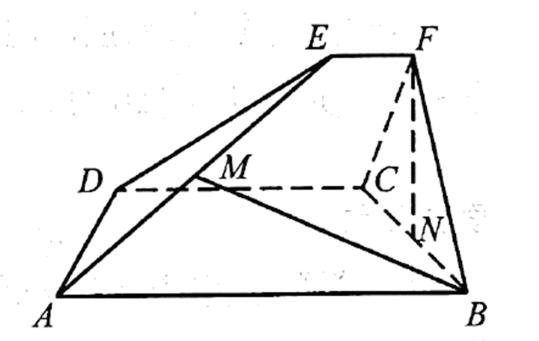
\includegraphics[width=.42\linewidth]{assets/asset-100-01.jpg}
\end{center}
\fillin[{$[12+2\sqrt{2}, 16]$}]
\begin{solution}
\textbf{答案：}$[12+2\sqrt{2}, 16]$

\textbf{分析：}根据正八边形的结构特征，分别以圆心为原点，$A_7A_3$ 所在直线为 $x$ 轴，$A_5A_1$ 所在直线为 $y$ 轴建立平面直角坐标系，即可求出各顶点的坐标，设 $P(x,y)$，再根据平面向量模的坐标计算公式即可得到 $\overrightarrow{PA_1}^2+\cdots+\overrightarrow{PA_8}^2 = 8(x^2+y^2)+8$，然后利用 $\cos 22.5^\circ \le |OP| \le 1$ 即可解出．

\textbf{详解：}建系如图，各顶点坐标：$A_1(0,1), A_2(\frac{\sqrt{2}}{2},\frac{\sqrt{2}}{2}), A_3(1,0), A_4(\frac{\sqrt{2}}{2},-\frac{\sqrt{2}}{2}), A_5(0,-1), A_6(-\frac{\sqrt{2}}{2},-\frac{\sqrt{2}}{2}), A_7(-1,0), A_8(-\frac{\sqrt{2}}{2},\frac{\sqrt{2}}{2})$．设 $P(x,y)$，则 $\sum PA_i^2 = 8(x^2+y^2)+8$．$|OP|$ 的最小值为 $\cos22.5^\circ = \frac{\sqrt{2+\sqrt{2}}}{2}$，最大值为1，所以 $x^2+y^2 \in [\frac{1+\cos45^\circ}{2},1] = [\frac{2+\sqrt{2}}{4},1]$，故取值范围为 $[12+2\sqrt{2},16]$.
\end{solution}
\end{question}

\begin{question}[points=14]
\textbf{来源：}2022 年 浙江卷，第 18 题\par
在 $\triangle ABC$ 中，角 $A,B,C$ 所对的边分别为 $a,b,c$．已知 $4a = \sqrt{5}c, \cos C = \frac{3}{5}$．

（1）求 $\sin A$ 的值；

（2）若 $b=11$，求 $\triangle ABC$ 的面积．
\begin{solution}
\textbf{答案：}（1）$\dfrac{\sqrt{5}}{5}$；（2）$22$

\textbf{分析：}（1）先由平方关系求出 $\sin C$，再根据正弦定理即可解出；（2）根据余弦定理以及 $4a=\sqrt{5}c$ 可解出 $a$，即可由三角形面积公式求出面积．

\textbf{详解：}（1）由 $\cos C = \frac{3}{5}$，$0<C<\pi$，得 $\sin C = \frac{4}{5}$．由 $4a=\sqrt{5}c$ 及正弦定理得 $4\sin A = \sqrt{5}\sin C$，所以 $\sin A = \frac{\sqrt{5}}{4}\cdot\frac{4}{5} = \frac{\sqrt{5}}{5}$．
（2）由 $4a=\sqrt{5}c$ 设 $c = \frac{4}{\sqrt{5}}a$，由余弦定理 $\cos C = \frac{a^2+b^2-c^2}{2ab} = \frac{a^2+121-\frac{16}{5}a^2}{2\cdot a\cdot11} = \frac{3}{5}$，解得 $a=5$（负值舍去），所以 $\triangle ABC$ 的面积 $S = \frac{1}{2}ab\sin C = \frac{1}{2}\times5\times11\times\frac{4}{5}=22$．
\end{solution}
\end{question}

\section*{2023 年}

\begin{question}[points=4]
\textbf{来源：}2023 年 北京卷，第 3 题\par
已知向量 $\vec{a}, \vec{b}$ 满足 $\vec{a} + \vec{b} = (2,3), \vec{a} - \vec{b} = (-2,1)$ ，则 $|\vec{a}|^2 - |\vec{b}|^2 =$ （ ）
\begin{choices}
  \item $-2$
  \item $-1$
  \item $0$
  \item $1$
\end{choices}
\begin{solution}
\textbf{答案：}B

\textbf{分析：}利用平面向量数量积的运算律，数量积的坐标表示求解作答.

\textbf{详解：}向量 $\vec{a}, \vec{b}$ 满足 $\vec{a} + \vec{b} = (2,3), \vec{a} - \vec{b} = (-2,1)$ ，所以 $|\vec{a}|^2 - |\vec{b}|^2 = (\vec{a}+\vec{b})\cdot(\vec{a}-\vec{b}) = 2\times(-2) + 3\times1 = -1$ .
\end{solution}
\end{question}

\begin{question}[points=4]
\textbf{来源：}2023 年 北京卷，第 7 题\par
在 $\triangle ABC$ 中， $(a+c)(\sin A - \sin C) = b(\sin A - \sin B)$ ，则 $\angle C =$ （ ）
\begin{choices}
  \item $\dfrac{\pi}{6}$
  \item $\dfrac{\pi}{3}$
  \item $\dfrac{2\pi}{3}$
  \item $\dfrac{5\pi}{6}$
\end{choices}
\begin{solution}
\textbf{答案：}B

\textbf{分析：}利用正弦定理的边角变换与余弦定理即可得解.

\textbf{详解：}因为 $(a+c)(\sin A - \sin C) = b(\sin A - \sin B)$，所以由正弦定理得 $(a+c)(a-c) = b(a-b)$，即 $a^2 - c^2 = ab - b^2$，则 $a^2 + b^2 - c^2 = ab$，故 $\cos C = \dfrac{a^2+b^2-c^2}{2ab} = \dfrac{ab}{2ab} = \dfrac{1}{2}$，又 $0 < C < \pi$，所以 $C = \dfrac{\pi}{3}$.
\end{solution}
\end{question}

\begin{question}[points=5]
\textbf{来源：}2023 年 全国甲卷-理科，第 4 题\par
已知向量 $\vec{a}$，$\vec{b}$，$\vec{c}$ 满足 $|\vec{a}| = |\vec{b}| = 1$，$|\vec{c}| = \sqrt{2}$，且 $\vec{a} + \vec{b} + \vec{c} = 0$，则 $\cos\langle \vec{a} - \vec{c}, \vec{b} - \vec{c} \rangle = $ （               ）
\begin{choices}
  \item $-\frac{4}{5}$
  \item $-\frac{2}{5}$
  \item $\frac{2}{5}$
  \item $\frac{4}{5}$
\end{choices}
\begin{solution}
\textbf{答案：}D

\textbf{分析：}作出图形，根据几何意义求解．

\textbf{详解：}因为 $\vec{a} + \vec{b} + \vec{c} = \vec{0}$，所以 $\vec{a} + \vec{b} = -\vec{c}$，即 $|\vec{a}|^2 + |\vec{b}|^2 + 2\vec{a} \cdot \vec{b} = |\vec{c}|^2$，即 $1 + 1 + 2\vec{a} \cdot \vec{b} = 2$，所以 $\vec{a} \cdot \vec{b} = 0$．如图，设 $\overrightarrow{OA} = \vec{a}$，$\overrightarrow{OB} = \vec{b}$，$\overrightarrow{OC} = \vec{c}$，由题知 $OA = OB = 1$，$OC = \sqrt{2}$，$\triangle OAB$ 是等腰直角三角形，$AB$ 边上的高 $OD = \frac{\sqrt{2}}{2}$，$AD = \frac{\sqrt{2}}{2}$，所以 $CD = CO + OD = \sqrt{2} + \frac{\sqrt{2}}{2} = \frac{3\sqrt{2}}{2}$，$\tan \angle ACD = \frac{AD}{CD} = \frac{1}{3}$，$\cos \angle ACD = \frac{3}{\sqrt{10}}$，$\cos\langle \vec{a} - \vec{c}, \vec{b} - \vec{c} \rangle = \cos \angle ACB = \cos 2\angle ACD = 2\cos^2 \angle ACD - 1 = 2 \times \frac{9}{10} - 1 = \frac{4}{5}$．
\end{solution}
\end{question}

\begin{question}[points=5]
\textbf{来源：}2023 年 全国甲卷-理科，第 16 题\par
在 $\triangle ABC$ 中，$\angle BAC = 60^\circ$，$AB = 2$，$BC = \sqrt{6}$，$\angle BAC$ 的角平分线交 $BC$ 于 $D$，则 $AD = $．
\fillin[{$2$}]
\begin{solution}
\textbf{答案：}$2$

\textbf{分析：}方法一：利用余弦定理求出 $AC$，再根据等面积法求出 $AD$；方法二：利用余弦定理求出 $AC$，再根据正弦定理求出 $B$，$C$，即可根据三角形的特征求出．

\textbf{详解：}方法一：记 $AB=c$，$AC=b$，$BC=a$，由余弦定理可得，$2^2+b^2-2\times2\times b\times\cos60^\circ = 6$，因为 $b>0$，解得：$b=1+\sqrt{3}$，由 $S_{\triangle ABC} = S_{\triangle ABD} + S_{\triangle ACD}$ 可得，$\frac{1}{2}\times2\times b\times\sin60^\circ = \frac{1}{2}\times2\times AD\times\sin30^\circ + \frac{1}{2}\times AD\times b\times\sin30^\circ$，解得：$AD = \frac{\sqrt{3}b}{1+\frac{b}{2}} = \frac{\sqrt{3}(1+\sqrt{3})}{\frac{3+\sqrt{3}}{2}} = 2$．故答案为：2．
方法二：由余弦定理可得，$2^2+b^2-2\times2\times b\times\cos60^\circ = 6$，因为 $b>0$，解得：$b=1+\sqrt{3}$，由正弦定理可得，$\frac{\sqrt{6}}{\sin60^\circ} = \frac{b}{\sin B} = \frac{2}{\sin C}$，解得：$\sin B = \frac{\sqrt{6}+\sqrt{2}}{4}$，$\sin C = \frac{\sqrt{2}}{2}$，因为 $1+\sqrt{3} > \sqrt{6} > 2$，所以 $C=45^\circ$，$B=180^\circ-60^\circ-45^\circ=75^\circ$，又 $\angle BAD = 30^\circ$，所以 $\angle ADB = 75^\circ$，即 $AD = AB = 2$．故答案为：2．
\end{solution}
\end{question}

\begin{question}[points=5]
\textbf{来源：}2023 年 全国甲卷-文科，第 3 题\par
已知向量 $\vec{a} = (3,1), \vec{b} = (2,2)$，则 $\cos\langle \vec{a}+\vec{b}, \vec{a}-\vec{b} \rangle =$（    ）
\begin{choices}
  \item $\frac{1}{17}$
  \item $\frac{\sqrt{17}}{17}$
  \item $\frac{\sqrt{5}}{5}$
  \item $\frac{2\sqrt{5}}{5}$
\end{choices}
\begin{solution}
\textbf{答案：}B

\textbf{分析：}利用平面向量模与数量积的坐标表示分别求得 $|\vec{a}+\vec{b}|, |\vec{a}-\vec{b}|, (\vec{a}+\vec{b})\cdot(\vec{a}-\vec{b})$，从而利用平面向量余弦的运算公式即可得解.

\textbf{详解：}因为 $\vec{a} = (3,1), \vec{b} = (2,2)$，所以 $\vec{a}+\vec{b} = (5,3), \vec{a}-\vec{b} = (1,-1)$，则 $|\vec{a}+\vec{b}| = \sqrt{5^2+3^2} = \sqrt{34}, |\vec{a}-\vec{b}| = \sqrt{1+1} = \sqrt{2}, (\vec{a}+\vec{b})\cdot(\vec{a}-\vec{b}) = 5\times1+3\times(-1)=2$，所以 $\cos\langle \vec{a}+\vec{b}, \vec{a}-\vec{b} \rangle = \frac{2}{\sqrt{34}\times\sqrt{2}} = \frac{\sqrt{17}}{17}$，故选B.
\end{solution}
\end{question}

\begin{question}
\textbf{来源：}2023 年 全国甲卷-文科，第 17 题\par
记 $\triangle ABC$ 的内角 $A,B,C$ 的对边分别为 $a,b,c$，已知 $\frac{b^2+c^2-a^2}{\cos A}=2$．

（1）求 $bc$；

（2）若 $\frac{a\cos B-b\cos A}{a\cos B+b\cos A}-\frac{b}{c}=1$，求 $\triangle ABC$ 面积．
\begin{solution}
\textbf{答案：}（1）$bc=1$；（2）$\frac{\sqrt{3}}{4}$

\textbf{分析：}（1）根据余弦定理即可解出；（2）由（1）可知，只需求出 $\sin A$ 即可得到三角形面积，对等式恒等变换，即可解出．

\textbf{详解：}（1）因为 $a^2=b^2+c^2-2bc\cos A$，所以 $\frac{b^2+c^2-a^2}{\cos A}=\frac{2bc\cos A}{\cos A}=2bc=2$，解得 $bc=1$．
（2）由正弦定理可得 $\frac{a\cos B-b\cos A}{a\cos B+b\cos A}-\frac{b}{c}=\frac{\sin A\cos B-\sin B\cos A}{\sin A\cos B+\sin B\cos A}-\frac{\sin B}{\sin C}=\frac{\sin(A-B)}{\sin(A+B)}-\frac{\sin B}{\sin(A+B)}=\frac{\sin(A-B)-\sin B}{\sin(A+B)}=1$，变形可得 $\sin(A-B)-\sin(A+B)=\sin B$，即 $-2\cos A\sin B=\sin B$，而 $0<\sin B\le1$，所以 $\cos A=-\frac{1}{2}$，又 $0<A<\pi$，所以 $\sin A=\frac{\sqrt{3}}{2}$，故 $\triangle ABC$ 的面积为 $S_{\triangle ABC}=\frac{1}{2}bc\sin A=\frac{1}{2}\times1\times\frac{\sqrt{3}}{2}=\frac{\sqrt{3}}{4}$．
\end{solution}
\end{question}

\begin{question}[points=5]
\textbf{来源：}2023 年 全国乙卷-理科，第 12 题\par
已知 $\odot O$ 的半径为1，直线 $PA$ 与 $\odot O$ 相切于点 $A$，直线 $PB$ 与 $\odot O$ 交于 $B$，$C$ 两点，$D$ 为 $BC$ 的中点，若 $PO=\sqrt{2}$，则 $\overrightarrow{PA}\cdot\overrightarrow{PD}$ 的最大值为（ ）
\begin{choices}
  \item $\frac{1+\sqrt{2}}{2}$
  \item $\frac{1+2\sqrt{2}}{2}$
  \item $1+\sqrt{2}$
  \item $2+\sqrt{2}$
\end{choices}
\begin{solution}
\textbf{答案：}$\frac{1+\sqrt{2}}{2}$

\textbf{分析：}由题意作出示意图，然后分类讨论，利用平面向量的数量积定义可得 $\overrightarrow{PA}\cdot\overrightarrow{PD}=\frac{1}{2}-\frac{\sqrt{2}}{2}\sin(2\alpha-\frac{\pi}{4})$，或 $\overrightarrow{PA}\cdot\overrightarrow{PD}=\frac{1}{2}+\frac{\sqrt{2}}{2}\sin(2\alpha+\frac{\pi}{4})$，然后结合三角函数的性质即可确定 $\overrightarrow{PA}\cdot\overrightarrow{PD}$ 的最大值.

\textbf{详解：}如图所示，$OA=1,OP=\sqrt{2}$，则由题意可知 $\angle APO=45^\circ$，由勾股定理可得 $PA=\sqrt{OP^2-OA^2}=1$. 当点 $A,D$ 位于直线 $PO$ 异侧时，设 $\angle OPC=\alpha$，$0\le\alpha\le \frac{\pi}{4}$，则 $\overrightarrow{PA}\cdot\overrightarrow{PD}=|PA|\cdot|PD|\cos(\alpha+\frac{\pi}{4})=1\times\sqrt{2}\cos\alpha\cos(\alpha+\frac{\pi}{4})=\sqrt{2}\cos\alpha(\frac{\sqrt{2}}{2}\cos\alpha-\frac{\sqrt{2}}{2}\sin\alpha)=\cos^2\alpha-\sin\alpha\cos\alpha=\frac{1+\cos2\alpha}{2}-\frac{1}{2}\sin2\alpha=\frac{1}{2}-\frac{\sqrt{2}}{2}\sin(2\alpha-\frac{\pi}{4})$，当 $2\alpha-\frac{\pi}{4}=-\frac{\pi}{4}$ 时，$\overrightarrow{PA}\cdot\overrightarrow{PD}$ 有最大值1. 当点 $A,D$ 位于直线 $PO$ 同侧时，设 $\angle OPC=\alpha$，$0\le\alpha\le \frac{\pi}{4}$，则 $\overrightarrow{PA}\cdot\overrightarrow{PD}=|PA|\cdot|PD|\cos(\alpha-\frac{\pi}{4})=1\times\sqrt{2}\cos\alpha\cos(\alpha-\frac{\pi}{4})=\sqrt{2}\cos\alpha(\frac{\sqrt{2}}{2}\cos\alpha+\frac{\sqrt{2}}{2}\sin\alpha)=\cos^2\alpha+\sin\alpha\cos\alpha=\frac{1+\cos2\alpha}{2}+\frac{1}{2}\sin2\alpha=\frac{1}{2}+\frac{\sqrt{2}}{2}\sin(2\alpha+\frac{\pi}{4})$，当 $2\alpha+\frac{\pi}{4}=\frac{\pi}{2}$ 时，$\overrightarrow{PA}\cdot\overrightarrow{PD}$ 有最大值 $\frac{1+\sqrt{2}}{2}$. 综上可得，$\overrightarrow{PA}\cdot\overrightarrow{PD}$ 的最大值为 $\frac{1+\sqrt{2}}{2}$.
\end{solution}
\end{question}

\begin{question}[points=12]
\textbf{来源：}2023 年 全国乙卷-理科，第 18 题\par
在 $\triangle ABC$ 中，已知 $\angle BAC=120^\circ$，$AB=2$，$AC=1$.



(1) 求 $\sin\angle ABC$；



(2) 若 $D$ 为 $BC$ 上一点，且 $\angle BAD=90^\circ$，求 $\triangle ADC$ 的面积.
\begin{solution}

\textbf{详解：}(1) 由余弦定理可得：$BC^2=AB^2+AC^2-2AB\cdot AC\cos A=4+1-2\times2\times1\times\cos120^\circ=7$，则 $BC=\sqrt{7}$，$\cos B=\frac{BC^2+AB^2-AC^2}{2BC\cdot AB}=\frac{7+4-1}{2\times2\times\sqrt{7}}=\frac{5\sqrt{7}}{14}$，$\sin B=\sqrt{1-\cos^2B}=\sqrt{1-\frac{25}{28}}=\frac{\sqrt{21}}{14}$.

(2) 由三角形面积公式可得 $\frac{S_{\triangle ABD}}{S_{\triangle ACD}}=\frac{\frac{1}{2}\times AB\times AD\times\sin90^\circ}{\frac{1}{2}\times AC\times AD\times\sin30^\circ}=4$，则 $S_{\triangle ACD}=\frac{1}{5}S_{\triangle ABC}=\frac{1}{5}\times\frac{1}{2}\times2\times1\times\sin120^\circ=\frac{3}{10}$.
\end{solution}
\end{question}

\begin{question}[points=5]
\textbf{来源：}2023 年 全国乙卷-文科，第 4 题\par
在$\triangle ABC$中，内角$A,B,C$的对边分别是$a,b,c$，若$a\cos B-b\cos A=c$，且$C=\frac{\pi}{5}$，则$\angle B=$（   ）
\begin{choices}
  \item $\frac{\pi}{10}$
  \item $\frac{\pi}{5}$
  \item $\frac{3\pi}{10}$
  \item $\frac{2\pi}{5}$
\end{choices}
\begin{solution}
\textbf{答案：}$\frac{3\pi}{10}$

\textbf{分析：}首先利用正弦定理边化角，然后结合诱导公式和两角和的正弦公式求得$\angle A$的值，最后利用三角形内角和定理可得$\angle B$的值.

\textbf{详解：}由题意结合正弦定理得$\sin A\cos B-\sin B\cos A=\sin C$，即$\sin A\cos B-\sin B\cos A=\sin(A+B)=\sin A\cos B+\sin B\cos A$，整理得$\sin B\cos A=0$，由于$B\in(0,\pi)$，故$\sin B>0$，据此可得$\cos A=0$，$A=\frac{\pi}{2}$，则$B=\pi-A-C=\pi-\frac{\pi}{2}-\frac{\pi}{5}=\frac{3\pi}{10}$. 故选C.
\end{solution}
\end{question}

\begin{question}[points=5]
\textbf{来源：}2023 年 全国乙卷-文科，第 6 题\par
正方形$ABCD$的边长是2，$E$是$AB$的中点，则$\overrightarrow{EC}\cdot\overrightarrow{ED}=$（   ）

\begin{center}
  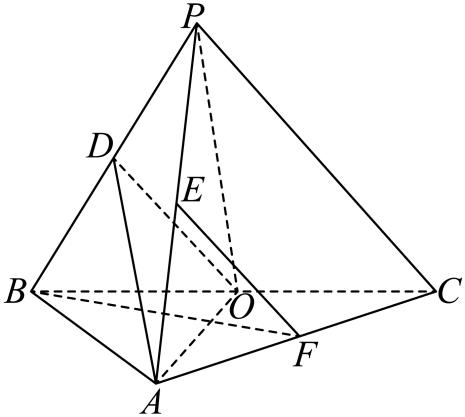
\includegraphics[width=.42\linewidth]{assets/asset-111-01.jpg}
\end{center}
\begin{choices}
  \item $\sqrt{5}$
  \item $3$
  \item $2\sqrt{5}$
  \item $5$
\end{choices}
\begin{solution}
\textbf{答案：}$3$

\textbf{分析：}方法一：以$\overrightarrow{AB},\overrightarrow{AD}$为基底向量表示$\overrightarrow{EC},\overrightarrow{ED}$，再结合数量积的运算律运算求解；方法二：建系，利用平面向量的坐标运算求解；方法三：利用余弦定理求$\cos\angle DEC$，进而根据数量积的定义运算求解.

\textbf{详解：}方法一：以$\overrightarrow{AB},\overrightarrow{AD}$为基底向量，可知$|\overrightarrow{AB}|=|\overrightarrow{AD}|=2$，$\overrightarrow{AB}\cdot\overrightarrow{AD}=0$，则$\overrightarrow{EC}=\overrightarrow{EB}+\overrightarrow{BC}=\frac{1}{2}\overrightarrow{AB}+\overrightarrow{AD}$，$\overrightarrow{ED}=\overrightarrow{EA}+\overrightarrow{AD}=-\frac{1}{2}\overrightarrow{AB}+\overrightarrow{AD}$，所以$\overrightarrow{EC}\cdot\overrightarrow{ED}=(\frac{1}{2}\overrightarrow{AB}+\overrightarrow{AD})\cdot(-\frac{1}{2}\overrightarrow{AB}+\overrightarrow{AD})=-\frac{1}{4}|\overrightarrow{AB}|^2+|\overrightarrow{AD}|^2=-1+4=3$；
方法二：如图，以$A$为坐标原点建立平面直角坐标系，则$E(1,0), C(2,2), D(0,2)$，可得$\overrightarrow{EC}=(1,2), \overrightarrow{ED}=(-1,2)$，所以$\overrightarrow{EC}\cdot\overrightarrow{ED}=-1+4=3$；
方法三：由题意可得$ED=EC=\sqrt{5}, CD=2$，在$\triangle CDE$中，由余弦定理得$\cos\angle DEC=\frac{DE^2+CE^2-DC^2}{2\cdot DE\cdot CE}=\frac{5+5-4}{2\times\sqrt{5}\times\sqrt{5}}=\frac{3}{5}$，所以$\overrightarrow{EC}\cdot\overrightarrow{ED}=|\overrightarrow{EC}||\overrightarrow{ED}|\cos\angle DEC=\sqrt{5}\times\sqrt{5}\times\frac{3}{5}=3$. 故选B.
\end{solution}
\end{question}

\begin{question}[points=5]
\textbf{来源：}2023 年 上海卷，第 7 题\par
已知 $\triangle ABC$ 的面积为 $\sqrt{3}$，$AB=2$，$AC=3$，求 $\angle A=$
\fillin[{$\frac{\pi}{3}$ 或 $\frac{2\pi}{3}$}]
\begin{solution}
\textbf{答案：}$\frac{\pi}{3}$ 或 $\frac{2\pi}{3}$
\end{solution}
\end{question}

\begin{question}[points=5]
\textbf{来源：}2023 年 上海卷，第 8 题\par
在 $\triangle ABC$ 中，$a=2$，$b=3$，$\cos C = \frac{1}{4}$，求 $c=$
\fillin[{$\sqrt{10}$}]
\begin{solution}
\textbf{答案：}$\sqrt{10}$
\end{solution}
\end{question}

\begin{question}[points=5]
\textbf{来源：}2023 年 天津卷，第 14 题\par
在 $\triangle ABC$ 中，$\angle A = 60^\circ$，$BC = 1$，点 $D$ 为 $AB$ 的中点，点 $E$ 为 $CD$ 的中点，若设 $\overrightarrow{AB} = \vec{a}$，$\overrightarrow{AC} = \vec{b}$，则 $\overrightarrow{AE}$ 可用 $\vec{a}, \vec{b}$ 表示为；若 $\overrightarrow{BF} = \dfrac{1}{3} \overrightarrow{BC}$，则 $\overrightarrow{AE} \cdot \overrightarrow{AF}$ 的最大值为．
\fillin[{$\dfrac{1}{4}\vec{a} + \dfrac{1}{2}\vec{b}$ ; $\dfrac{13}{24}$}]
\begin{solution}
\textbf{答案：}$\dfrac{1}{4}\vec{a} + \dfrac{1}{2}\vec{b}$ ; $\dfrac{13}{24}$

\textbf{分析：}利用向量线性运算和数量积，结合余弦定理和基本不等式.

\textbf{详解：}因为 $E$ 为 $CD$ 的中点，则 $\overrightarrow{ED} + \overrightarrow{EC} = \vec{0}$，由 $\begin{cases} \overrightarrow{AE} + \overrightarrow{ED} = \overrightarrow{AD} \\ \overrightarrow{AE} + \overrightarrow{EC} = \overrightarrow{AC} \end{cases}$ 两式相加得 $2\overrightarrow{AE} = \overrightarrow{AD} + \overrightarrow{AC} = \dfrac{1}{2}\overrightarrow{AB} + \overrightarrow{AC} = \dfrac{1}{2}\vec{a} + \vec{b}$，所以 $\overrightarrow{AE} = \dfrac{1}{4}\vec{a} + \dfrac{1}{2}\vec{b}$. 因为 $\overrightarrow{BF} = \dfrac{1}{3}\overrightarrow{BC}$，则 $2\overrightarrow{FB} + \overrightarrow{FC} = \vec{0}$，由 $\begin{cases} \overrightarrow{AF} + \overrightarrow{FC} = \overrightarrow{AC} \\ \overrightarrow{AF} + \overrightarrow{FB} = \overrightarrow{AB} \end{cases}$ 两式相加得 $3\overrightarrow{AF} = 2\overrightarrow{AB} + \overrightarrow{AC} = 2\vec{a} + \vec{b}$，所以 $\overrightarrow{AF} = \dfrac{2}{3}\vec{a} + \dfrac{1}{3}\vec{b}$. 所以 $\overrightarrow{AE} \cdot \overrightarrow{AF} = \left(\dfrac{1}{4}\vec{a} + \dfrac{1}{2}\vec{b}\right) \cdot \left(\dfrac{2}{3}\vec{a} + \dfrac{1}{3}\vec{b}\right) = \dfrac{1}{12}(2|\vec{a}|^2 + 5\vec{a}\cdot\vec{b} + 2|\vec{b}|^2)$. 设 $AB = x$, $AC = y$, 则 $\vec{a}\cdot\vec{b} = xy\cos60^\circ = \dfrac{xy}{2}$, 且 $BC^2 = x^2 + y^2 - xy = 1$, 所以 $2x^2 + 5\cdot\frac{xy}{2} + 2y^2 = 2(x^2 + y^2) + \frac{5}{2}xy = 2(1+xy) + \frac{5}{2}xy = 2 + \frac{9}{2}xy$. 由 $x^2 + y^2 \ge 2xy$ 得 $1 = x^2 + y^2 - xy \ge xy$, 即 $xy \le 1$, 当 $x = y = 1$ 时取等. 所以 $\overrightarrow{AE} \cdot \overrightarrow{AF} = \dfrac{1}{12}\left(2 + \frac{9}{2}xy\right) \le \dfrac{1}{12}\left(2 + \frac{9}{2}\right) = \dfrac{13}{24}$.
\end{solution}
\end{question}

\begin{question}[points=14]
\textbf{来源：}2023 年 天津卷，第 16 题\par
在 $\triangle ABC$ 中，角 $A, B, C$ 所对的边分别是 $a, b, c$．已知 $a = \sqrt{39}$, $b = 2$, $\angle A = 120^\circ$．

(1) 求 $\sin B$ 的值；

(2) 求 $c$ 的值；

(3) 求 $\sin(B - C)$．
\begin{solution}
\textbf{答案：}(1) $\dfrac{\sqrt{13}}{13}$ ; (2) $5$ ; (3) $-\dfrac{7\sqrt{3}}{26}$

\textbf{详解：}(1) 由正弦定理 $\dfrac{a}{\sin A} = \dfrac{b}{\sin B}$, 得 $\dfrac{\sqrt{39}}{\sin120^\circ} = \dfrac{2}{\sin B}$, 解得 $\sin B = \dfrac{\sqrt{13}}{13}$.
(2) 由余弦定理 $a^2 = b^2 + c^2 - 2bc\cos A$, 即 $39 = 4 + c^2 - 2\cdot 2 \cdot c \cdot \left(-\frac{1}{2}\right) = 4 + c^2 + 2c$, 整理得 $c^2 + 2c - 35 = 0$, 解得 $c = 5$ (负值舍去).
(3) 由正弦定理 $\dfrac{a}{\sin A} = \dfrac{c}{\sin C}$ 得 $\dfrac{\sqrt{39}}{\sin120^\circ} = \dfrac{5}{\sin C}$, 解得 $\sin C = \dfrac{5\sqrt{13}}{26}$. 因为 $A = 120^\circ$, 所以 $B, C$ 均为锐角, $\cos B = \sqrt{1-\left(\frac{\sqrt{13}}{13}\right)^2} = \dfrac{2\sqrt{39}}{13}$, $\cos C = \sqrt{1-\left(\frac{5\sqrt{13}}{26}\right)^2} = \dfrac{\sqrt{39}}{26}$. 所以 $\sin(B-C) = \sin B \cos C - \cos B \sin C = \dfrac{\sqrt{13}}{13} \cdot \dfrac{\sqrt{39}}{26} - \dfrac{2\sqrt{39}}{13} \cdot \dfrac{5\sqrt{13}}{26} = -\dfrac{7\sqrt{3}}{26}$.
\end{solution}
\end{question}

\begin{question}[points=5]
\textbf{来源：}2023 年 新高考II卷，第 13 题\par
已知向量$\vec{a}$，$\vec{b}$满足$|\vec{a}-\vec{b}|=\sqrt{3}$，$|\vec{a}+\vec{b}|=|2\vec{a}-\vec{b}|$，则$|\vec{b}|=$ ．
\fillin[{$\sqrt{3}$}]
\begin{solution}
\textbf{答案：}$\sqrt{3}$

\textbf{分析：}法一：根据题意结合向量数量积的运算律运算求解；法二：换元令$\vec{c}=\vec{a}-\vec{b}$，结合数量积的运算律运算求解.

\textbf{详解：}法一：因为$|\vec{a}+\vec{b}|=|2\vec{a}-\vec{b}|$，即$(\vec{a}+\vec{b})^{2}=(2\vec{a}-\vec{b})^{2}$，则$\vec{a}^{2}+2\vec{a}\cdot\vec{b}+\vec{b}^{2}=4\vec{a}^{2}-4\vec{a}\cdot\vec{b}+\vec{b}^{2}$，整理得$\vec{a}^{2}-2\vec{a}\cdot\vec{b}=0$，又因为$|\vec{a}-\vec{b}|=\sqrt{3}$，即$(\vec{a}-\vec{b})^{2}=3$，则$\vec{a}^{2}-2\vec{a}\cdot\vec{b}+\vec{b}^{2}=|\vec{b}|^{2}=3$，所以$|\vec{b}|=\sqrt{3}$.
法二：设$\vec{c}=\vec{a}-\vec{b}$，则$|\vec{c}|=\sqrt{3}$，$\vec{a}+\vec{b}=\vec{c}+2\vec{b}$，$2\vec{a}-\vec{b}=2\vec{c}+\vec{b}$，由题意可得$(\vec{c}+2\vec{b})^{2}=(2\vec{c}+\vec{b})^{2}$，则$\vec{c}^{2}+4\vec{c}\cdot\vec{b}+4\vec{b}^{2}=4\vec{c}^{2}+4\vec{c}\cdot\vec{b}+\vec{b}^{2}$，整理得$\vec{c}^{2}=\vec{b}^{2}$，即$|\vec{b}|=|\vec{c}|=\sqrt{3}$.
\end{solution}
\end{question}

\begin{question}[points=10]
\textbf{来源：}2023 年 新高考II卷，第 17 题\par
记$\triangle ABC$的内角$A,B,C$的对边分别为$a,b,c$，已知$\triangle ABC$的面积为$\sqrt{3}$，$D$为$BC$中点，且$AD=1$．

（1）若$\angle ADC=\dfrac{\pi}{3}$，求$\tan B$；

（2）若$b^{2}+c^{2}=8$，求$b,c$．
\begin{solution}
\textbf{答案：}（1）$\dfrac{\sqrt{3}}{5}$；（2）$b=c=2$.

\textbf{分析：}（1）方法1，利用三角形面积公式求出$a$，再利用余弦定理求解作答；方法2，利用三角形面积公式求出$a$，作出$BC$边上的高，利用直角三角形求解作答.
（2）方法1，利用余弦定理求出$a$，再利用三角形面积公式求出$\angle ADC$即可求解作答；方法2，利用向量运算律建立关系求出$a$，再利用三角形面积公式求出$\angle ADC$即可求解作答.

\textbf{详解：}（1）方法1：在$\triangle ABC$中，因为$D$为$BC$中点，$\angle ADC=\dfrac{\pi}{3}$，$AD=1$，则$S_{\triangle ADC}=\dfrac{1}{2}AD\cdot DC\sin\angle ADC=\dfrac{1}{2}\times1\times\dfrac{a}{2}\times\dfrac{\sqrt{3}}{2}=\dfrac{\sqrt{3}}{8}a=\dfrac{1}{2}S_{\triangle ABC}=\dfrac{\sqrt{3}}{2}$，解得$a=4$，在$\triangle ABD$中，$\angle ADB=\dfrac{2\pi}{3}$，由余弦定理得$c^{2}=BD^{2}+AD^{2}-2BD\cdot AD\cos\angle ADB$，即$c^{2}=4+1-2\times2\times1\times(-\dfrac{1}{2})=7$，解得$c=\sqrt{7}$，则$\cos B=\dfrac{7+4-1}{2\times\sqrt{7}\times2}=\dfrac{5\sqrt{7}}{14}$，$\sin B=\sqrt{1-\cos^{2}B}=\sqrt{1-\left(\dfrac{5\sqrt{7}}{14}\right)^{2}}=\dfrac{\sqrt{21}}{14}$，所以$\tan B=\dfrac{\sin B}{\cos B}=\dfrac{\sqrt{3}}{5}$.
方法2：在$\triangle ABC$中，因为$D$为$BC$中点，$\angle ADC=\dfrac{\pi}{3}$，$AD=1$，则$S_{\triangle ADC}=\dfrac{1}{2}AD\cdot DC\sin\angle ADC=\dfrac{1}{2}\times1\times\dfrac{a}{2}\times\dfrac{\sqrt{3}}{2}=\dfrac{\sqrt{3}}{8}a=\dfrac{1}{2}S_{\triangle ABC}=\dfrac{\sqrt{3}}{2}$，解得$a=4$，在$\triangle ACD$中，由余弦定理得$b^{2}=CD^{2}+AD^{2}-2CD\cdot AD\cos\angle ADC$，即$b^{2}=4+1-2\times2\times1\times\dfrac{1}{2}=3$，解得$b=\sqrt{3}$，有$AC^{2}+AD^{2}=4=CD^{2}$，则$\angle CAD=\dfrac{\pi}{2}$，$\angle C=\dfrac{\pi}{6}$，过$A$作$AE\perp BC$于$E$，于是$CE=AC\cos C=\dfrac{3}{2}$，$AE=AC\sin C=\dfrac{\sqrt{3}}{2}$，$BE=\dfrac{5}{2}$，所以$\tan B=\dfrac{AE}{BE}=\dfrac{\sqrt{3}}{5}$.
（2）方法1：在$\triangle ABD$与$\triangle ACD$中，由余弦定理得$\begin{cases}c^{2}=\dfrac{1}{4}a^{2}+1-2\times\dfrac{a}{2}\times1\times\cos(\pi-\angle ADC)\\ b^{2}=\dfrac{1}{4}a^{2}+1-2\times\dfrac{a}{2}\times1\times\cos\angle ADC\end{cases}$，整理得$\dfrac{1}{2}a^{2}+2=b^{2}+c^{2}$，而$b^{2}+c^{2}=8$，则$a=2\sqrt{3}$，又$S_{\triangle ADC}=\dfrac{1}{2}\times\sqrt{3}\times1\times\sin\angle ADC=\dfrac{\sqrt{3}}{2}$，解得$\sin\angle ADC=1$，而$0<\angle ADC<\pi$，于是$\angle ADC=\dfrac{\pi}{2}$，所以$b=c=\sqrt{AD^{2}+CD^{2}}=2$.
方法2：在$\triangle ABC$中，因为$D$为$BC$中点，则$2\overrightarrow{AD}=\overrightarrow{AB}+\overrightarrow{AC}$，又$\overrightarrow{CB}=\overrightarrow{AB}-\overrightarrow{AC}$，于是$4|\overrightarrow{AD}|^{2}+|\overrightarrow{CB}|^{2}=(\overrightarrow{AB}+\overrightarrow{AC})^{2}+(\overrightarrow{AB}-\overrightarrow{AC})^{2}=2(b^{2}+c^{2})=16$，即$4+a^{2}=16$，解得$a=2\sqrt{3}$，又$S_{\triangle ADC}=\dfrac{1}{2}\times\sqrt{3}\times1\times\sin\angle ADC=\dfrac{\sqrt{3}}{2}$，解得$\sin\angle ADC=1$，而$0<\angle ADC<\pi$，于是$\angle ADC=\dfrac{\pi}{2}$，所以$b=c=\sqrt{AD^{2}+CD^{2}}=2$.
\end{solution}
\end{question}

\begin{question}[points=5]
\textbf{来源：}2023 年 新高考I卷，第 3 题\par
已知向量 $\vec{a}=(1,1),\vec{b}=(1,-1)$，若 $(\vec{a}+\lambda\vec{b})\perp(\vec{a}+\mu\vec{b})$，则（ ）
\begin{choices}
  \item $\lambda+\mu=1$
  \item $\lambda+\mu=-1$
  \item $\lambda\mu=1$
  \item $\lambda\mu=-1$
\end{choices}
\begin{solution}
\textbf{答案：}$\lambda\mu=-1$

\textbf{分析：}根据向量的坐标运算求出 $\vec{a}+\lambda\vec{b}$，$\vec{a}+\mu\vec{b}$，再根据向量垂直的坐标表示即可求出。

\textbf{详解：}因为 $\vec{a}=(1,1),\vec{b}=(1,-1)$，所以 $\vec{a}+\lambda\vec{b}=(1+\lambda,1-\lambda)$，$\vec{a}+\mu\vec{b}=(1+\mu,1-\mu)$，由 $(\vec{a}+\lambda\vec{b})\perp(\vec{a}+\mu\vec{b})$ 可得 $(\vec{a}+\lambda\vec{b})\cdot(\vec{a}+\mu\vec{b})=0$，即 $(1+\lambda)(1+\mu)+(1-\lambda)(1-\mu)=0$，整理得：$\lambda\mu=-1$。
\end{solution}
\end{question}

\begin{question}[points=10]
\textbf{来源：}2023 年 新高考I卷，第 17 题\par
已知在 $\triangle ABC$ 中，$A+B=3C, 2\sin(A-C)=\sin B$．

（1）求 $\sin A$；

（2）设 $AB=5$，求 $AB$ 边上的高．
\begin{solution}
\textbf{答案：}（1）$\frac{3\sqrt{10}}{10}$；（2）6

\textbf{分析：}（1）根据角的关系及两角和差正弦公式，化简即可得解；（2）利用同角之间的三角函数基本关系及两角和的正弦公式求 $\sin B$，再由正弦定理求出 $b$，根据等面积法求解即可。

\textbf{详解：}（1）因为 $A+B=3C$，所以 $\pi-C=3C$，即 $C=\frac{\pi}{4}$，又 $2\sin(A-C)=\sin B=\sin(A+C)$，所以 $2\sin A\cos C-2\cos A\sin C=\sin A\cos C+\cos A\sin C$，所以 $\sin A\cos C=3\cos A\sin C$，所以 $\sin A=3\cos A$，即 $\tan A=3$，所以 $0<A<\frac{\pi}{2}$，所以 $\sin A=\frac{3}{\sqrt{10}}=\frac{3\sqrt{10}}{10}$。（2）由（1）知，$\cos A=\frac{1}{\sqrt{10}}=\frac{\sqrt{10}}{10}$，由 $\sin B=\sin(A+C)=\sin A\cos C+\cos A\sin C=\frac{\sqrt{2}}{2}(\frac{3\sqrt{10}}{10}+\frac{\sqrt{10}}{10})=\frac{2\sqrt{5}}{5}$，由正弦定理 $\frac{c}{\sin C}=\frac{b}{\sin B}$，可得 $b=\frac{5\times\frac{2\sqrt{5}}{5}}{\frac{\sqrt{2}}{2}}=2\sqrt{10}$，因为 $\frac{1}{2}AB\cdot h=\frac{1}{2}AB\cdot AC\cdot\sin A$，所以 $h=b\cdot\sin A=2\sqrt{10}\times\frac{3\sqrt{10}}{10}=6$。
\end{solution}
\end{question}

\section*{2024 年}

\begin{question}[points=13]
\textbf{来源：}2024 年 北京卷，第 16 题\par
在 $\triangle ABC$ 中，$a=7$，$A$ 为钝角，$\sin 2B = \dfrac{\sqrt{3}}{7} b \cos B$。

（1）求 $\angle A$；

（2）从条件①、条件②和条件③这三个条件中选择一个作为已知，求 $\triangle ABC$ 的面积。

① $b=7$；② $\cos B = \dfrac{13}{14}$；③ $c\sin A = \dfrac{5}{2}\sqrt{3}$。

注：如果选择条件①、条件②和条件③分别解答，按第一个解答计分。
\begin{solution}
\textbf{答案：}（1）$A=\dfrac{2\pi}{3}$；（2）选择①无解；选择②和③ $\triangle ABC$ 面积均为 $\dfrac{15\sqrt{3}}{4}$。

\textbf{分析：}（1）利用正弦定理即可求出答案；（2）选择①，利用正弦定理得 $B=\dfrac{\pi}{3}$，结合（1）问答案即可排除；选择②，首先求出 $\sin B = \dfrac{3\sqrt{3}}{14}$，再代入式子得 $b=3$，再利用两角和的正弦公式即可求出 $\sin C$，最后利用三角形面积公式即可；选择③，首先得到 $c=5$，再利用正弦定理得到 $\sin C = \dfrac{5\sqrt{3}}{14}$，再利用两角和的正弦公式即可求出 $\sin B$，最后利用三角形面积公式即可。

\textbf{详解：}（1）由题意得 $2\sin B \cos B = \dfrac{\sqrt{3}}{7} b \cos B$，因为 $A$ 为钝角，则 $\cos B \neq 0$，则 $2\sin B = \dfrac{\sqrt{3}}{7} b$，则 $\sin B = \dfrac{\sqrt{3}}{14} b$，由正弦定理 $\dfrac{b}{\sin B} = \dfrac{a}{\sin A}$ 得 $\dfrac{b}{\frac{\sqrt{3}}{14}b} = \dfrac{7}{\sin A}$，解得 $\sin A = \dfrac{\sqrt{3}}{2}$，因为 $A$ 为钝角，则 $A = \dfrac{2\pi}{3}$。
（2）选择① $b=7$，则 $\sin B = \dfrac{\sqrt{3}}{14} \times 7 = \dfrac{\sqrt{3}}{2}$，因为 $A=\dfrac{2\pi}{3}$，则 $B$ 为锐角，则 $B = \dfrac{\pi}{3}$，此时 $A+B = \pi$，不合题意，舍弃。
选择② $\cos B = \dfrac{13}{14}$，因为 $B$ 为三角形内角，则 $\sin B = \sqrt{1-\left(\dfrac{13}{14}\right)^2} = \dfrac{3\sqrt{3}}{14}$，则代入 $2\sin B = \dfrac{\sqrt{3}}{7} b$ 得 $2\times \dfrac{3\sqrt{3}}{14} = \dfrac{\sqrt{3}}{7} b$，解得 $b=3$。$\sin C = \sin(A+B) = \sin\left(\dfrac{2\pi}{3}+B\right) = \sin\dfrac{2\pi}{3}\cos B + \cos\dfrac{2\pi}{3}\sin B = \dfrac{\sqrt{3}}{2}\times\dfrac{13}{14} + \left(-\dfrac{1}{2}\right)\times\dfrac{3\sqrt{3}}{14} = \dfrac{5\sqrt{3}}{14}$。则 $S_{\triangle ABC} = \dfrac{1}{2}ab\sin C = \dfrac{1}{2}\times7\times3\times\dfrac{5\sqrt{3}}{14} = \dfrac{15\sqrt{3}}{4}$。
选择③ $c\sin A = \dfrac{5}{2}\sqrt{3}$，则有 $c\times\dfrac{\sqrt{3}}{2} = \dfrac{5}{2}\sqrt{3}$，解得 $c=5$。则由正弦定理得 $\dfrac{a}{\sin A} = \dfrac{c}{\sin C}$，即 $\dfrac{7}{\frac{\sqrt{3}}{2}} = \dfrac{5}{\sin C}$，解得 $\sin C = \dfrac{5\sqrt{3}}{14}$。因为 $C$ 为三角形内角，则 $\cos C = \sqrt{1-\left(\dfrac{5\sqrt{3}}{14}\right)^2} = \dfrac{11}{14}$。则 $\sin B = \sin(A+C) = \sin\left(\dfrac{2\pi}{3}+C\right) = \sin\dfrac{2\pi}{3}\cos C + \cos\dfrac{2\pi}{3}\sin C = \dfrac{\sqrt{3}}{2}\times\dfrac{11}{14} + \left(-\dfrac{1}{2}\right)\times\dfrac{5\sqrt{3}}{14} = \dfrac{3\sqrt{3}}{14}$。则 $S_{\triangle ABC} = \dfrac{1}{2}ac\sin B = \dfrac{1}{2}\times7\times5\times\dfrac{3\sqrt{3}}{14} = \dfrac{15\sqrt{3}}{4}$。
\end{solution}
\end{question}

\begin{question}[points=5]
\textbf{来源：}2024 年 全国甲卷-理科，第 9 题；次专题：集合与逻辑\par
已知向量 $\vec{a}=(x+1,x),\vec{b}=(x,2)$，则（   ）
\begin{choices}
  \item “$x=-3$”是“$\vec{a}\perp\vec{b}$”的必要条件
  \item “$x=-3$”是“$\vec{a}\parallel\vec{b}$”的必要条件
  \item “$x=0$”是“$\vec{a}\perp\vec{b}$”的充分条件
  \item “$x=-1+\sqrt{3}$”是“$\vec{a}\parallel\vec{b}$”的充分条件
\end{choices}
\begin{solution}
\textbf{答案：}C

\textbf{分析：}根据向量垂直和平行的坐标表示即可得到方程，解出即可。

\textbf{详解：}对 A，当 $\vec{a}\perp\vec{b}$ 时，则 $\vec{a}\cdot\vec{b}=0$，所以 $x\cdot(x+1)+2x=0$，解得 $x=0$ 或 $-3$，即必要性不成立，故 A 错误；对 C，当 $x=0$ 时，$\vec{a}=(1,0),\vec{b}=(0,2)$，故 $\vec{a}\cdot\vec{b}=0$，所以 $\vec{a}\perp\vec{b}$，即充分性成立，故 C 正确；对 B，当 $\vec{a}\parallel\vec{b}$ 时，则 $2(x+1)=x^2$，解得 $x=1\pm\sqrt{3}$，即必要性不成立，故 B 错误；对 D，当 $x=-1+\sqrt{3}$ 时，不满足 $2(x+1)=x^2$，所以 $\vec{a}\parallel\vec{b}$ 不成立，即充分性不立，故 D 错误。
\end{solution}
\end{question}

\begin{question}[points=5]
\textbf{来源：}2024 年 全国甲卷-理科，第 11 题\par
在 $\triangle ABC$ 中内角 $A,B,C$ 所对边分别为 $a,b,c$，若 $B=\dfrac{\pi}{3}$，$b^2=\dfrac{9}{4}ac$，则 $\sin A+\sin C=$ （   ）
\begin{choices}
  \item $\dfrac{3}{2}$
  \item $\sqrt{2}$
  \item $\dfrac{\sqrt{7}}{2}$
  \item $\dfrac{3}{\sqrt{2}}$
\end{choices}
\begin{solution}
\textbf{答案：}C

\textbf{分析：}利用正弦定理得 $\sin A\sin C=\frac{1}{3}$，再利用余弦定理有 $a^2+c^2=\frac{13}{4}ac$，再利用正弦定理得到 $\sin^2 A+\sin^2 C$ 的值，最后代入计算即可。

\textbf{详解：}因为 $B=\frac{\pi}{3},b^2=\frac{9}{4}ac$，则由正弦定理得 $\sin A\sin C=\frac{4}{9}\sin^2 B=\frac{1}{3}$。由余弦定理可得 $b^2=a^2+c^2-ac=\frac{9}{4}ac$，即 $a^2+c^2=\frac{13}{4}ac$，根据正弦定理得 $\sin^2 A+\sin^2 C=\frac{13}{4}\sin A\sin C=\frac{13}{12}$，所以 $(\sin A+\sin C)^2=\sin^2 A+\sin^2 C+2\sin A\sin C=\frac{7}{4}$，因为 $A,C$ 为三角形内角，则 $\sin A+\sin C>0$，则 $\sin A+\sin C=\frac{\sqrt{7}}{2}$。
\end{solution}
\end{question}

\begin{question}[points=5]
\textbf{来源：}2024 年 全国甲卷-文科，第 11 题\par
在 $\triangle ABC$ 中，内角 $A, B, C$ 所对边分别为 $a, b, c$，若 $B = \frac{\pi}{3}$，$b^2 = \frac{9}{4}ac$，则 $\sin A + \sin C =$（ ）
\begin{choices}
  \item $\frac{3}{2}$
  \item $\sqrt{2}$
  \item $\frac{\sqrt{7}}{2}$
  \item $\frac{3}{2}$
\end{choices}
\begin{solution}
\textbf{答案：}C

\textbf{分析：}利用正弦定理得 $\sin A \sin C = \frac{1}{3}$，再利用余弦定理有 $a^2 + c^2 = \frac{13}{4}ac$，再利用正弦定理得到 $\sin^2 A + \sin^2 C$ 的值，最后代入计算即可.

\textbf{详解：}因为 $B = \frac{\pi}{3}$，$b^2 = \frac{9}{4}ac$，则由正弦定理得 $\sin A \sin C = \sin^2 B \cdot \frac{4}{9} = \left(\frac{\sqrt{3}}{2}\right)^2 \cdot \frac{4}{9} = \frac{1}{3}$．由余弦定理可得：$b^2 = a^2 + c^2 - ac = \frac{9}{4}ac$，即 $a^2 + c^2 = \frac{13}{4}ac$，根据正弦定理得 $\sin^2 A + \sin^2 C = \frac{13}{4} \sin A \sin C = \frac{13}{4} \times \frac{1}{3} = \frac{13}{12}$，所以 $(\sin A + \sin C)^2 = \sin^2 A + \sin^2 C + 2\sin A \sin C = \frac{13}{12} + \frac{2}{3} = \frac{21}{12} = \frac{7}{4}$，因为 $A, C$ 为三角形内角，则 $\sin A + \sin C > 0$，则 $\sin A + \sin C = \frac{\sqrt{7}}{2}$.
\end{solution}
\end{question}

\begin{question}[points=4]
\textbf{来源：}2024 年 上海卷，第 5 题\par
已知$k\in\mathbb{R}$，$\vec{a}=(2,5)$，$\vec{b}=(6,k)$，且$\vec{a}\parallel\vec{b}$，则$k$的值为.
\fillin[{$15$}]
\begin{solution}
\textbf{答案：}$15$

\textbf{分析：}根据向量平行的坐标表示得到方程，解出即可.

\textbf{详解：}$\because\vec{a}\parallel\vec{b}$，$\therefore 2k=5\times6$，解得$k=15$．故答案为：15.
\end{solution}
\end{question}

\begin{question}[points=5]
\textbf{来源：}2024 年 上海卷，第 11 题\par
已知点$B$在点$C$正北方向，点$D$在点$C$的正东方向，$BC=CD$，存在点$A$满足$\angle BAC=16.5^\circ$，$\angle DAC=37^\circ$，则$\angle BCA=$(精确到0.1度).
\fillin[{$7.8^\circ$}]
\begin{solution}
\textbf{答案：}$7.8^\circ$

\textbf{分析：}设$\angle BCA=\theta$，在$\triangle DCA$和$\triangle BCA$中分别利用正弦定理得到$\frac{CA}{\sin D}=\frac{CD}{\sin\angle CAD}$，$\frac{CA}{\sin(\theta+16.5^\circ)}=\frac{CB}{\sin16.5^\circ}$，两式相除即可得到答案.

\textbf{详解：}设$\angle BCA=\theta$，$\angle ACD=90^\circ-\theta$，在$\triangle DCA$中，由正弦定理得$\frac{CA}{\sin D}=\frac{CD}{\sin\angle CAD}$，即$\frac{CA}{\sin[180^\circ-(90^\circ-\theta+37.0^\circ)]}=\frac{CD}{\sin37.0^\circ}$，即$\frac{CA}{\sin(90^\circ-\theta+37.0^\circ)}=\frac{CD}{\sin37.0^\circ}$①；在$\triangle BCA$中，由正弦定理得$\frac{CA}{\sin B}=\frac{CB}{\sin\angle CAB}$，即$\frac{CA}{\sin[180^\circ-(\theta+16.5^\circ)]}=\frac{CB}{\sin16.5^\circ}$，即$\frac{CA}{\sin(\theta+16.5^\circ)}=\frac{CB}{\sin16.5^\circ}$②，因为$CD=CB$，$\frac{②}{①}$得$\frac{\sin(90^\circ-\theta+37.0^\circ)}{\sin(\theta+16.5^\circ)}=\frac{\sin37.0^\circ}{\sin16.5^\circ}$，利用计算器即可得$\theta\approx7.8^\circ$，故答案为：$7.8^\circ$.
\end{solution}
\end{question}

\begin{question}[points=5]
\textbf{来源：}2024 年 上海卷，第 15 题\par
定义一个集合$\Omega$，集合中的元素是空间内的点集，任取$P_1,P_2,P_3\in\Omega$，存在不全为0的实数$\lambda_1,\lambda_2,\lambda_3$，使得$\lambda_1\overrightarrow{OP_1}+\lambda_2\overrightarrow{OP_2}+\lambda_3\overrightarrow{OP_3}=\vec{0}$．已知$(1,0,0)\in\Omega$，则$(0,0,1)\notin\Omega$的充分条件是（\quad\quad）
\begin{choices}
  \item $A\ (0,0,0)\in\Omega$
  \item $B\ (-1,0,0)\in\Omega$
  \item $C\ (0,1,0)\in\Omega$
  \item $D\ (0,0,-1)\in\Omega$
\end{choices}
\begin{solution}
\textbf{答案：}$C$

\textbf{分析：}首先分析出三个向量共面，显然当$(1,0,0),(0,0,1),(0,1,0)\in\Omega$时，三个向量构成空间的一个基底，则即可分析出正确答案.

\textbf{详解：}由题意知这三个向量$\overrightarrow{OP_1},\overrightarrow{OP_2},\overrightarrow{OP_3}$共面，即这三个向量不能构成空间的一个基底，对A，由空间直角坐标系易知$(0,0,0),(1,0,0),(0,0,1)$三个向量共面，则当$(-1,0,0),(1,0,0)\in\Omega$无法推出$(0,0,1)\notin\Omega$，故A错误；对B，由空间直角坐标系易知$(-1,0,0),(1,0,0),(0,0,1)$三个向量共面，则当$(0,0,0),(1,0,0)\in\Omega$无法推出$(0,0,1)\notin\Omega$，故A错误；对C，由空间直角坐标系易知$(1,0,0),(0,0,1),(0,1,0)$三个向量不共面，可构成空间的一个基底，则由$(1,0,0),(0,1,0)\in\Omega$能推出$(0,0,1)\notin\Omega$，对D，由空间直角坐标系易知$(1,0,0),(0,0,1),(0,0,-1)$三个向量共面，则当$(0,0,-1)(1,0,0)\in\Omega$无法推出$(0,0,1)\notin\Omega$，故D错误.故选：C.
\end{solution}
\end{question}

\begin{question}[points=5]
\textbf{来源：}2024 年 天津卷，第 14 题\par
在边长为 $1$ 的正方形 $ABCD$ 中, 点 $E$ 为线段 $CD$ 的三等分点, $CE = \frac{1}{2}DE$, $\overrightarrow{BE} = \lambda \overrightarrow{BA} + \mu \overrightarrow{BC}$, 则 $\lambda+\mu =$ ; 若 $F$ 为线段 $BE$ 上的动点, $G$ 为 $AF$ 中点, 则 $\overrightarrow{AF} \cdot \overrightarrow{DG}$ 的最小值为.
\fillin[{$\frac{4}{3}$, $-\frac{5}{18}$}]
\begin{solution}
\textbf{答案：}$\frac{4}{3}$, $-\frac{5}{18}$

\textbf{分析：}解法一: 以 $\overrightarrow{BA},\overrightarrow{BC}$ 为基底, 根据向量的线性运算求 $\overrightarrow{BE}$, 可得 $\lambda+\mu$, 设 $\overrightarrow{BF}=k\overrightarrow{BE}$, 求 $\overrightarrow{AF},\overrightarrow{DG}$, 结合数量积的运算律求最小值. 解法二: 建系标点, 根据向量的坐标运算求 $\overrightarrow{BE}$, 可得 $\lambda+\mu$, 设 $F(a,-3a),a\in[-\frac{1}{3},0]$, 求 $\overrightarrow{AF},\overrightarrow{DG}$, 结合数量积的坐标运算求最小值.

\textbf{详解：}解法一: 因为 $CE=\frac{1}{2}DE$, 即 $\overrightarrow{CE}=\frac{1}{3}\overrightarrow{BA}$, 则 $\overrightarrow{BE}=\overrightarrow{BC}+\overrightarrow{CE}=\frac{1}{3}\overrightarrow{BA}+\overrightarrow{BC}$, 所以 $\lambda=\frac{1}{3},\mu=1$, $\lambda+\mu=\frac{4}{3}$. 由题意 $|\overrightarrow{BC}|=|\overrightarrow{BA}|=1$, $\overrightarrow{BA}\cdot\overrightarrow{BC}=0$. 设 $\overrightarrow{BF}=k\overrightarrow{BE}= \frac{k}{3}\overrightarrow{BA}+k\overrightarrow{BC}$, $k\in[0,1]$. 则 $\overrightarrow{AF}=\overrightarrow{AB}+\overrightarrow{BF}=(\frac{k}{3}-1)\overrightarrow{BA}+k\overrightarrow{BC}$. 又 $G$ 为 $AF$ 中点, $\overrightarrow{DG}=\overrightarrow{DA}+\overrightarrow{AG}=-\overrightarrow{BC}+\frac{1}{2}\overrightarrow{AF}=\frac{1}{2}(\frac{k}{3}-1)\overrightarrow{BA}+(\frac{k}{2}-1)\overrightarrow{BC}$. 则 $\overrightarrow{AF}\cdot\overrightarrow{DG}=[ (\frac{k}{3}-1)\overrightarrow{BA}+k\overrightarrow{BC} ]\cdot[\frac{1}{2}(\frac{k}{3}-1)\overrightarrow{BA}+(\frac{k}{2}-1)\overrightarrow{BC}] =\frac{1}{2}(\frac{k}{3}-1)^2 + k(\frac{k}{2}-1)=\frac{5}{9}(k-\frac{6}{5})^2-\frac{3}{10}$, 又 $k\in[0,1]$, 当 $k=1$ 时取最小值 $-\frac{5}{18}$.
\end{solution}
\end{question}

\begin{question}[points=14]
\textbf{来源：}2024 年 天津卷，第 16 题\par
在 $\triangle ABC$ 中, $\cos B = \frac{9}{16}$, $b=5$, $\frac{a}{c}=\frac{2}{3}$.

(1) 求 $a$;

(2) 求 $\sin A$;

(3) 求 $\cos(B-2A)$.
\begin{solution}
\textbf{答案：}(1) $a=4$; (2) $\sin A = \frac{\sqrt{7}}{4}$; (3) $\frac{57}{64}$

\textbf{分析：}(1) 设 $a=2t,c=3t$, 利用余弦定理即可得到方程, 解出即可. (2) 法一: 求出 $\sin B$, 再利用正弦定理; 法二: 利用余弦定理求出 $\cos A$, 则得到 $\sin A$. (3) 法一: 根据大边对大角确定 $A$ 为锐角, 则得到 $\cos A$, 再利用二倍角公式和两角差的余弦公式即可. 法二: 直接利用二倍角公式和两角差的余弦公式即可.

\textbf{详解：}(1) 设 $a=2t$, $c=3t$, $t>0$, 则根据余弦定理得 $b^2=a^2+c^2-2ac\cos B$, 即 $25=4t^2+9t^2-2\times2t\times3t\times\frac{9}{16}$, 解得 $t=2$ (负舍), 则 $a=4$, $c=6$.
(2) 法一: 因为 $B$ 为三角形内角, 所以 $\sin B = \sqrt{1-\cos^2 B} = \sqrt{1-\left(\frac{9}{16}\right)^2} = \frac{5\sqrt{7}}{16}$, 再根据正弦定理 $\frac{a}{\sin A}=\frac{b}{\sin B}$, 即 $\frac{4}{\sin A}=\frac{5}{\frac{5\sqrt{7}}{16}}$, 解得 $\sin A = \frac{\sqrt{7}}{4}$.
(3) 法一: 因为 $\cos B=\frac{9}{16}>0$, 且 $B\in(0,\pi)$, 所以 $B\in(0,\frac{\pi}{2})$. 由(2)法一知 $\sin B=\frac{5\sqrt{7}}{16}$. 因为 $a<b$, 则 $A<B$, 所以 $\cos A=\sqrt{1-\sin^2 A}=\sqrt{1-\left(\frac{\sqrt{7}}{4}\right)^2}=\frac{3}{4}$. 则 $\sin2A=2\sin A\cos A=2\times\frac{\sqrt{7}}{4}\times\frac{3}{4}=\frac{3\sqrt{7}}{8}$, $\cos2A=2\cos^2 A-1=2\times\left(\frac{3}{4}\right)^2-1=\frac{1}{8}$. $\cos(B-2A)=\cos B\cos2A+\sin B\sin2A=\frac{9}{16}\times\frac{1}{8}+\frac{5\sqrt{7}}{16}\times\frac{3\sqrt{7}}{8}=\frac{9}{128}+\frac{105}{128}=\frac{114}{128}=\frac{57}{64}$.
\end{solution}
\end{question}

\begin{question}[points=5]
\textbf{来源：}2024 年 新高考II卷，第 3 题\par
已知向量$\vec{a}, \vec{b}$满足$|\vec{a}|=1$，$|\vec{a}+2\vec{b}|=2$，且$(\vec{b}-2\vec{a}) \perp \vec{b}$，则$|\vec{b}|=$（ ）
\begin{choices}
  \item $\dfrac{1}{2}$
  \item $\dfrac{\sqrt{2}}{2}$
  \item $\dfrac{\sqrt{3}}{2}$
  \item $1$
\end{choices}
\begin{solution}
\textbf{答案：}$B$

\textbf{分析：}由$(\vec{b}-2\vec{a})\perp\vec{b}$得$|\vec{b}|^2=2\vec{a}\cdot\vec{b}$，结合$|\vec{a}|=1$，$|\vec{a}+2\vec{b}|=2$，得$1+4\vec{a}\cdot\vec{b}+4|\vec{b}|^2=1+6|\vec{b}|^2=4$，由此即可得解.

\textbf{详解：}因为$(\vec{b}-2\vec{a})\perp\vec{b}$，所以$(\vec{b}-2\vec{a})\cdot\vec{b}=0$，即$|\vec{b}|^2=2\vec{a}\cdot\vec{b}$。又因为$|\vec{a}|=1$，$|\vec{a}+2\vec{b}|=2$，所以$1+4\vec{a}\cdot\vec{b}+4|\vec{b}|^2=1+6|\vec{b}|^2=4$，从而$|\vec{b}|=\dfrac{\sqrt{2}}{2}$.
\end{solution}
\end{question}

\begin{question}[points=15]
\textbf{来源：}2024 年 新高考II卷，第 15 题\par
记$\triangle ABC$的内角$A,B,C$的对边分别为$a,b,c$，已知$\sin A+\sqrt{3}\cos A=2$.

(1)求$A$.

(2)若$a=2$，$2b\sin C=c\sin 2B$，求$\triangle ABC$的周长.
\begin{solution}
\textbf{答案：}(1)$A=\dfrac{\pi}{6}$
(2)$2+\sqrt{6}+3\sqrt{2}$

\textbf{分析：}(1)根据辅助角公式对条件$\sin A+\sqrt{3}\cos A=2$进行化简处理即可求解，常规方法还可利用同角三角函数的关系解方程组，亦可利用导数、向量数量积公式、万能公式解决；(2)先根据正弦定理边角互化算出$B$，然后根据正弦定理算出$b,c$即可得出周长.

\textbf{详解：}（1）方法一（辅助角公式）：由$\sin A+\sqrt{3}\cos A=2$可得$\dfrac{1}{2}\sin A+\dfrac{\sqrt{3}}{2}\cos A=1$，即$\sin\left(A+\dfrac{\pi}{3}\right)=1$。由于$A\in(0,\pi)\Rightarrow A+\dfrac{\pi}{3}\in\left(\dfrac{\pi}{3},\dfrac{4\pi}{3}\right)$，故$A+\dfrac{\pi}{3}=\dfrac{\pi}{2}$，解得$A=\dfrac{\pi}{6}$。
方法二（同角三角函数的基本关系）：由$\sin A+\sqrt{3}\cos A=2$，又$\sin^2 A+\cos^2 A=1$，消去$\sin A$得到：$4\cos^2 A-4\sqrt{3}\cos A+3=0\Leftrightarrow(2\cos A-\sqrt{3})^2=0$，解得$\cos A=\dfrac{\sqrt{3}}{2}$，又$A\in(0,\pi)$，故$A=\dfrac{\pi}{6}$。
方法三（利用极值点求解）：设$f(x)=\sin x+\sqrt{3}\cos x(0<x<\pi)$，则$f(x)=2\sin\left(x+\dfrac{\pi}{3}\right)(0<x<\pi)$。显然$x=\dfrac{\pi}{6}$时，$f(x)_{\max}=2$。注意到$f(A)=\sin A+\sqrt{3}\cos A=2=2\sin\left(A+\dfrac{\pi}{3}\right)$，$f(x)_{\max}=f(A)$，在开区间$(0,\pi)$上取到最大值，于是$x=A$必定是极值点，即$f'(A)=0=\cos A-\sqrt{3}\sin A$，即$\tan A=\dfrac{\sqrt{3}}{3}$，又$A\in(0,\pi)$，故$A=\dfrac{\pi}{6}$。
方法四（利用向量数量积公式）：设$\vec{a}=(1,\sqrt{3})$，$\vec{b}=(\sin A,\cos A)$，由题意，$\vec{a}\cdot\vec{b}=\sin A+\sqrt{3}\cos A=2$，根据向量的数量积公式，$\vec{a}\cdot\vec{b}=|\vec{a}||\vec{b}|\cos\langle\vec{a},\vec{b}\rangle=2\cos\langle\vec{a},\vec{b}\rangle$，则$2\cos\langle\vec{a},\vec{b}\rangle=2\Leftrightarrow\cos\langle\vec{a},\vec{b}\rangle=1$，此时$\langle\vec{a},\vec{b}\rangle=0$，即$\vec{a},\vec{b}$同向共线。根据向量共线条件，$1\cdot\cos A=\sqrt{3}\cdot\sin A\Leftrightarrow\tan A=\dfrac{\sqrt{3}}{3}$，又$A\in(0,\pi)$，故$A=\dfrac{\pi}{6}$。
方法五（利用万能公式求解）：设$t=\tan\dfrac{A}{2}$，根据万能公式，$\sin A+\sqrt{3}\cos A=2=\dfrac{2t}{1+t^2}+\dfrac{\sqrt{3}(1-t^2)}{1+t^2}$，整理可得$t^2-2(2-\sqrt{3})t+(2-\sqrt{3})^2=0=(t-(2-\sqrt{3}))^2$，解得$\tan\dfrac{A}{2}=t=2-\sqrt{3}$，根据二倍角公式，$\tan A=\dfrac{2t}{1-t^2}=\dfrac{\sqrt{3}}{3}$，又$A\in(0,\pi)$，故$A=\dfrac{\pi}{6}$。
（2）由题设条件和正弦定理$2b\sin C=c\sin2B\Leftrightarrow2\sin B\sin C=2\sin C\sin B\cos B$，又$B,C\in(0,\pi)$，则$\sin B\sin C\neq0$，进而$\cos B=\dfrac{\sqrt{2}}{2}$，得到$B=\dfrac{\pi}{4}$，于是$C=\pi-A-B=\dfrac{7\pi}{12}$，$\sin C=\sin(\pi-A-B)=\sin(A+B)=\sin A\cos B+\sin B\cos A=\dfrac{\sqrt{2}+\sqrt{6}}{4}$。由正弦定理可得$\dfrac{a}{\sin A}=\dfrac{b}{\sin B}=\dfrac{c}{\sin C}$，即$\dfrac{2}{\sin\dfrac{\pi}{6}}=\dfrac{b}{\sin\dfrac{\pi}{4}}=\dfrac{c}{\sin\dfrac{7\pi}{12}}$，解得$b=2\sqrt{2}$，$c=\sqrt{6}+\sqrt{2}$，故$\triangle ABC$的周长为$2+\sqrt{6}+3\sqrt{2}$.
\end{solution}
\end{question}

\begin{question}[points=5]
\textbf{来源：}2024 年 新高考I卷，第 3 题\par
已知向量 $\vec{a}=(0,1), \vec{b}=(2,x)$，若 $\vec{b}\perp(\vec{b}-4\vec{a})$，则 $x=$（ ）
\begin{choices}
  \item $-2$
  \item $-1$
  \item $1$
  \item $2$
\end{choices}
\begin{solution}
\textbf{答案：}D

\textbf{分析：}根据向量垂直的坐标运算可求 $x$ 的值.

\textbf{详解：}因为 $\vec{b}\perp(\vec{b}-4\vec{a})$，所以 $\vec{b}\cdot(\vec{b}-4\vec{a})=0$，即 $|\vec{b}|^2-4\vec{a}\cdot\vec{b}=0$，即 $4+x^2-4x=0$，故 $x=2$.
\end{solution}
\end{question}

\begin{question}[points=13]
\textbf{来源：}2024 年 新高考I卷，第 15 题\par
记 $\triangle ABC$ 内角 $A,B,C$ 的对边分别为 $a,b,c$，已知 $\sin C=\sqrt{2}\cos B$，$a^2+b^2-c^2=\sqrt{2}ab$.

(1) 求 $B$；

(2) 若 $\triangle ABC$ 的面积为 $3+\sqrt{3}$，求 $c$.
\begin{solution}
\textbf{答案：}(1) $B=\dfrac{\pi}{3}$ (2) $c=2\sqrt{2}$

\textbf{分析：}(1) 由余弦定理、平方关系依次求出 $\cos C,\sin C$，最后结合已知 $\sin C=\sqrt{2}\cos B$ 得 $\cos B$ 的值即可；(2) 首先求出 $A,B,C$，然后由正弦定理可将 $a,b$ 均用含有 $c$ 的式子表示，结合三角形面积公式即可列方程求解.

\textbf{详解：}(1) 由余弦定理有 $a^2+b^2-c^2=2ab\cos C$，对比已知 $a^2+b^2-c^2=\sqrt{2}ab$，可得 $\cos C=\dfrac{\sqrt{2}}{2}$，因为 $C\in(0,\pi)$，所以 $\sin C>0$，从而 $\sin C=\sqrt{1-\cos^2 C}=\dfrac{\sqrt{2}}{2}$，又因为 $\sin C=\sqrt{2}\cos B$，即 $\cos B=\dfrac{1}{2}$，注意到 $B\in(0,\pi)$，所以 $B=\dfrac{\pi}{3}$.
(2) 由(1)可得 $B=\dfrac{\pi}{3}$，$\cos C=\dfrac{\sqrt{2}}{2}$，$C\in(0,\pi)$，从而 $C=\dfrac{\pi}{4}$，$A=\pi-\dfrac{\pi}{3}-\dfrac{\pi}{4}=\dfrac{5\pi}{12}$，而 $\sin A=\sin\dfrac{5\pi}{12}=\sin\left(\dfrac{\pi}{4}+\dfrac{\pi}{6}\right)=\dfrac{\sqrt{2}}{2}\times\dfrac{\sqrt{3}}{2}+\dfrac{\sqrt{2}}{2}\times\dfrac{1}{2}=\dfrac{\sqrt{6}+\sqrt{2}}{4}$，由正弦定理有 $\dfrac{a}{\sin A}=\dfrac{b}{\sin B}=\dfrac{c}{\sin C}$，从而 $a=\dfrac{\sin A}{\sin C}\cdot c=\dfrac{\sqrt{6}+\sqrt{2}}{4}\cdot\sqrt{2}c=\dfrac{\sqrt{3}+1}{2}c$，$b=\dfrac{\sin B}{\sin C}\cdot c=\dfrac{\frac{\sqrt{3}}{2}}{\frac{\sqrt{2}}{2}}\cdot c=\dfrac{\sqrt{6}}{2}c$，由三角形面积公式可知，$\triangle ABC$ 的面积 $S=\dfrac{1}{2}ab\sin C=\dfrac{1}{2}\cdot\dfrac{\sqrt{3}+1}{2}c\cdot\dfrac{\sqrt{6}}{2}c\cdot\dfrac{\sqrt{2}}{2}=\dfrac{3+\sqrt{3}}{8}c^2$，由已知 $\triangle ABC$ 的面积为 $3+\sqrt{3}$，可得 $\dfrac{3+\sqrt{3}}{8}c^2=3+\sqrt{3}$，所以 $c=2\sqrt{2}$.
\end{solution}
\end{question}

\section*{2025 年}

\begin{question}[points=5]
\textbf{来源：}2025 年 全国II卷，第 5 题\par
在 $\triangle ABC$ 中，$BC=2$，$AC=1+\sqrt{3}$，$AB=\sqrt{6}$，则 $A=$（ ）
\begin{choices}
  \item $45^\circ$
  \item $60^\circ$
  \item $120^\circ$
  \item $135^\circ$
\end{choices}
\begin{solution}
\textbf{答案：}$A$

\textbf{分析：}由余弦定理 $\cos A=\frac{AB^2+AC^2-BC^2}{2AB\cdot AC}$ 直接计算求解即可.

\textbf{详解：}$\cos A=\frac{(\sqrt{6})^2+(1+\sqrt{3})^2-2^2}{2\cdot\sqrt{6}\cdot(1+\sqrt{3})}=\frac{6+1+2\sqrt{3}+3-4}{2\sqrt{6}(1+\sqrt{3})}=\frac{6+2\sqrt{3}}{2\sqrt{6}(1+\sqrt{3})}=\frac{\sqrt{2}}{2}$，又 $0^\circ<A<180^\circ$，所以 $A=45^\circ$.
\end{solution}
\end{question}

\begin{question}[points=5]
\textbf{来源：}2025 年 全国II卷，第 12 题\par
已知平面向量 $\vec{a}=(x,1)$，$\vec{b}=(x-1,2x)$，若 $\vec{a}\perp(\vec{a}-\vec{b})$，则 $|\vec{a}|=$.
\fillin[{$\sqrt{2}$}]
\begin{solution}
\textbf{答案：}$\sqrt{2}$

\textbf{分析：}根据向量坐标化运算得 $\vec{a}-\vec{b}=(1,1-2x)$，再利用向量垂直的坐标表示得到方程，解出即可.

\textbf{详解：}$\vec{a}-\vec{b}=(1,1-2x)$，因为 $\vec{a}\perp(\vec{a}-\vec{b})$，则 $\vec{a}\cdot(\vec{a}-\vec{b})=0$，则 $x+1-2x=0$，解得 $x=1$. 则 $\vec{a}=(1,1)$，则 $|\vec{a}|=\sqrt{2}$.
\end{solution}
\end{question}

\begin{question}[points=5]
\textbf{来源：}2025 年 全国I卷，第 6 题\par
帆船比赛中，运动员可借助风力计测定风速的大小和方向，测出的结果在航海学中称为视风风速，视风风速对应的向量，是真风风速对应的向量与船行风速对应的向量之和，其中船行风速对应的向量与船速对应的向量大小相等，方向相反.图 1 给出了部分风力等级、名称与风速大小的对应关系.已知某帆船运动员在某时刻测得的视风风速对应的向量与船速对应的向量如图 2（风速的大小和向量的大小相同），单位（m/s），则真风为（ ）

\begin{center}
  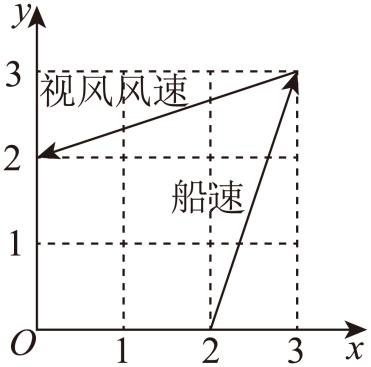
\includegraphics[width=.42\linewidth]{assets/asset-135-01.jpg}
\end{center}
\begin{choices}
  \item 轻风
  \item 微风
  \item 和风
  \item 劲风
\end{choices}
\begin{solution}
\textbf{答案：}A

\textbf{分析：}结合题目条件和图 2 写出视风风速对应的向量和船行风速对应的向量，求出真风风速对应的向量，得出真风风速的大小，即可由图 1 得出结论.

\textbf{详解：}由题意及图得，视风风速对应的向量为 $\vec{n} = (0,2) - (3,3) = (-3,-1)$，船行风速对应的向量为 $\overrightarrow{n_2} = -[(3,3)-(2,0)] = (-1,-3)$，设真风风速对应的向量为 $\overrightarrow{n_1}$，则 $\vec{n} = \overrightarrow{n_1} + \overrightarrow{n_2}$，所以 $\overrightarrow{n_1} = \vec{n} - \overrightarrow{n_2} = (-3,-1)-(-1,-3)=(-2,2)$，$|\overrightarrow{n_1}| = \sqrt{(-2)^2+2^2} = 2\sqrt{2} \approx 2.828$，所以由表得，真风风速为轻风，故选：A.
\end{solution}
\end{question}

\begin{question}[points=5]
\textbf{来源：}2025 年 上海卷，第 12 题\par
已知 $f(x) = \begin{cases} 1, & x > 0 \\ 0, & x = 0 \\ -1, & x < 0 \end{cases}$，$\vec{a}, \vec{b}, \vec{c}$ 是平面内三个不同的单位向量．若 $f(\vec{a} \cdot \vec{b}) + f(\vec{b} \cdot \vec{c}) + f(\vec{c} \cdot \vec{a}) = 0$，则 $|\vec{a} + \vec{b} + \vec{c}|$ 的取值范围是．
\fillin[{$(1, \sqrt{5})$}]
\begin{solution}
\textbf{答案：}$(1, \sqrt{5})$

\textbf{分析：}利用分段函数值分类讨论，可得 $\{f(\vec{a} \cdot \vec{b}), f(\vec{b} \cdot \vec{c}), f(\vec{c} \cdot \vec{a})\} = \{-1, 0, 1\}$，再根据数量积关系设出 $\vec{a}, \vec{b}, \vec{c}$ 坐标，利用坐标运算，结合三角恒等变换求解模的范围可得.

\textbf{详解：}若 $f(\vec{a} \cdot \vec{b}) = f(\vec{b} \cdot \vec{c}) = f(\vec{c} \cdot \vec{a}) = 0$，则 $\vec{a} \cdot \vec{b} = \vec{b} \cdot \vec{c} = \vec{c} \cdot \vec{a} = 0$，又三个向量均为平面内的单位向量，故向量 $\vec{a}, \vec{b}, \vec{c}$ 两两垂直，显然不成立；故 $\{f(\vec{a} \cdot \vec{b}), f(\vec{b} \cdot \vec{c}), f(\vec{c} \cdot \vec{a})\} = \{-1, 0, 1\}$ . 不妨设 $\begin{cases} f(\vec{a} \cdot \vec{b}) = 1 \\ f(\vec{b} \cdot \vec{c}) = 0 \\ f(\vec{c} \cdot \vec{a}) = -1 \end{cases}$，则 $\vec{a} \cdot \vec{b} > 0, \vec{b} \cdot \vec{c} = 0, \vec{c} \cdot \vec{a} < 0$，不妨设 $\vec{b} = (1,0), \vec{c} = (0,1)$，$\vec{a} = (\cos \theta, \sin \theta), \theta \in [0, 2\pi)$，则 $\begin{cases} \vec{a} \cdot \vec{b} = \cos \theta > 0 \\ \vec{c} \cdot \vec{a} = \sin \theta < 0 \end{cases}$，则 $\theta \in \left(\frac{3\pi}{2}, 2\pi\right)$，则 $|\vec{a} + \vec{b} + \vec{c}| = \sqrt{(1+\cos \theta)^2 + (1+\sin \theta)^2} = \sqrt{3 + 2\cos \theta + 2\sin \theta} = \sqrt{3 + 2\sqrt{2}\sin\left(\theta + \frac{\pi}{4}\right)}$，由 $\theta \in \left(\frac{3\pi}{2}, 2\pi\right)$，$\theta + \frac{\pi}{4} \in \left(\frac{7\pi}{4}, \frac{9\pi}{4}\right)$，则 $\sin\left(\theta + \frac{\pi}{4}\right) \in \left(-\frac{\sqrt{2}}{2}, \frac{\sqrt{2}}{2}\right)$，$2\sqrt{2}\sin\left(\theta + \frac{\pi}{4}\right) \in (-2, 2)$，故 $|\vec{a} + \vec{b} + \vec{c}| \in (1, \sqrt{5})$ .
\end{solution}
\end{question}

\begin{question}[points=5]
\textbf{来源：}2025 年 天津卷，第 14 题\par
$\triangle ABC$中, $D$为$AB$边中点, $\overrightarrow{CE} = \dfrac{1}{3}\overrightarrow{CD}$, $\overrightarrow{AB} = \vec{a}$, $\overrightarrow{AC} = \vec{b}$, 则$\overrightarrow{AE} = $（用$\vec{a}$, $\vec{b}$表示）, 若$|\overrightarrow{AE}| = 5$, $\overrightarrow{AE} \perp \overrightarrow{CB}$, 则$\overrightarrow{AE} \cdot \overrightarrow{CD} = $.
\fillin[{$\dfrac{1}{6}\vec{a} + \dfrac{2}{3}\vec{b}$；$-15$}]
\begin{solution}
\textbf{答案：}$\dfrac{1}{6}\vec{a} + \dfrac{2}{3}\vec{b}$；$-15$

\textbf{分析：}根据向量的线性运算求解即可空一，应用数量积运算律计算求解空二.

\textbf{详解：}如图，因为$\overrightarrow{CE} = \dfrac{1}{3}\overrightarrow{CD}$, 所以$\overrightarrow{AE} - \overrightarrow{AC} = \dfrac{1}{3}(\overrightarrow{AD} - \overrightarrow{AC})$, 所以$\overrightarrow{AE} = \dfrac{1}{3}\overrightarrow{AD} + \dfrac{2}{3}\overrightarrow{AC}$. 因为$D$为线段$AB$的中点, 所以$\overrightarrow{AE} = \dfrac{1}{6}\overrightarrow{AB} + \dfrac{2}{3}\overrightarrow{AC} = \dfrac{1}{6}\vec{a} + \dfrac{2}{3}\vec{b}$. 又因为$|\overrightarrow{AE}| = 5$, $\overrightarrow{AE} \perp \overrightarrow{CB}$, 所以$|\overrightarrow{AE}|^2 = \left(\dfrac{1}{6}\vec{a} + \dfrac{2}{3}\vec{b}\right)^2 = \dfrac{1}{36}|\vec{a}|^2 + \dfrac{2}{9}\vec{a}\cdot\vec{b} + \dfrac{4}{9}|\vec{b}|^2 = 25$, $\overrightarrow{AE} \cdot \overrightarrow{CB} = \left(\dfrac{1}{6}\vec{a} + \dfrac{2}{3}\vec{b}\right)\cdot(\vec{a} - \vec{b}) = \dfrac{1}{6}|\vec{a}|^2 + \dfrac{1}{2}\vec{a}\cdot\vec{b} - \dfrac{2}{3}|\vec{b}|^2 = 0$, 所以$|\vec{a}|^2 + 3\vec{a}\cdot\vec{b} = 4|\vec{b}|^2$. 所以$|\vec{a}|^2 + 4\vec{a}\cdot\vec{b} = 180$, 所以$\overrightarrow{AE} \cdot \overrightarrow{CD} = \left(\dfrac{1}{6}\vec{a} + \dfrac{2}{3}\vec{b}\right)\cdot\left(-\vec{b} + \dfrac{1}{2}\vec{a}\right) = \dfrac{1}{12}|\vec{a}|^2 + \dfrac{1}{6}\vec{a}\cdot\vec{b} - \dfrac{2}{3}|\vec{b}|^2 = \dfrac{1}{12}(|\vec{a}|^2 + 2\vec{a}\cdot\vec{b} - 8|\vec{b}|^2) = \dfrac{1}{12}(|\vec{a}|^2 + 2\vec{a}\cdot\vec{b} - 2(|\vec{a}|^2 + 3\vec{a}\cdot\vec{b})) = \dfrac{1}{12}(-|\vec{a}|^2 - 4\vec{a}\cdot\vec{b}) = -\dfrac{1}{12}(|\vec{a}|^2 + 4\vec{a}\cdot\vec{b}) = -\dfrac{180}{12} = -15$. 故答案为$\dfrac{1}{6}\vec{a} + \dfrac{2}{3}\vec{b}$；$-15$.
\end{solution}
\end{question}

\begin{question}[points=15]
\textbf{来源：}2025 年 天津卷，第 16 题\par
在$\triangle ABC$中, 角$A, B, C$的对边分别为$a, b, c$. 已知$a\sin B = \sqrt{3}b\cos A$, $c - 2b = 1$, $a = \sqrt{7}$.

(1) 求$A$的值;

(2) 求$c$的值;

(3) 求$\sin(A + 2B)$的值.
\begin{solution}

\textbf{分析：}(1)由正弦定理化边为角再化简可求；(2)由余弦定理，结合(1)结论与已知代入可得关于$b$的方程，求解可得$b$，进而求得$c$；(3)利用正弦定理先求$B$，再由二倍角公式分别求$\sin 2B$, $\cos 2B$，由两角和的正弦可得.

\textbf{详解：}（1）已知$a\sin B = \sqrt{3}b\cos A$, 由正弦定理$\dfrac{a}{\sin A} = \dfrac{b}{\sin B}$, 得$a\sin B = b\sin A = \sqrt{3}b\cos A$, 显然$\cos A \neq 0$, 得$\tan A = \sqrt{3}$, 由$0 < A < \pi$, 故$A = \dfrac{\pi}{3}$.
（2）由（1）知$\cos A = \dfrac{1}{2}$, 且$c = 2b + 1$, $a = \sqrt{7}$, 由余弦定理$a^2 = b^2 + c^2 - 2bc\cos A$, 则$7 = b^2 + (2b+1)^2 - 2 \times \dfrac{1}{2} b(2b+1) = 3b^2 + 3b + 1$, 解得$b = 1$（$b = -2$舍去）, 故$c = 3$.
（3）由正弦定理$\dfrac{a}{\sin A} = \dfrac{b}{\sin B}$, 且$b = 1$, $a = \sqrt{7}$, $\sin A = \dfrac{\sqrt{3}}{2}$, 得$\sin B = \dfrac{b\sin A}{a} = \dfrac{\sqrt{21}}{14}$, 且$a > b$, 则$B$为锐角, 故$\cos B = \dfrac{5\sqrt{7}}{14}$, 故$\sin 2B = 2\sin B\cos B = \dfrac{5\sqrt{3}}{14}$, 且$\cos 2B = 1 - 2\sin^2 B = 1 - 2 \times \left(\dfrac{\sqrt{21}}{14}\right)^2 = \dfrac{11}{14}$; 故$\sin(A + 2B) = \sin A \cos 2B + \cos A \sin 2B = \dfrac{\sqrt{3}}{2} \times \dfrac{11}{14} + \dfrac{1}{2} \times \dfrac{5\sqrt{3}}{14} = \dfrac{4\sqrt{3}}{7}$.
\end{solution}
\end{question}

